\documentclass[10pt,letterpaper]{article}

%% -packages-
\usepackage{graphicx}
\usepackage{epstopdf}
\usepackage{psfrag}
\usepackage[round]{natbib}
\usepackage{longtable}
\usepackage{rotating}
\usepackage{rotate}
\usepackage{lscape}
\usepackage{amssymb}
\usepackage{amsmath}
\usepackage[colorlinks,bookmarks,citecolor=magenta]{hyperref}
\usepackage{color}
\usepackage{multicol}
\usepackage{alltt}
\usepackage{listings}


\lstset{ %
language=R,                % choose the language of the code
basicstyle=\footnotesize,       % the size of the fonts that are used for the code
numbers=left,                   % where to put the line-numbers
numberstyle=\footnotesize,      % the size of the fonts that are used for the line-numbers
stepnumber=2,                   % the step between two line-numbers. If it's 1 each line 
                                % will be numbered
numbersep=5pt,                  % how far the line-numbers are from the code
backgroundcolor=\color{white},  % choose the background color. You must add \usepackage{color}
showspaces=false,               % show spaces adding particular underscores
showstringspaces=false,         % underline spaces within strings
showtabs=false,                 % show tabs within strings adding particular underscores
frame=single,                   % adds a frame around the code
tabsize=2,                      % sets default tabsize to 2 spaces
captionpos=b,                   % sets the caption-position to bottom
breaklines=true,                % sets automatic line breaking
breakatwhitespace=false,        % sets if automatic breaks should only happen at whitespace
title=\lstname,                 % show the filename of files included with \lstinputlisting;
                                % also try caption instead of title
escapeinside={\%*}{*)},         % if you want to add a comment within your code
morekeywords={*,...}            % if you want to add more keywords to the set
}



%\usepackage[latin1]{inputenc} % To use characters such as � without typing \'e
%\usepackage[cyr]{aeguill} % To display characters such as �
%\usepackage{xspace} % To get the right spacings in front of : and so on
\usepackage[french,english]{babel}

%% ---------------------------------------------------------------------
%%Page Layout Properties-------------------------------------------------

%\voffset 0in \textwidth 7.0in  \oddsidemargin 0in
%\evensidemargin 0in \headheight 0.in \textheight 9in  %%Look at Box13.1 for text scale
\voffset -0.75in
\hoffset -0.75in
\textwidth 6.5in%
\textheight 8.5in%
%\evensidemargin 0.in%

%\textwidth 6in%
%\topmargin 0in%
\setlength{\LTcapwidth}{\textwidth} %caption width for longtables

%Arial font
\renewcommand{\rmdefault}{ppl} % Arial
\renewcommand{\sfdefault}{ppl} % Arial phv  % palatino ppl

	
	
%Logo
\usepackage{fancyhdr}
\renewcommand{\headheight}{0.6in}
\setlength{\headwidth}{\textwidth}
\fancyhead[L]{}% empty left
\fancyhead[R]{ % right
   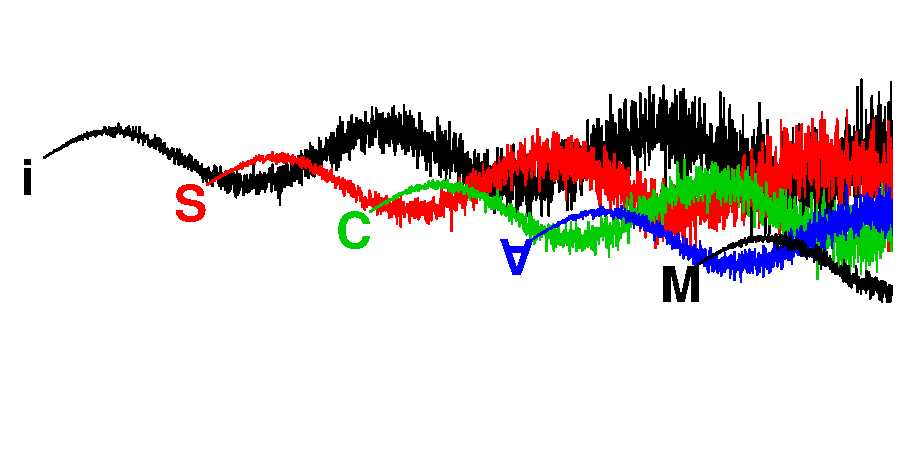
\includegraphics[height=0.53in]{iscamlogo.eps}
}
\pagestyle{fancy}

% %Logo
% \usepackage{fancyhdr}
% \renewcommand{\headheight}{0.6in}
% \setlength{\headwidth}{\textwidth}
% \fancyhead[L]{}% empty left
% \fancyhead[R]{ % right
%    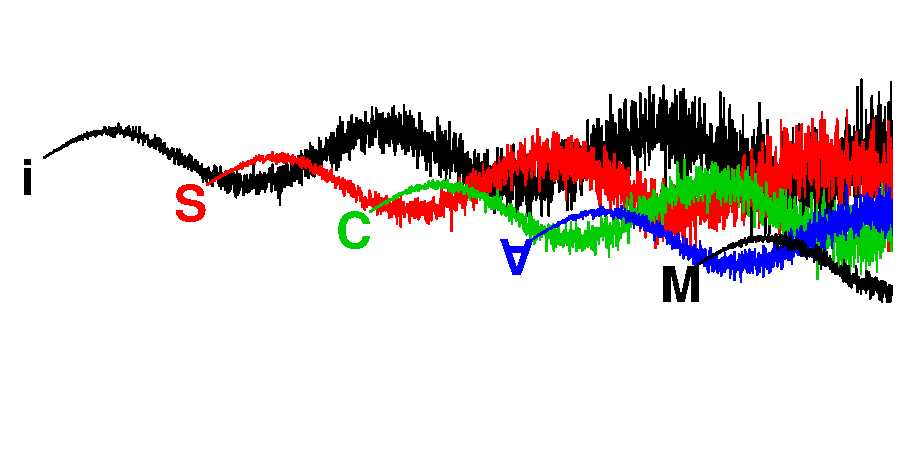
\includegraphics[height=0.53in]{iscamlogo.eps}
% }
% \pagestyle{fancy}


%-------------------------------------------------------------------------
%Water mark
%%\usepackage{eso-pic}
%%\usepackage{graphicx}
%%\usepackage{color}
%%\usepackage{type1cm}
%%\usepackage{float} 
%%
%%\makeatletter
%%  \AddToShipoutPicture{%
%%    \setlength{\@tempdimb}{.5\paperwidth}%
%%    \setlength{\@tempdimc}{.5\paperheight}%
%%    \setlength{\unitlength}{1pt}%
%%    \put(\strip@pt\@tempdimb,\strip@pt\@tempdimc){%
%%      \makebox(0,0){\rotatebox{45}{\textcolor[gray]{0.85}{\fontsize{1.75cm}{1.75cm}\selectfont{DRAFT  \today}}}}
%%    }
%%} \makeatother


%% -math-
\newcounter{saveEq}
  \def\putEq{\setcounter{saveEq}{\value{equation}}}
  \def\getEq{\setcounter{equation}{\value{saveEq}}}
  \def\tableEq{ % equations in tables
    \putEq \setcounter{equation}{0}
    \renewcommand{\theequation}{T\arabic{table}.\arabic{equation}}
    \vspace{-5mm}
    }
  \def\normalEq{ % renew normal equations
    \getEq
    \renewcommand{\theequation}{\arabic{section}.\arabic{equation}}}

  \def\puthrule{ %thick rule lines for equation tables
    \hrule \hrule \hrule \hrule \hrule}


%%\newcommand{\msy}{$C^*$}
%%\newcommand{\fmsy}{$F^*$}
%%\newcommand{\sbmsy}{$\rm{SB_{MSY}}$}
%%\newcommand{\sbfour}{$\rm{SB_{40}}$}
%%\newcommand{\�}{\'e}
%%\newcommand{\�}{\`e}
%%\newcommand{\�}{\`a}
%%\newcommand{\�}{\^e}
%\newcommand{\iscam}{
%{$^i$}\textcolor{red}{S}\textcolor{green}{\small{}C}{\textcolor{blue}{\footnotesize{}A%}}\textcolor{black}{$_\textnormal{M}$}}%{\raisebox{-0.7ex}{M}}%

%\input logo.sty


\newcommand{\fmsy}{F$_{\textnormal{MSY}}$}
\newcommand{\bmsy}{B$_{\textnormal{MSY}}$}

%% ---------------------------------------------------------------------


\makeatletter
\newenvironment{tablehere}
  {\def\@captype{table}}
  {}

\newenvironment{figurehere}
  {\def\@captype{figure}}
  {}
\makeatother

%iscam logo
\newcommand{\iscam}{
	\raisebox{0.75ex}{$i$}%
	\textcolor{red}{\raisebox{0.25ex}{S}}%
	\textcolor{green}{\raisebox{0.00ex}{C}}%
	\textcolor{blue}{\raisebox{-.25ex}{A}}%
	\raisebox{-.50ex}{M}%
	}%


%% ---------------------------------------------------------------------


\title{
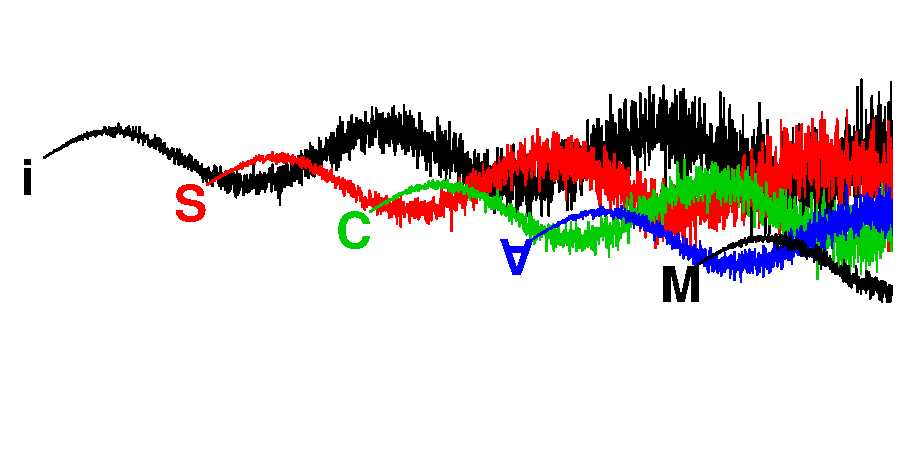
\includegraphics[height=2.53in]{iscamlogo.eps}
\vfill
\iscam\ Users Guide\\
Version 1.0\\
\vfill}
\author{Steven Martell\\
University of British Columbia\\
Fisheries Centre\\
2202 Main Mall\\
Vancouver, BC\\
V6T 1Z4\\
Canada\\ 
\texttt{s.martell@fisheries.ubc.ca}}
\date{\small{$^\copyright$  Copyright Steven Martell, \today.  All rights reserved.}}







\begin{document}

\pagenumbering{roman}
\setcounter{page}{1}
    \maketitle \thispagestyle{empty}
%    \vfill
%    \noindent\hrulefill\\
%    Draft document for peer review: Started on Wednesday, February 11, 2009\\
%    Draft document completed on Thursday, February 19, 2009\\
%    Final document completed on Wednesday, March 4, 2009.\\
%    CSAS revisions completed on Wednesday, March 11, 2009.
%    \clearpage
\thispagestyle{empty}
\clearpage


\newpage


%\begin{abstract}
%This is the abstract
%  \end{abstract}
%\clearpage


%%
 \selectlanguage{english}

    %\input{ToDoList}
%% -Executive summary material------------------------------------------

\pagenumbering{roman}
\section*{Preface}
\addcontentsline{toc}{subsection}{Preface}
This document is the users guide for the fisheries stock assessment model \iscam, or Integrated Statistical Catch Age model.  This assessment package was written by Steven Martell and may be freely used by others, but in no way am I responsible for the mess that may or may not happen if you use this software to do your job.  Although I try hard, I cannot guarantee that this application is 100\% free of bugs/coding errors so double check your own work and see if it makes sense.  If you find a bug, fix it, recompile the code and continue on.  Or let me know about the bug and I'll happily  fix it for you,  if I have time.


\section*{Acknowledgements}
\addcontentsline{toc}{subsection}{Preface}
I greatly appreciate the early feedback I received from Jake Schweigert (DFO Pacific Biological Satiation, Nanaimo, BC) while developing this software and the users guide.  Also feedback, error checking, and code from Vivian Haist, Jim Ianelli, Robyn Forrest and Chris Grandin.  Much of the linkage between ADMB and R was inspired by my DFO colleagues and friends, Rob Kronlund, Jon Schnute, and Jaclyn Cleary.


%%%!TEX root = /Users/stevenmartell/Documents/CURRENT PROJECTS/iSCAM-trunk/fba/BC-herring-2011/WRITEUP/BCHerring2011.tex


%\subsection*{Abstract}
%\addcontentsline{toc}{subsection}{Abstract}
%
%June 15, 2011.  Structure of this paper has changed a bit. This document will now consist of an assessment and forecast of the five major stocks and the two minor stocks.  There will be at least 5 appendixes that 1) describe the input data and the control files used for the assessment model, 2) a detailed description of \iscam, 3) a description of the methods used to develop the prior distribution, 4) simulation testing of the \iscam model, 5) moving toward the sustainable fisheries framework (see Cleary and Cox paper) and include discussion of the issues of developing an MSY-based framework for a multigear fishery with changing selectivities and natural mortality rates, and finally 6) a list of research recommendations.
%
%Summary:  Three major themes of the paper: 1) a comparing HCAM and iSCAM (where iSCAM is set up with nearly the same assumptions as 2010 HCAM assessment), 2) an iSCAM assessment with several scenarios addressing (a) q with various priors, (b) time-varying versus constant M, (c) alternative selectivity models, and (d) the interactions of all three of these confounded variables, and 3) an iSCAM assessment with the test fishery and seine roe fishery data separated into specific fleets.  The side by side comparison will examine similarities/differences between trends in biomass, fishing mortality rates, and residual fits to the spawn survey data an age-composition data.  These two models have some fundamental differences in the statistical assumptions about the catch-at-age data, so results are likely to be slightly different.  Results for all three themes will focus on reconstructing table 5 from last years assessment, with the addition of LRP and USRP to be compared with the cuttoffs and catch advice for low med and high recruitment.
%


\section*{Abstract}\addcontentsline{toc}{section}{Abstract}

Estimates of herring abundance in British Columbia (B.C.) waters  has been based on catch-age data and spawn survey abundance information.  These data are typically interpolated using a statistical catch-age framework; however, virtual methods (e.g., VPA) have been used in the past. This assessment also uses a statistical catch age model.  This document is broken into two parts: Part I deals with moving the herring assessments towards Canada's sustainable fisheries framework and introduces a new integrated statistical catch-age model for jointly estimating the abundance of Pacific herring and associated reference points to be used in the sustainable fisheries framework.  Part II of this document  implements this new assessment framework using the data for the five major and two minor regions.  Finally, we present catch advice based on decision tables that utilize poor, average, and good age-3 recruitment forecasts.

In Part I of this document we provide a very brief description of the new assessment framework (a full technical description of the model is provided in the Appendix of this document).  We then conduct some simulation testing with perfect information to  demonstrate that the model is capable of estimating all the parameters. We further explore precision and bias in parameter estimates based on simulation data with both observation and process errors.  We then parameterize the new assessment model such that the assumptions of the previous assessment model (Herring Catch Age Model, or HCAM) are mostly met and compare parameter estimates and estimates of spawning stock biomass (using data from 1951:2010).  Using data from the Strait of Georgia only, we then compare alternative assumptions about the spawn survey scaling coefficient ($q$), natural mortality and selectivity, and examine how these alternative assumptions influence estimates of key parameters (unfished spawning biomass, steepness, average natural mortality).  Relaxing assumptions about $q$ and natural mortality rates had the largest impacts on estimated parameters.  Lastly, we compared estimates of spawning stock biomass from HCAM with the new model for all five major areas to understand the subtle differences between the assumptions in the two models.% \footnote{At the time of writing this document and submitting it for peer review, an error was notices in the formulation of the weight-based selectivity function for the gill net fishery.  This error has been corrected for all of the results presented in Part II, but has still to be corrected for the model comparisons in Part I of this document.  Time permitting, these comparisons will be conducted prior to the assessment meeting, and if not at least presented at the September 7, 2011 meeting.}.

In Part II of this document we present updated data from the herring fisheries and surveys in 2011, a brief description of the analytical methods used to construct the decision tables, and present the results of the application of the new assessment model to the 2011 data. New this year is a Bayesian prior for the dive survey spawn index ($q$) and the development of this prior is detailed in the appendix.  The expected value of $q$ was estimated to be 0.587 with a standard deviation of 0.155. To summarize the overall fit to the model, maximum likelihood estimates derived quantities and residuals between observed and predicted variables are used.  Retrospective analysis (i.e., the sequential removal of the most recent data) is used as a diagnostic for model misspecification.   Catch advice (decision tables) are based on the median values of random samples from the joint posterior distribution and not the maximum likelihood estimates.  Visual inspection of the trace plots from the posterior samples and pair plots were used to judge if the samples were taken from a stationary distribution. Historically catch advice was based on cuttoff values that were derived from 1996 estimates of the unfished biomass (\bo, cuttoff values are set at 0.25\bo).  This assessment provides updated estimates of \bo\ and presents catch advice based on new cuttoff values.  An alternative decision table, where catch advice is based on old cuttoffs, is also presented.  

Median estimates of the 2011 spawning stock biomass is as follows: Haida Gwaii (HG) --16,579 t, Prince Rupert District (PRD) -- 27,046 t, Central Coast (CC) -- 14,666 t, Strait of Georgia (SOG) 125,261 t, West Coast Vancouver Island (WCVI) 14,679 t.  Implementation of the current harvest control rule (HCR) advises no fishing in HG under poor recruitment and no fishing in CC under poor and average recruitment.  Based on the 20\% harvest rate and application of the harvest control rule the estimated maximum available harvest ranges from 4,296 t in HG to 27,690t in SOG (assuming good recruitment).  Catch advice for the minor areas is based on a 10\% fixed exploitation rate with no cuttoffs and ranges from 91 t in Area 27 (assuming poor recruitment) to 614 t in Area 2W (assuming good recruitment).

%\section*{Executive summary}\addcontentsline{toc}{section}{Executive summary}


\newpage
\tableofcontents
\addcontentsline{toc}{subsection}{Contents}
\newpage
%% -Main body of the document-------------------------------------------
\pagenumbering{arabic}
	
%    %!TEX root = /Users/stevenmartell1/Documents/iSCAM-project/docs/iSCAM-guide/userGuide/usrGuide.tex

\section{Introduction} % (fold)
\label{sec:introduction}
\begin{multicols}{2}
	The purpose of this users guide is to aid in the development of new assessment models using \iscam\ and to document the code. \iscam{} is written in \admb{} and the source code is freely available.  This manual was written in \LaTeX{}.

\subsection{Overview of iSCAM} % (fold)
\label{sub:overview}
As an AD Model builder program, \iscam\ has several input files and several output files along with the executable program that actually performs the non-linear parameter estimation and all other model calculations.  There are three input files required:
\begin{enumerate}
	\item iscam.dat
	\item $<$data file$>$
	\item $<$control file$>$
\end{enumerate}
 All three files are required to run \iscam, and the files are read in the order presented above.  The iscam.dat file contains only the file names of the data file and the control file.  The data file contains all of the necessary data for a particular stock including, model dimensions, life-history information, time series data on observed catch, the relative abundance indices and information on age-compositions sampled from each of the fisheries.
 
 The control file contains the necessary information for setting bounds and priors for estimated model parameters, specifying the types of selectivity curves for each of the fisheries, and other miscellaneous controls for producing various outputs and weighing components of the objective function.  Note that \iscam\ is intended to have a lot of flexibility, but with this flexibility comes at a cost of being more difficult to rapidly develop models and obtain reasonable parameter estimates.
 
 \iscam\ also has a custom command line option for conducting simulation trials based on the observed data set. In a simulation trial, the historical data and known parameter values are used to simulate observed data with known assumptions. Following the simulation, the model then estimates the model parameters.   This is an important feature to ensure that your model set up is capable of estimating the true parameter values, or used in simulation-estimation experiments for exploring estimability and parameter bias.
 
 There are a number of standard report files produced by AD Model Builder programs, and in addition to these report files, there are additional custom files for dealing with the MCMC output from \iscam.

% subsection overview_of_is (end)

\subsection{Obtaining \iscam{}} % (fold)
\label{sub:obtaining_iscam}
\iscam\ can be freely obtained from a google code repository \url{http://code.google.com/p/iscam-project/}.  %Or by directly emailing \href{mailto:s.martell@fisheries.ubc.ca}{Steven Martell}.



% subsection obtaining_iscam (end)

\end{multicols}
% section introduction (end)










% \setlength{\columnseprule}{1pt}
% \setlength{\columnsep}{20pt}
% 
% \begin{multicols}{2}
% \section{Introduction}
%  The purpose of this users guide is to aid in the development of new assessment models using \iscam\ and to document the code. \iscam\ is written in AD Model Builder and the source code is freely available.
% 
% %\subsection{Overview}
% As an AD Model builder program, \iscam has several input files and several output files along with the executable program that actually performs the non-linear parameter estimation and all other model calculations.  There are three input files required:
% \begin{enumerate}
% 	\item iscam.dat
% 	\item $<$data file$>$
% 	\item $<$control file$>$
% \end{enumerate}
%  All three files are required to run \iscam\, and the files are read in the order presented above.  The iscam.dat file contains only the file names of the data file and the control file.  The data file contains all of the necessary data for a particular stock including, model dimensions, life-history information, time series data on observed catch, the relative abundance indices and information on age-compositions sampled from each of the fisheries.
%  
%  The control file contains the necessary information for setting bounds and priors for estimated model parameters, specifying the types of selectivity curves for each of the fisheries, and other miscellaneous controls for producing various outputs and weighing components of the objective function.  Note that \iscam\ is intended to have a lot of flexibility, but with this flexibility comes at a cost of being more difficult to rapidly develop models and obtain reasonable parameter estimates.
%  
%  \iscam\ also has a custom command line option for conducting simulation trials based on the observed data set. In a simulation trial, the historical data and known parameter values are used to simulate observed data with known assumptions. Following the simulation, the model then estimates the model parameters.   This is an important feature to ensure that your model set up is capable of estimating the true parameter values, or used in simulation-estimation experiments for exploring estimability and parameter bias.
%  
%  There are a number of standard report files produced by AD Model Builder programs, and in addition to these report files, there are additional custom files for dealing with the MCMC output from \iscam. 
%  
%  \subsection{Obtaining \iscam\}
%  \iscam can be freely obtained from (website).  Or by directly emailing \href{mailto:s.martell@fisheries.ubc.ca}{Steven Martell}.
%  
% \end{multicols}

    %!TEX root = /Users/stevenmartell1/Documents/iSCAM-project/docs/iSCAM-guide/userGuide/usrGuide.tex


\section{Running \iscam: input files \& command line options} % (fold)
\label{sec:running_iscam_input_files_&_command_line_options}

\begin{multicols}{2}


There are four required input files for \iscam: the \verb"iscam.dat" file, the \verb"datafile",  the \verb"controlfile", and the \verb"projectionfile".  By default when \iscam runs, the first file it looks for is the \verb"iscam.dat" file, unless otherwise specified by using the command line option \verb"-ind".  The following subsections explains the details of each of the data files.


%%%%%%%%%%%%%%%%%%%%%%%%%%%%%%%%%%%%%%%%%%%
\subsection{The \texttt{iscam.dat} file}
What is required in the \verb"iscam.dat" file is just the name of the data file and the control file, in that order.  An example is given below for the \texttt{PHake2010.dat} and \texttt{Phake2010.ctl} data and control files.
\begin{verbatim}
PHake2010.dat       #Data file name
PHake2010.ctl       #Control file name
PHake2010.pfc       #Projection file name
\end{verbatim}
Note that it is necessary to have the \verb"*.dat", and \verb"*.ctl" extensions, as \iscam\ will read in the entire filename including the extension.  Also note that the \verb"#" symbol acts as a comment line, and \iscam\ will ignore the contents of the remaining line when reading in data. Lastly, the order of the files is always data file, control file, and projection file.

%%%%%%%%%%%%%%%%%%%%%%%%%%%%%%%%%%%%%%%%%%%
\subsection{The Data File} % (fold)
\label{sub:the_data_file}




\emph{The data file and how it is set up is very important in ensuring that \iscam\ works correctly.}  In this section I have broken down the description of the data file into several blocks that deal with model dimensions, age-schedule information, removal data from each commercial and sampling gears, relative abundance information that may come from one or all of the gears,  a description of the age composition, and finally empirical weight-at-age data.  There are some data elements that are \emph{mandatory} (e.g., dimensions, age-schedule information, removals for each gear) and some optional data.  For example it is not necessary to have relative abundance information for each of the gear-type each year, or even any information on relative abundance.  Nor is it necessary to have age-composition each and every year for every gear type; in fact, it's not necessary to have any age-composition data, but in such cases selectivity parameters will have to be fixed.


The data file is composed of several required sections (required in the sense that they must be defined, but do not necessarily have to have data).  The first of these required sections is the model dimensions.  Below is an example where the model starts in 1977 and the last year is 2009, the youngest age-group is 1 years old, and the oldest age-group is 15 years old and older (i.e., a plus group).  The total number of unique gears, including survey gears or gears that harvest roe products such as a spawn on kelp fishery.  For each of the gears an allocation of the total annual TAC for commercial fisheries must be specified in order to properly determine the MSY-based reference points for 2 or more fleets.  Again the \verb"#" is a comment character and \iscam\ will ignore the contents after this character.  The following is an example of the model dimensions section with 3 gear types, and the allocation is given 40\% to gear 1, 60\% to gear 2, and 0\% for gear three (in this case a biological survey):
\end{multicols}
\begin{verbatim}
    ## ------------------------------------------------------------------------- ##
    ## MODEL DIMENSIONS                                                          ##
    ## ------------------------------------------------------------------------- ##
    1968        # -first year of data           (syr)
    1979        # -last year of data            (nyr)
    3           # -age of youngest age class    (sage)
    9           # -age of plus group            (nage)
    3           # -number of gears              (ngear)
    ##
    ## ------------------------------------------------------------------------- ##
    ## Allocation for each gear in (ngear), use 0 for survey gears.              ##
    ## ------------------------------------------------------------------------- ##
    0.4   0.6   0.0
    ##
\end{verbatim}
\begin{multicols}{2}
The next required section is the age-schedule information pertaining to natural mortality, growth and maturity-at-age. For now, natural mortality is assumed to be age-independent.
\begin{verbatim}
## ________________________
## ___Age-schedules info___
#natural mortality rate (m)
0.23
#growth parameters (linf,k,to)
52, 0.32, 0
#length-weight allometry (a,b)
5e-6, 3.0
#maturity at age (am=log(3)/k) 
#& gm=std for logistic
3.45, 0.35
## ________________________
\end{verbatim}

Next is the time series data for the historical catch by year, fishery(ies) and survey(s).  Note that it is assumed that catch exists for each year that is specified in the model dimensions section (e.g., 1977-2009).  The first column is the year of the catch, and the subsequent columns are catch (in weight) for each fishery or survey.  Years where there are no catches (or no fishery) should be replaced by a 0.  In cases where surveys did not exist, or there were no removals (e.g., an acoustic survey), specify a zero catch for each year (row).  
\begin{verbatim}
## ________________________
#Time series data
#Observed catch 
#(1977-2009, 1,000,000 metric t)
#yr	commercial survey
1977 0.132693 0
1978 0.103639 0
1979 0.137115 0
...  omitted data for space
2008 0.321546 0
2009 0.176671 0
## ________________________
\end{verbatim}

The next section pertains to the relative abundance index, where first the number (\texttt{nit}) specified the number of independent surveys, and the next row specifies the number of observations (\texttt{nit\_nobs} ,or rows of data for each survey).  The first column is an integer vector that is used to index the survey year, the second column is the actual survey abundance index, and the third column is the gear index associated with this gear.  The fourth column is the relative weight that should be used for the index.  For example, setting wt=0 for a given year will result in omitting the data, or setting wt=2 would imply that the CV is one half of the other values.  The last column specifies the fraction of total mortality that has occurred when the survey was conducted (e.g., if the survey is conducted half way through the year then 0.5 implies that 1/2 of $Z_{t,a}$ has occurred when the survey was conducted).
\begin{verbatim}
## ________________________
#Relative Abundance index from 
#independent survey (it) 1970-2008
#nit
1
#nit_nobs
13
#iyr    it gear wt survey timing
1977 1.915  2  1   0.5
1980 2.115  2  1   0.5
1983 1.647  2  1   0.5
1986 2.857  2  1   0.5
...omitted data for space
2007 0.879  2  2   0.5
2009 1.460  2  0   0.5
## ________________________
\end{verbatim}

For age-composition information, a 3 dimensional ragged array is used to store the information by gear-type (matrix), by year (rows of each matrix) and by age (columns of each matrix).  An example of the age composition data is shown in Table \ref{T1} on page \pageref{T1}.  

First you must specify the number of gears for which age-composition data exists.  If there are no data, then set this to 0. On  the next line you must specify the number of years of age-composition data there are for each gear type.  Next, for each gear type for which age-composition data is available, you must specify the first age-class of the data, and on the next row specify the oldest age-class of the data.  In the example on page \pageref{T1}, there are two gears, the first gear has 33 years of observations, and the second gear has 13 years of observations.  Each gear has the youngest age-class at 2 years and the oldest age-class at 15 years.  This means there are 14 columns of age-compositions for each gear type. 

\iscam\ treats the age-composition data as a ragged object to avoid having to read in years of missing age-composition data.  The year and gear indexes in the first two columns are used to extract predicted age-proportions to be used in the statistical comparison (negative loglikelihoods).

The first two columns of the age-composition data refer to the year and gear type from which the data were obtained.  So in the example on the next page, the first 33 rows of the matrix (some of which is missing so it could fit on the page) corresponds to the years 1977-2009 for gear type 1, and from 1977 to 2009 every 2-3 years for gear type 2.  At present \iscam\ weights each row for each gear type equally, future versions of \iscam\ will probably have a third column here where relative weights based on effective samples sizes can be specified for each observed age-composition data.

\emph{Empirical weight-at-age} data can be optionally specified immediately following the age-composition data.  By default, \iscam\ first constructs the observed weight-at-age data based on the age-schedule information specified earlier in the data file.  If there is a partial or complete set of empirical weight-at-age data available, then the default weights-at-age are overwritten for the years in which empirical data are available.    First you must specify the number of years of observed weight-at-age data as this dimensions the matrix to read in the data.  Following is a matrix where the first column specifies the corresponding year the data were collected, and for each age class defined in the model dimensions (youngest age class to plus group age class), the observed mean weights at age must be specified.  Note that the units must be in kilograms so that unit consistency in the conversion from numbers-at-age to weight-at-age can be maintained.
\begin{footnotesize}
\begin{verbatim}
#n_wt_obs
5
#Empirical mean weight-at-age in kilograms 
#A$yr  V1   V2   V3   V4   V5   V6   V7   V8   V9
1951 0.04 0.08 0.11 0.13 0.15 0.17 0.20 0.18 0.18
1952 0.04 0.08 0.11 0.13 0.15 0.17 0.16 0.17 0.18
1953 0.03 0.07 0.09 0.12 0.14 0.15 0.13 0.17 0.18
1954 0.04 0.08 0.10 0.12 0.15 0.17 0.17 0.18 0.18
1955 0.04 0.08 0.10 0.12 0.14 0.17 0.17 0.17 0.18
\end{verbatim}
\end{footnotesize}


The last component of the data file is an end of file ``eof'' marker, which is set to 999.  This is the last number read in from the datafile and \iscam\ checks to ensure it is 999.  If there is an error reading the datafile, \iscam\ will break and report that there was an error reading the data.


\begin{verbatim}
## ________________________
#eof
999
## ________________________
\end{verbatim}

\end{multicols}
%\begin{minipage}[b]{\linewidth}
%\centering
\begin{landscape}
\begin{table}
\caption{Example of age composition data in the data file.}\label{T1}
\begin{scriptsize}
\begin{verbatim}
#Age composition data by year, gear (ages 2-15+)
#na_gears
2
#na_nobs
33	13
#a_sage
2	2
#a_page
15	15
#yr 	gear       V1       V2       V3       V4       V5       V6       V7       V8       V9      V10      V11      V12      V13      V14
1977    1 0.091087 0.039290 0.208628 0.028500 0.053160 0.211179 0.078270 0.079949 0.063640 0.058483 0.043761 0.029639 0.007592 0.006823
1978    1 0.022968 0.101932 0.068633 0.199094 0.033354 0.071961 0.208406 0.084622 0.072156 0.073040 0.024682 0.021006 0.013116 0.005030
1979    1 0.049457 0.089640 0.100254 0.046571 0.191908 0.071243 0.159754 0.158389 0.056370 0.037676 0.016184 0.010295 0.006469 0.005789
1980    1 0.009331 0.254593 0.042151 0.054263 0.050507 0.143816 0.065236 0.087843 0.169471 0.046122 0.037636 0.023076 0.008874 0.007079
1981    1 0.091224 0.062768 0.280898 0.012851 0.045430 0.047641 0.148751 0.062707 0.066417 0.125977 0.031183 0.012419 0.009671 0.002062
1982    1 0.181412 0.025886 0.016978 0.318964 0.032603 0.045648 0.045099 0.131034 0.027439 0.033879 0.119575 0.010972 0.006862 0.003648
1983    1 0.000322 0.327381 0.030386 0.021774 0.318861 0.034486 0.037515 0.044368 0.095257 0.024331 0.017871 0.037722 0.007340 0.002385
1984    1 0.000000 0.010415 0.546489 0.035445 0.072340 0.185115 0.023775 0.020842 0.014283 0.045333 0.009533 0.007920 0.024390 0.004121
1985    1 0.006798 0.006334 0.065169 0.607023 0.070421 0.058060 0.132423 0.011557 0.006879 0.007111 0.013539 0.002836 0.000000 0.011849
1986    1 0.111570 0.031159 0.007757 0.034088 0.485333 0.058011 0.043959 0.122124 0.022909 0.026576 0.014536 0.026627 0.004392 0.010957
1987    1 0.000000 0.264654 0.016305 0.003861 0.017893 0.540852 0.032262 0.016639 0.080708 0.003902 0.001822 0.005542 0.009811 0.005748
1988    1 0.002907 0.002881 0.325484 0.012085 0.007047 0.010794 0.464716 0.021331 0.009870 0.101698 0.001949 0.004157 0.001274 0.033806
1989    1 0.026833 0.022546 0.009612 0.452262 0.010250 0.004556 0.006132 0.394579 0.015267 0.006758 0.044542 0.000903 0.001179 0.004583
1990    1 0.048604 0.255566 0.024077 0.002273 0.251121 0.006576 0.001663 0.000990 0.323920 0.003924 0.000212 0.072414 0.000146 0.008513
1991    1 0.034754 0.176910 0.169392 0.027073 0.007271 0.316749 0.012094 0.001274 0.001349 0.206127 0.003853 0.000000 0.036791 0.006363
1992    1 0.035191 0.044184 0.126581 0.177710 0.021788 0.007533 0.344623 0.006212 0.001264 0.003920 0.198907 0.004982 0.000449 0.026655
1993    1 0.007327 0.219650 0.032109 0.141618 0.169717 0.014288 0.007544 0.287667 0.008052 0.001062 0.000425 0.104591 0.000492 0.005457
1994    1 0.000419 0.033794 0.194593 0.013819 0.121828 0.200067 0.013059 0.004773 0.307047 0.002355 0.004118 0.000280 0.096116 0.007732
1995    1 0.015172 0.001676 0.067824 0.247580 0.011946 0.076025 0.204514 0.017753 0.003065 0.259156 0.002369 0.003815 0.000000 0.089107
...	some missing data removed here to fit on page.
2005    1 0.008720 0.004799 0.070427 0.055023 0.684012 0.084118 0.021823 0.028355 0.019809 0.010432 0.008069 0.002582 0.000360 0.001470
2006    1 0.016047 0.109332 0.016100 0.086023 0.047267 0.606611 0.050565 0.017944 0.019738 0.012433 0.009263 0.004693 0.001532 0.002454
2007    1 0.135250 0.030604 0.145496 0.015585 0.070675 0.041936 0.441809 0.059055 0.018388 0.018549 0.012342 0.004254 0.004551 0.001507
2008    1 0.086419 0.307710 0.023174 0.134343 0.009449 0.035456 0.033322 0.305151 0.032058 0.010867 0.008882 0.005414 0.003330 0.004426
2009    1 0.007237 0.201241 0.298293 0.044466 0.140682 0.014182 0.025967 0.022153 0.193496 0.036166 0.005012 0.004290 0.003855 0.002961
1977    2 0.054308 0.051673 0.322415 0.029524 0.041387 0.358094 0.049372 0.036486 0.020920 0.019594 0.010201 0.003792 0.000997 0.001237
1980    2 0.004557 0.555127 0.053761 0.032569 0.026590 0.117668 0.043603 0.093838 0.037630 0.022180 0.003734 0.006424 0.001338 0.000983
1983    2 0.000265 0.785009 0.026011 0.007869 0.103384 0.016545 0.011402 0.008131 0.022356 0.005273 0.006223 0.006489 0.001042 0.000000
1986    2 0.604601 0.015879 0.002792 0.019748 0.266035 0.028628 0.022778 0.029920 0.003627 0.003812 0.000276 0.001440 0.000463 0.000000
1989    2 0.169990 0.058515 0.012874 0.526835 0.011735 0.004161 0.007554 0.179632 0.009473 0.000722 0.017782 0.000000 0.000000 0.000726
1992    2 0.089253 0.011915 0.069071 0.176823 0.021856 0.008862 0.432238 0.013086 0.007872 0.003964 0.149487 0.007606 0.000000 0.007967
1995    2 0.324964 0.043475 0.012039 0.212541 0.009810 0.032765 0.148871 0.002177 0.000000 0.158452 0.000354 0.006429 0.000000 0.048122
1998    2 0.168351 0.187074 0.157169 0.195749 0.014026 0.055093 0.087607 0.010731 0.015903 0.048868 0.003121 0.001999 0.042448 0.011861
2001    2 0.709921 0.089531 0.052761 0.056572 0.026180 0.026069 0.014190 0.008255 0.005804 0.002446 0.002162 0.004212 0.000400 0.001496
2003    2 0.029781 0.025334 0.640666 0.109500 0.027623 0.060058 0.039723 0.021949 0.022287 0.007181 0.004232 0.004367 0.003083 0.004214
2005    2 0.239916 0.024324 0.072095 0.051813 0.482518 0.052666 0.017966 0.024352 0.013884 0.011229 0.004744 0.002436 0.000323 0.001734
2007    2 0.428146 0.024375 0.101876 0.011527 0.041221 0.026044 0.289941 0.030229 0.013473 0.013191 0.007185 0.006086 0.002778 0.003928
2009    2 0.001881 0.229516 0.423131 0.024861 0.091878 0.007856 0.018074 0.024434 0.128613 0.029027 0.009417 0.005566 0.005402 0.000343
\end{verbatim}
\end{scriptsize}
\end{table}
\end{landscape}


% subsection the_data_file (end)

%%%%%%%%%%%%%%%%%%%%%%%%%%%%%%%%%%%%%%%%%%%
\begin{multicols}{2}
\subsection{The Control File} % (fold)
\label{sub:the_control_file}


The first section of the control file pertains to the leading parameter vector which is summarized in Table \ref{Table.parameter.controls}.  For now, there are 6 leading parameters for which the initial values (ival) lower (lb) and upper bounds (ub) and estimation phase must be specified.  Each of these parameters also have parameters for the corresponding prior distributions defined by the prior\_type, and parameters p1 and p2.

\begin{tablehere}\caption{Controls for estimated parameters in the control file.}\label{Table.parameter.controls}
\begin{tiny}
\begin{verbatim}
## ____________________________________________________________________________ ##
##                            PACIFIC HAKE CONTROLS
## ___________________CONTROLS FOR ESTIMATED PARAMETERS________________________ ##
##  Prior descriptions:
##                      -0 uniform (0,0)
##                      -1 normal (p1=mu,p2=sig)
##                      -2 lognormal (p1=log(mu),p2=sig)
##                      -3 beta (p1=alpha,p2=beta)
##                      -4 gamma(p1=alpha,p2=beta)
## ____________________________________________________________________________ ##
6   ## npar
##  ival        lb      ub      phz     prior    p1      p2      parameter name
## ____________________________________________________________________________ ##
    1.6         -5.0    15       4       1       0.9     0.5     #log_ro/msy 
    0.65        0.2     1.0      4       3       3       2       #steepness/fmsy
    -1.469      -5.0    0.0      2       1       -1.469  0.05    #log.m
    1.6         -5.0    15       1       0       -5.0    15      #log_avgrec
    0.2         0.001   0.999    3       3       3.75    12      #rho
    1.25        0.01    500      3       4       1.01    1.01    #kappa (precision)
## ____________________________________________________________________________ ##
\end{verbatim}
\end{tiny}
\end{tablehere}
%	%\end{multicols}
%	
%	%\begin{table*}[h]
%	\begin{tablehere}
%	\caption{Controls for estimated parameters in the control file.}
%	\begin{center}
%	\begin{tiny}
%	\begin{tabular}{llllclll}
%	6 & \#npar \\
%	\hline
%	\#ival & lb & ub & phz & prior\_type & p1 & p2 & parameter name\\
%	\hline
%	1.2 & -5.0 & 15.0 & 3 & 0 & 0 & 0 & \#log\_ro or log\_msy\\
%	0.75 & 0.2 & 1.0 & 3 & 3 & 1.01 & 1.01 & \#steepness or log\_fmsy\\
%	-1.5 & -5.0 & 2.0 & -1 & 0 & 0 & 0 & \#log\_m\\
%	1.0 & -5.0 & 15.0 & 1 & 0 & 0 & 0 & \#log\_avg\_rec\\
%	0.2 & 0.001 & 0.999 & -1 & 3 & 30 & 30 & \#rho\\
%	1.25 & 0.01 & 500.0 & -1 & 4 & 1.01 & 1.01 & \#kappa (total precision)\\
%	\hline
%	\end{tabular}
%	\end{tiny}
%	\end{center}
%	\label{Table.parameter.controls}
%	\end{tablehere}
%	
%	%\begin{multicols}{2}
\subsubsection{Prior type distributions}
As of now there are 5 different prior types that can be specified and these are given by the integer values 0--4.  The following list describes the prior types and the parameter values for the distributions:
\begin{description}
\item[0] A uniform prior between lb and up. 
\item[1] A normal prior p1 = mean, and p2 = standard deviation
\item[2] A lognormal prior p1 = log(mean), and p2 = log standard deviation
\item[3] A beta prior p1 = alpha, and p2 = beta with lb and ub transformed to a 0-1 scale.
\item[4] A gamma prior with p1=alpha and p2=beta
\end{description}

\begin{figurehere}
	% Requires \usepackage{graphicx}\
	\centering
	\includegraphics[width=\columnwidth]{iscamFigs/betaPriors.pdf}\\
	\caption{Three alternative beta prior distributions with corresponding values of p1 and p2 specified on the distribution.  Note that specifying values of 1.01 results in a more or less uniform prior distribution for steepness in the Beverton-Holt stock recruitment model.}\label{label}
\end{figurehere}

\subsubsection{Selectivity controls}
The next table of numbers in the control file contains the options for selectivities for each of the gear types (both fisheries and surveys).  Currently there are 6 options implemented for selectivities in \iscam\, and the details of each are explained further in the model documentation section (see page \pageref{ModelDocSelectivity}).  The following is an excerpt from the Pacific hake control file with selectivities defined for two gears:

\begin{tiny}
\begin{verbatim}
## _________________________SELECTIVITY PARAMETERS_____________________________ ##
## OPTIONS FOR SELECTIVITY:
##      1) logistic selectivity parameters
##      2) selectivity coefficients
##      3) a constant cubic spline with age-nodes
##      4) a time varying cubic spline with age-nodes
##      5) a time varying bicubic spline with age & year nodes.
##      6) fixed logistic (set isel_type=1, and estimation phase to -1)
## Gear 1 fishery:  Gear 2 survey
## isel_type
    5        1
## Age at 50% selectivity (logistic)
    3.5      4.0
## STD at 50% selectivity (logistic)
    1.0      0.5
## No. of age nodes for each gear (0 to ignore).
    5        5
## No. of year nodes for each gear (0 to ignore).
    11       3
## Estimation phase
    2        2
## Penalty weight for 2nd differences w=1/(2*sig^2)
    12.5     12.5
## Penalty weight for dome-shaped selectivity 1=1/(2*sig^2)
    3.125    200.0
## ____________________________________________________________________________ ##
\end{verbatim}
\end{tiny}
There are two gears specified in this case, the first gear uses the time varying bicubic spline option with 5 age nodes and 11 year nodes and is estimated in phase 2 of the parameter search routine.  The second fishery (second column) is a survey with a logistic selectivity function with initial values of 4.0 and 0.5 as the mean and standard deviation that is assumed in the first phase; in the second phase these values are then treated as estimated parameters.  The last two rows of the selectivity controls defines the penalty weights used for the selectivity ogives where the 2nd differences controls the smoothness of the curve and the dome-shaped penalty limits how much the selectivity decline with older ages (dome-shaped).  Note that these two penalties are ignored for the logistic (option 1 and option 6) forms of the selectivity curve.


\subsubsection{Priors for survey catchability}
Although the scaling parameters for surveys or relative abundance indices are not directly estimated, it is possible to specify prior distributions for the conditional maximum likelihood estimates of these parameters. Priors are specified by the following four lines in the control file, there \verb"nits" is simply the number of relative abundance indices.  In the following rows, you must specify a `0' or `1' for a uniform prior or an informative prior distribution.  Note that if there is more than 1 survey, then you'll have to specify a 0 or 1 for each of the surveys (i.e., columns for each survey).  The final two rows specify the log mean of the normal prior and the standard deviation (if they prior type is uniform you must still specify these values, however they are ignored in the objective function calculation; future versions may specify lower and upper bounds of a true uniform density).  Again, in the case of multiple surveys, you must have a mean and standard deviation specified (in columns) for each of the surveys.

\begin{tiny}
\begin{verbatim}
## ____________________________________________________________________________ ##
##                             Priors for Survey q                              ##
## ____________________________________________________________________________ ##
## nits  #number of surveys
    1
## priors 0=uniform density     1=normal density
    0
## prior log(mean);
    0
## prior sd
    1
## ____________________________________________________________________________ ##
\end{verbatim}
\end{tiny}


\subsubsection{Other miscellaneous controls}
The following is an ordered list of controls that turn various switches on and off or set up alternative structural assumptions such as Ricker recruitment or time varying natural mortality rates in \iscam.  It's also a place holder to add additional features to \iscam\ as the model continues to evolve over time. The following is an ordered list describing in more detail each of the miscellaneous controls.

\begin{enumerate}

	\item The first row of the miscellaneous controls is a flag that turns on and off the verbose output of \iscam.

	\item Switch between Beverton-Holt and Ricker recruitment \eqref{T4.13}.
	
	\item The assumed standard deviation (in log space) in the observed catch in all phases except the last phase of the parameter estimation scheme.  Note that this value must be greater than 0.  Slightly larger values (say 0.05) will speed up convergence in earlier phases.
	
	\item The assumed standard deviation (in log space) in the observed catch in the last phase of the parameter estimation scheme.  Note that this value must be greater than 0.  Slightly smaller values (say 0.01) will increase precision in the estimates of F but generally slow down convergence.
		
	\item The next item is a flag to initialize the model at an unfished state in the initial year, otherwise, \iscam\ estimates the numbers at age in the first year.
	
	\item Age-composition data are pooled into plus groups if the observed proportions-at-age are less than the specified percentage (e.g., $<$1\% in the example control file below).  See description of age-cmposition data, specifically the last paragraph in section \ref{agecomps} on page \pageref{agecomps}.
	
	\item During the initial phases of the parameter estimation, a large penalty is used to regularize the estimates of the annual fishing mortality rates and then in the last phase this penalty is relaxed.  The penalty is on deviations from the average fishing mortality rate (0.20 in the example below) for all fishing fleets.  
	
	\item The assumed standard deviation (in log space) in the fishing mortality rate penalty in the initial phases.
	
	\item The assumed standard deviation (in log space) in the fishing mortality rate in the last phase, (should be a large value (e.g., 5 or greater), otherwise the penalty could reduce the true variation in the estimated $F_t$'s.
	
	\item The option to estimate changes in natural mortality rates via a random walk process is implemented by selecting a positive phase (negative values imply a constant $M$) and annual deviations in $M$ are not estimated.
	
	\item  If annual deviations in natural mortality are estimated, then the standard deviation for the normal prior for deviations in $M_t$ are specified here.
	
	\item Number of nodes to use in the cubic spline interpolation for the random walk in $M$
	
	\item Fraction of the total mortality rate prior to spawning taking place (this adjust the spawning biomass downwards by $\Delta Z$).
	
	\item A switch to choose between the multivariate logistic or multinomial likelihood for age-composition data.
\end{enumerate}




\begin{tiny}
\begin{verbatim}
## ------------------------------------------------------------------------- ##
## OTHER MISCELANEOUS CONTROLS                                               ##
## ------------------------------------------------------------------------- ##
0           # 1  -verbose ADMB output (0=off, 1=on)
1           # 2  -recruitment model (1=beverton-holt, 2=ricker)
0.100       # 3  -std in observed catches in first phase.
0.0707      # 4  -std in observed catches in last phase.
0           # 5  -Assume unfished in first year (0=FALSE, 1=TRUE)
0.00        # 6  -Minimum proportion to consider in age-proportions for dmvlogistic
0.20        # 7  -Mean fishing mortality for regularizing the estimates of Ft
0.01        # 8  -std in mean fishing mortality in first phase
2.00        # 9  -std in mean fishing mortality in last phase
-3          # 10 -phase for estimating m_deviations (use -1 to turn off mdevs)
0.1         # 11 -std in deviations for natural mortality
12          # 12 -number of estimated nodes for deviations in natural mortality
0.50        # 13 -fraction of total mortality that takes place prior to spawning
1           # 14 -switch for age-composition likelihood (1=dmvlogistic,2=dmultinom)
## ------------------------------------------------------------------------- ##
\end{verbatim}
\end{tiny}

% subsection the_control_file (end)


\subsection{Projection file} % (fold)
\label{sub:projection_file}
TBD
% subsection projection_file (end)


\end{multicols}

%\begin{figure*}[b]
%	% Requires \usepackage{graphicx}
%	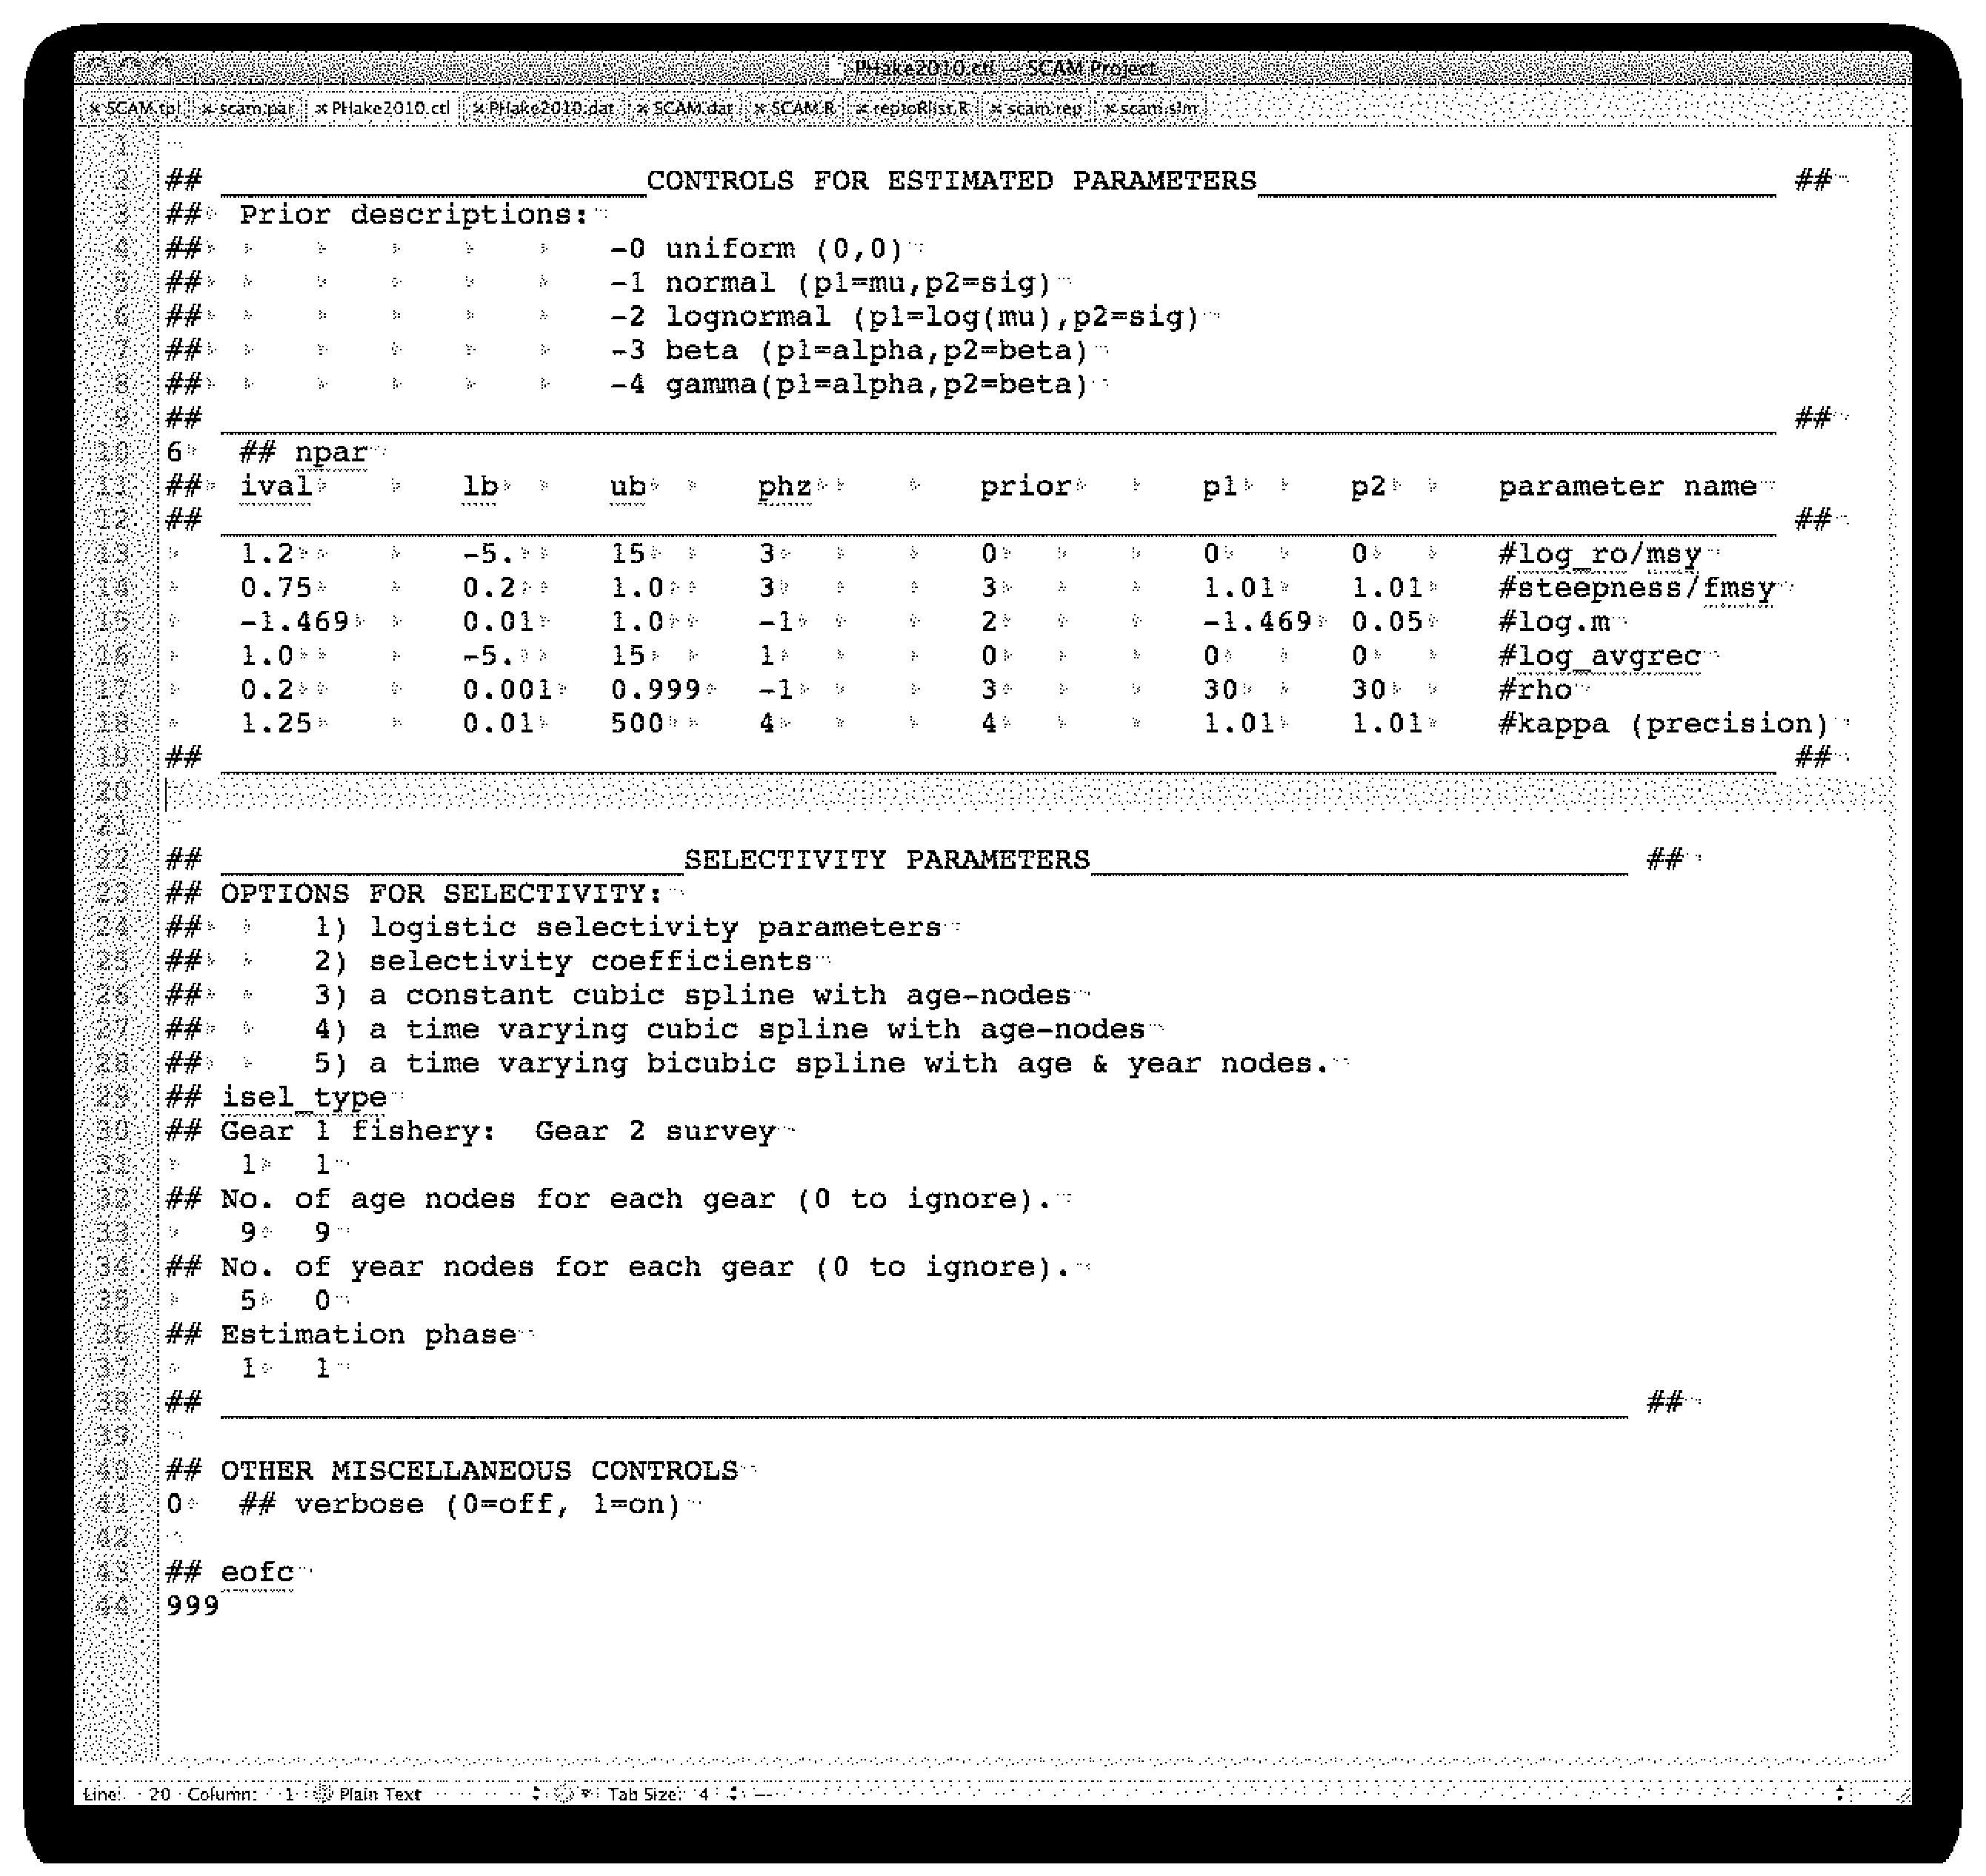
\includegraphics[width=\textwidth]{sc1.eps}\\
%	\caption{A screen shot of the example control file.}\label{Fig.control.file}
%\end{figure*}



\begin{multicols}{2}

\subsection{Command line options}
Currently there are two custom command line options available in \iscam\ in addition to the standard command line options provided by the AD Model Builder libraries (see help command line options -? for more information on the ADMB command line options). 

The custom command line options are:
\begin{description}
\item[-sim N] use this option turn the model into a simulation model, where N is the random number seed.

\item[-retro N] use the option for retrospective analysis where the last N years of data are ignored in the likelihood calculations.
\end{description}

There two random number seeds for the simulation model that the user should be aware of.  The first is if the random number seed is set to 000, then \iscam\ will actually simulate data with no errors whatsoever.  That is, the values of $\sigma$ and $\tau$ (observation error and process errors, respectively) will be set equal to 0 and the simulation model will run as a deterministic model with no observation errors in the relative abundance index or age composition data.  This option allows the user to check to ensure that the model parameters are in fact estimable with perfect information.


The second unique random seed number is 99, and this seed number is used for the simulation example in this manuscript.  It specifies a unique time-varying selectivity curve for the commercial fishery that goes from dome-shaped to asymptotic.

\subsubsection{Running the simulation model}

Again, one of the first steps in conducting any assessment should be to first run the model on simulated data with no error to be certain that the model is capable of estimating the specified model parameters.  To do so in \iscam\, the user simply needs to specify the command line option of \texttt{-sim 000}, where the `000' argument specifically instructs \iscam\ not to add any random variation to the observation or process errors.  Invoking this command line option will run \iscam\ as normal, where the data from the data file is first read into memory, then the information from the control file is then read in.  However, before proceeding straight into the non-linear parameter estimation procedure, \iscam\ first runs a simulation model based on the specified parameters listed in the control file.  This simulation model will then replace the existing data in memory with simulated data, then perform the non-linear parameter estimation procedure and attempt to estimate the model parameters.  If all is working well the estimated parameters listed in the parameter file should be very close, if not exactly, to the initial values specified in the control file.



\end{multicols}

% section running_iscam_input_files_&_command_line_options (end)

%    %!TEX root = /Users/stevenmartell1/Documents/iSCAM-project/docs/iSCAM-guide/userGuide/usrGuide.tex
\section{Model Documentation} % (fold)
\label{sec:model_documentation}

\begin{multicols}{2}

The section contains the documentation in mathematical form of the underlying age-structured model, and its steady state version that is used to calculate reference points, the observation models used in predicting observations, and the components of the objective function that formulate the statistical criterion (i.e., the objective function) that is used to estimate model parameters.  All of the model equations are laid out in tables and are intended to represent the order of operations, or pseudocode, in which to implement the model.  \iscam\ was implemented in AD Model Builder version 10.0 \citep{otterResearch,ADMB2009}.

\subsection{List of symbols} % (fold)
\label{sub:list_of_symbols}
A documented list of symbols for the \iscam program is found in Table~\ref{tab:list_of_symbols} on page~\pageref{tab:list_of_symbols}.

% subsection list_of_symbols (end)


\end{multicols}


% List of symbols
\begin{center}
\begin{longtable}{lll}
\caption[list of symbols]{A list of symbols, constants and description for variables used in \iscam.} 
\label{tab:list_of_symbols} \tabularnewline

\hline 
\multicolumn{1}{l}{\textbf{Symbol}} & 
\multicolumn{1}{l}{\textbf{Value}} & 
\multicolumn{1}{l}{\textbf{Description}} \tabularnewline
\hline 
\endfirsthead

\multicolumn{3}{l}%
{{\bfseries \tablename\ \thetable{} -- continued from previous page}} 
\tabularnewline
\hline 
\multicolumn{1}{l}{\textbf{Symbol}} & 
\multicolumn{1}{l}{\textbf{Value}} & 
\multicolumn{1}{l}{\textbf{Description}} \tabularnewline
\hline 
\endhead

\hline \multicolumn{3}{l}{{Continued on next page}} \tabularnewline
\hline
\endfoot

\hline \hline
\endlastfoot

\multicolumn{3}{l}{\underline{Indexes}}\\
a & & index for age\\
t & & index for year\\
k & & index for gear\\
\multicolumn{3}{l}{\underline{Model dimensions}}\\
$\acute{a}, A$  & 2, 10         & youngest and oldest age class ($A$ is a plus group)\\
$\acute{t}, T$  & 1951, 2010    & first and last year of catch data\\
$K$             & 5             & Number of gears including survey gears\\
\multicolumn{3}{l}{\underline{Observations (data)}}\\
$C_{k,t}$       & & catch in weight by gear $k$ in year $t$\\
$I_{k,t}$       & & relative abundance index for gear $k$ in year $t$\\
$p_{k,t,a}$     & & observed proportion-at-age $a$ in year $t$ for gear $k$\\
\multicolumn{3}{l}{\underline{Estimated parameters}}\\
$R_o$               & & Age-$\acute{a}$ recruits in unfished conditions\\
$\kappa$            & & recruitment compensation\\
$M$                 & & instantaneous natural mortality rate \\
$\bar{R}$           & & average age-$\acute{a}$ recruitment from year $\acute{t}$ to $T$\\
$\ddot{R}$          & & average age-$\acute{a}$ recruitment in year $\acute{t}-1$\\
$\rho$              & & fraction of the total variance associated with observation error\\
$\vartheta$         & & total precision (inverse of variance) of the total error\\
$\vec{\gamma}_k$    & & vector of selectivity parameters for gear $k$\\
$\digamma_{k,t}$    & & logarithm of the instantaneous fishing mortality for gear $k$ in year $t$\\
$\ddot{\omega}_a$   & & age-$\acute{a}$ deviates from $\ddot{R}$ for year $\acute{t}$\\
$\omega_t$          & & age-$\acute{a}$ deviates from $\bar{R}$ for years $\acute{t}$ to $T$\\
$\varphi_t$         & & logarithm of annual change in natural mortality rate\\
\multicolumn{3}{l}{\underline{Standard deviations}}\\
$\sigma_M$          &0.1    & standard deviation in random walk for natural mortality\\
$\sigma$            &       & standard deviation for observation errors in survey index\\
$\tau$              &       & standard deviation in process errors (recruitment deviations)\\
$\sigma_C$          &0.0707 & standard deviation in observed catch by gear\\
\multicolumn{3}{l}{\underline{Residuals}}\\
$\delta_t$      &   & annual recruitment residual\\
$\eta_t$        &   & residual error in predicted catch\\


\end{longtable}
\end{center}


\subsection{Analytic methods: equilibrium considerations} % (fold)
\label{sub:analytic_methods_equilibrium_considerations}

\begin{multicols}{2}
\subsubsection{A steady-state age-structured model} % (fold)
\label{ssub:a_steady_state_age_structured_model}

% subsubsection a_steady_state_age_structured_model (end)

For the steady-state conditions represented in Table~\ref{tab:equilibrium_model}, we assume the parameter vector $\Theta$ in \eqref{T2.1} is unknown and would eventually be estimated by fitting \iscam\ to data.  For a given set of growth parameters and maturity-at-age parameters defined by \eqref{T2.3}, growth is assumed to follow von Bertalanffy \eqref{T2.4}, mean weight-at-age is given by the allometric relationship in \eqref{T2.5}, and the age-specific vulnerability is given by a logistic function \eqref{T2.6}.  Note, however, there are alternative selectivity functions implemented in \iscam, the logistic function used here is simply for demonstration purposes.  Mean fecundity-at-age is assumed to be proportional to the mean weight-at-age of mature fish, where maturity at age is specified by the parameters $\dot{a}$ and $\dot{\gamma}$ for the logistic function.

Survivorship for unfished and fished populations is defined by \eqref{T2.8} and \eqref{T2.9}, respectively.  It is assumed that all individuals ages $A$ and older (i.e., the plus group) have the same total mortality rate.  The incidence functions refer to the life-time or per-recruit quantities such as spawning biomass per recruit ($\phi_E$) or vulnerable biomass per recruit ($\phi_b$).  Note that upper and lower case subscripts denote unfished and fished conditions, respectively.  Spawning biomass per recruit is given by \eqref{T2.10}, the vulnerable biomass per recruit is given by \eqref{T2.11} and the per recruit yield to the fishery is given by \eqref{T2.11b}.  Unfished recruitment is given by \eqref{T2.12} and the steady-state equilibrium recruitment  for a given fishing mortality rate $F_e$ is given by \eqref{T2.13}.  Note that in \eqref{T2.13} we assume that recruitment follows either a  Beverton-Holt or a Ricker model in the forms:
\[
R_e=\begin{cases}
    \dfrac{s_o R_e \phi_e}{1+\beta R_e \phi_e},& \mbox{Beverton-Holt}\\[5ex]
    s_o R_e \phi_e \exp(-\beta R_e \phi_e)& \mbox{Ricker}
\end{cases}
\]
where the maximum juvenile survival rate is the same for both forms of the recruitment model and is given by:
\[
s_o = \kappa/\phi_E,
\]
and the density-dependent term is given by:
\[
\beta =\begin{cases}
    \dfrac{(\kappa-1)}{R_o\phi_E}, & \mbox{Beverton-Holt}\\[5ex]
    {\dfrac {\ln  \left( \kappa \right) }{R_{{o}}\phi_{{E}}}} & \mbox{Ricker}
\end{cases} 
\]
which simplifies to \eqref{T2.13}.
 The equilibrium yield for a given fishing mortality rate is \eqref{T2.14}.  These steady-state conditions are critical for determining various reference points such as \fmsy\ and \bmsy.  



%%%%%%%%%%%%%%%%%%%%%%%%%%%%%%%%%%%%%%%%%%%%%%%%%%%%%%%%%%%%%%%%%%%%%%
%%%%%%%%%%%%%%%%%%%%%%%%%%%%%%%%%%%%%%%%%%%%%%%%%%%%%%%%%%%%%%%%%%%%%%
\begin{tablehere}
  %\centering
\caption{Steady-state age-structured model assuming unequal
vulnerability-at-age, age-specific natural mortality, age-specific
fecundity and Beverton-Holt type recruitment.}\label{tab:equilibrium_model} 
\tableEq
    \begin{gather}
           \hline
        \mbox{Parameters} \nonumber \\
            \Theta = (B_o,\kappa,M_a,\hat{a},\hat{\gamma})      \label{T2.1}\\
            B_o>0; \kappa > 1; M_a > 0\\
            \Phi = (l_\infty, k, t_o,a,b,\dot{a},\dot{\gamma})  \label{T2.3}\\[1ex]
        %%
        %%
        \mbox{Age-schedule information} \nonumber\\
            l_a=l_\infty(1-\exp(-k(a-t_o)))                     \label{T2.4}\\
            w_a=a(l_a)^b                                        \label{T2.5}\\
            v_a=(1+\exp(-(\hat{a}-a)/\gamma))^{-1}              \label{T2.6}\\
            f_a=w_a(1+\exp(-(\dot{a}-a)/\dot{\gamma}))^{-1}     \label{T2.7}\\[1ex]
        %%
        %%
        \mbox{Survivorship} \nonumber\\
            \iota_a=\begin{cases} 1, &\quad a=1                 \label{T2.8}\\
            \iota_{a-1}e^{-M_{a-1}},&\quad a>1\\
            \iota_{a-1}/(1-e^{-M_a}),&\quad a=A \end{cases}\\
            \hat{\iota}_a=\begin{cases} 1, & a=1\\
            \hat{\iota}_{a-1}e^{-M_{a-1}-F_e v_{a-1}},& a>1\\
            \hat{\iota}_{a-1}e^{-M_{a-1}-F_e v_{a-1}}/(1-e^{-M_{a}-F_e v_{a}}),& a=A
            \end{cases}                                         \label{T2.9}\\[1ex]
        %%
        %%
        \mbox{Incidence functions} \nonumber \\
            \phi_E=\sum_{a=1}^\infty \iota_a f_a, \quad
            \phi_e=\sum_{a=1}^\infty \hat{\iota}_a f_a          \label{T2.10}\\
            \phi_B=\sum_{a=1}^\infty \iota_a w_a v_a, \quad
            \phi_b=\sum_{a=1}^\infty \hat{\iota}_a w_a v_a      \label{T2.11}\\
            \phi_q=\sum_{a=1}^\infty
                \frac{ \hat{\iota}_a w_a v_a}{M_a+F_ev_a}
                \left(1-e^{(-M_a-F_ev_a)}\right)                \label{T2.11b}\\[1ex]
        %%
        %%
        \mbox{Steady-state conditions} \nonumber \\
            R_o=B_o/ \phi_B                                     \label{T2.12}\\
            R_e=R_o\begin{cases}
            \dfrac{\kappa-\phi_E/\phi_e}{\kappa-1}&\mbox{Beverton-Holt}\\[2ex]
            \dfrac{\ln(\kappa)-\ln(\phi_E/\phi_e)}{\ln(\kappa)}& \mbox{Ricker}
            \end{cases}                                         \label{T2.13}\\
            C_e=F_e R_e \phi_q                                  \label{T2.14}\\[1ex]
        \hline \hline \nonumber
    \end{gather}
    \normalEq
\end{tablehere}
%%%%%%%%%%%%%%%%%%%%%%%%%%%%%%%%%%%%%%%%%%%%%%%%%%%%%%%%%%%%%%%%%%%%%%
%%%%%%%%%%%%%%%%%%%%%%%%%%%%%%%%%%%%%%%%%%%%%%%%%%%%%%%%%%%%%%%%%%%%%%
 

% subsection sub:analytic_methods_equilibrium_considerations (end)
%!TEX root = /Users/stevenmartell1/Documents/iSCAM-project/docs/iSCAM-guide/userGuide/usrGuide.tex
The concept of maximum sustainable yield, or MSY, is based on the notion that the underlying stock-size versus productivity can be estimated with some degree of certainty, and that this production function is stationary over time.  For a single fishing fleet, this can easily be represented as the equilibrium catch versus the equilibrium fishing effort (Fig. \ref{fig:iscamFigs_Fig1Quadplot}a), hereafter referred to as a yield curve. In the case of multiple fishing fleets, this yield curve  is not necessarily a smooth function as the total yield summed over all fleets is also a function of the fishing mortality exerted by each of the fleets.  In section \ref{ssub:msy_based_reference_points} a description of the equilibrium yields and MSY-based reference points is given, followed by a description of the numerical methods used to obtain MSY-based reference points when there are two or more fleets fishing simultaneously.

A special class library to implement the MSY-based reference point calculations was developed specifically for \iscam.  The C++ code for this class can be found in \texttt{msy.cpp}.


\subsubsection{MSY based reference points: single fleet} % (fold)
\label{ssub:msy_based_reference_points}



In the case of a single fishery \iscam\ calculates \fmsy\ based reference points by finding the value of $F_e$ that results in the zero derivative of \eqref{T2.14}.  This is accomplished numerically using a Newton-Raphson method where an initial guess for \fmsy\ is set equal to 1.0$M$, then use \eqref{eq1.1} to iteratively find \fmsy.  Note that the partial derivatives in \eqref{eq1.1} can be found in Table~\ref{tab:partial_derivatives}.

\begin{align}\label{eq1.1}
    F_{e+1}&=F_e - 
    \dfrac{ \dfrac{\partial C_e}{\partial F_e}}
    { \dfrac{\partial C_e^2}{\partial F_e^2}}\\
    \mbox{where}\nonumber\\
     \frac{\partial C_e}{\partial F_e} &=
    R_e \phi_q
    + F_e \phi_q \dfrac{\partial R_e}{\partial F_e}
    + F_e R_e \dfrac{\partial \phi_q}{\partial F_e} \nonumber\\
    \frac{\partial C_e^2}{\partial F_e^2} &=
    \phi_q \dfrac{\partial R_e}{\partial F_e}
   +  R_e \dfrac{\partial \phi_q}{\partial F_e}\nonumber
%    \frac{R_e \phi_q
%    + F_e \phi_q \dfrac{\partial R_e}{\partial F_e}
%    + F_e R_e \dfrac{\partial \phi_q}{\partial F_e}}
%    {\phi_q \dfrac{\partial R_e}{\partial F_e}
%    +  R_e \dfrac{\partial \phi_q}{\partial F_e}}.
\end{align}

The algorithm usually converges in less than 10 iterations depending on how close the initial guess of \fmsy\ is to the true value.  A maximum of 200 iterations are allowed in \iscam\ and if $\frac{\partial C_e}{\partial F_e}<1e-12$ it is assumed to be sufficiently close to zero and iterations will stop.  Note also, that this class object is only performed on data type variables and not differentiable variables within AD Model Builder.
 

\begin{figurehere}
    \centering
        \includegraphics[height=3in]{iscamFigs/Fig1Quadplot.pdf}
    \caption{Equilibrium yield (a), recruits (b), biomass (c) and
       spawner per recruit ($\phi_e/\phi_E$) (d) versus instantaneous
       fishing mortality $F_e$ for two different values of the recruitment
       compensation ratio ($\kappa=12$ solid lines, $\kappa=4$ dashed
       lines). Vertical lines in each panel correspond to \fmsy\ and
       horizontal lines correspond to various reference points that would
       achieve MSY.}
    \label{fig:iscamFigs_Fig1Quadplot}
\end{figurehere}

Given an estimate of \fmsy, other reference points such as MSY are calculated use the equations in Table-\ref{tab:equilibrium_model} where each of the expressions is evaluated at \fmsy.  A graphical representation of MSY based reference points for two alternative values of the recruitment compensation parameter $\kappa$ is show in Figure \ref{fig:iscamFigs_Fig1Quadplot}. All other parameters in the vectors $\Theta$ and $\Phi$ are identical between the two scenarios.  A lower recruitment compensation ratio (or a lower steepness value in the stock recruitment relationship) implies lower stock productivity or less resilience to fishing. Recruitment and biomass decrease at a much faster rate with increased fishing mortality in comparison to a stock with a higher recruitment compensation ratio. Note that the spawning potential ratio (SPR) curve is insensitive to the estimated value of recruitment compensation (steepness);  however, the SPR value at which MSY is achieved increases with lower recruitment compensation (Fig \ref{fig:iscamFigs_Fig1Quadplot}d).


%%%%%%%%%%%%%%%%%%%%%%%%%%%%%%%%%%%%%%%%%%%%%%%%%%%%%%%%%%%%%%%%%%%%%%
%%%%%%%%%%%%%%%%%%%%%%%%%%%%%%%%%%%%%%%%%%%%%%%%%%%%%%%%%%%%%%%%%%%%%%
\begin{tablehere}
  \centering
\caption{Partial derivatives, based on components in Table
\ref{tab:equilibrium_model}, required for the numerical calculation of \fmsy\ using \eqref{eq1.1}.}\label{tab:partial_derivatives} \tableEq
    \begin{gather}
        \hline
        \mbox{Mortality \& Survival} \nonumber \\
        Z_{a}=M_a+F_ev_a                                \label{T3.1} \\
        S_{a}=1-e^{-Z_a}                                \label{T3.2}\\[1ex]
        %%
        %%
        \mbox{Partial for survivorship} \nonumber \\
        \frac{\partial \hat{\iota}_a}{\partial F_e} =
        \begin{cases}
          0,& a=1                                       \label{T3.3}\\
          e^{-Z_{a-1}}\left(\dfrac{\partial \hat{\iota}_{a-1}}{\partial F_e}
           -\hat{\iota}_{a-1}v_{a-1}\right),& 1<a<A\\
           \dfrac{\dfrac{\partial \hat{\iota}_{a-1}}{\partial F_e}}
           {1-e^{-Z_a}} -
           \dfrac{\hat{\iota}_{a-1} e^{-Z_{a-1}} v_a e^{-Z_a}}
           {(1-e^{-Z_a})^2}, &a=A
        \end{cases} \\[1ex]
%%        \frac{\partial \hat{\iota}_a}{\partial F_e} =
%%        \begin{cases}
%%          0,& a=1 \label{T3.3}\\
%%          e^{-Z_{a-1}}\left(\dfrac{\partial \hat{\iota}_{a-1}}{\partial F_e}
%%           -\hat{\iota}_{a-1}v_{a-1}\right),& a>1
%%        \end{cases} \\[1ex]
        %%
        %%
        \mbox{Partials for incidence functions} \nonumber \\
        \frac{\partial \phi_e}{\partial F_e}=
            \sum_{a=1}^\infty f_a \frac{\partial \hat{\iota}_a}{\partial
            F_e}                                        \label{T3.4}\\
        %%
        %%
        \frac{\partial \phi_q}{\partial F_e}=
            \sum_{a=1}^\infty \frac{w_av_a S_a}{Z_a}
             \frac{\partial \hat{\iota}_a}{\partial F_e}
             +\frac{\hat{\iota}_a w_av_a^2}{Z_a}\left(e^{-Z_a}-\frac{S_a}{Z_a} \right)
                                                            \label{T3.5}\\[1ex]
        %%
        %%
        \mbox{Partial for recruitment} \nonumber\\
        \frac{\partial R_e}{\partial F_e}=\frac{R_o}{\kappa-1}
        \frac{\phi_E}{\phi_e^2} \frac{\partial \phi_e}{\partial
        F_e}                                                \label{T3.6}\\[1ex]
        \hline \hline \nonumber
    \end{gather}

    \normalEq
\end{tablehere}
%%%%%%%%%%%%%%%%%%%%%%%%%%%%%%%%%%%%%%%%%%%%%%%%%%%%%%%%%%%%%%%%%%%%%%
%%%%%%%%%%%%%%%%%%%%%%%%%%%%%%%%%%%%%%%%%%%%%%%%%%%%%%%%%%%%%%%%%%%%%%

% subsubsection msy_based_reference_points (end)

\subsubsection{MSY Based Reference Points: two or more fleets} % (fold)
\label{ssub:msy_based_reference_points_two_or_more_fleets}

In the case where there are two or more fishing fleets with distinctly different selectivity curves for each of the fleets, determination \fmsy for each of the fleets is a bit more complicated.  The first major complication is solving the catch equation where \eqref{T2.14} now involves a summation term over different fishing fleets.  The second complication is how should the total catch (summed over fleets) be allocated to each of the fleets.  In the special case where selectivity for each of the fishing fleets is identical, an equal proportion of the total catch allocated to each of those fleets also corresponds to the same fishing mortality for each of those fleets.  In the more common case where selectivity differs among fleets, the fishing mortality rates associated with equal allocations would also differ.  Consider the following example, if you have a purse seine fleet that harvests small young tuna, and a long-line fleet that harvest the same stock but selects larger older tuna. If each of these two fleets are allocated a 50:50 share, the instantaneous fishing mortality rate would have to be much higher for the long-line gear relative to the purse seine gear that harvest the more abundance small/young tuna.  Regarding the first complication, the following description is based on the assumption is that the total catch summed over all fleets is maximized, and that allocation of total catch is a secondary issue. For the second complication, a vector of fishing mortality rate multipliers is used to adjust fleet specific fishing mortality rates to satisfy catch allocations.  Lastly, a third complication pertains to the accounting of mature numbers-at-age at the time of spawning and how much of the total annual mortality occurs prior to spawning. 


% From msy.cpp
The steady-state catch equation for fleet $k$, with an instantaneous fishing mortality rate $F_k$, is given by:
\begin{align}
	C_{k} &= F_k R_e \phi_{q,k} \label{eq:C_k}\\
	\mbox{where}\nonumber\\
	R_e &= \frac{R_o (\kappa-\phi_E/\phi_e)}{\kappa-1} \label{eq:R_e}\\  %ro*(kappa-m_phie/phif) / km1;
	\phi_{q,k} &= \sum_j = \frac{e^{-M(j-1)}V_{k,j}w_a (1-e^{-M-\sum_k F_k V_{k,j} })}{M+\sum_k F_k V_{k,j}} \label{eq:phi_qk}
\end{align}

Although the catch equation appears relatively simple, there are two key points to note about the equilibrium recruitment $R_e$ and the yield per recruit $\phi_{q,k}$ in \eqref{eq:R_e} and \eqref{eq:phi_qk}, respectively. First, \eqref{eq:R_e} is a function of the eggs per recruit under fished conditions $\phi_e$, which is based on the survivorship which depends on the fishing mortality rates of all gears.  Second, the yield per recruit in \eqref{eq:phi_qk} is a function of the total mortality rate which involves the summation over gears.

The maximum total yield summed over all $k$ fleets occurs under the following condition:
\begin{equation}
	0 = \sum_k \frac{\partial C_k}{\partial F_k}  \label{eq:Catch_derivative}
\end{equation}
and thus the goal is to find a vector of steady-state fishing mortality rates $F_k$ to satisfy \eqref{eq:Catch_derivative}.  


% subsubsection msy_based_reference_points_two_or_more_fleets (end)


\subsubsection{Reference points for multiple fisheries with fixed allocation} % (fold)
\label{ssub:reference_points_for_multiple_fisheries}
% It is common that a single stock of fish is prosecuted by many different types of fishing gears that have differing selectivities.  In such cases, the definition of MSY is based on the sum of catches from each of the participating fleets and how much of the total catch is taken, or allocated, to specific sectors.  For such cases, it is still possible to calculate MSY-based reference points provided that allocation to each of the gear types is specified \emph{a priori}.

To determine MSY-based reference points for 2 or more gear types (e.g.,  purse seine and gillnet fisheries for Pacific herring in British Columbia), \iscam\ requires an allocation for each of the defined fleets.  Allocation is specified in the data file (see sub section \ref{sub:the_data_file}).  This allocation is initially used set a series of F-multipliers ($\lambda_k$) for each gear and \eqref{T2.14} becomes a vector of catches:
\begin{align}
	C_{e,k} &= F_e \lambda_k R_e \phi_{q,k} \label{eq:12} \\
	&\mbox{where the per-recruit yield for gear $k$ is:} \nonumber \\
	Z_a &= M+F_e\sum_k \lambda_kv_{k,a}\label{eq:13}\\
	\phi_{q,k}&=\sum_{a=1}^\infty
        \frac{ \hat{\iota}_a \lambda_k w_a v_{k,a}}{Z_a}
        \left(1-e^{Z_a}\right)\label{eq:14}\\
    &\mbox{with the added constraint} \nonumber\\
    \sum_k \lambda_k &= N \label{eq:15}\quad \mbox{where $N$ is the number of gears.}
\end{align}

The constraint in \eqref{eq:15} defines $F_e\lambda_k$ as the fishing mortality rate for gear $k$ where $\lambda_k$ is a multiple of the average fishing mortality rate of all gears.  To ensure that each gear achieves the specified allocation for a given average fishing mortality rate $F_e$, the multipliers are determined iteratively where $\lambda_k$ is updated using:
\begin{align}
	\lambda_k^{(i+1)} &= \lambda_k^{(i)} \frac{a_k}{p_k} \label{eq:16}\\
	&\mbox{where $a_k$ is the allocation for gear $k$, and:}\nonumber\\
	p_k &= \frac{C_{e,k}}{\sum_k C_{e,k}}\label{eq:17}
\end{align}
Depending on the differences in selectivities and allocations between the gear types, this algorithm converges roughly 7-15 iterations.  From here the same Newton-Raphson algorithm is used to determine the average fishing mortality rate $F_e$ that would maximize the sum of catches over the multiple gears.  
% subsubsection reference_points_for_multiple_fisheries (end)



\subsection{MSY-based reference points for multiple fisheries} % (fold)
\label{sub:msy_based_reference_points_for_multiple_fisheries}

In cases where there are two or more fishing fleets that harvest the same stock (intentionally or taken as bycatch), the differences in selectivity among these gears will ultimately affect the fishing mortality rates associated with long-term sustainable yields or MSY for each of the participating fleets.  For example, global tuna fisheries are taken primarily by two gear types, pelagic longlines which harvest larger/older tuna, and purse seine's which harvest younger tuna usually aggregated around Fish Aggregating Devices (FADs).  The longline fishery has been in operation since the 1950s (even longer, but the available data date back to the 1950s), and the industrial purse seine fishery developed in the 1980s.  If in fact the longline fishery was fully utilized by the 1980s, then the impacts of increased mortality on younger tuna from the purse seine fleet would reduce the available surplus for the longline fishery.

To estimate what the appropriate MSY-based fishing mortality rates for two or more fishing gears that harvest the same stock of fish, the catch equations for each fleet must be simultaneously solved in order to find the appropriate vector of fishing mortality rates that that maximizes the yields for each fleet.  The steady-state, or equilibrium, catch equation for a given fishing gear $k$ is given by:
\begin{equation}\label{eq:equilYield}
	 Y_{k} = \sum_j\frac{N_j F_k v_{k,j} w_j (1-\exp(-M-\sum_k F_k v_{k,j}))} {M + \sum_k F_k v_{k,j}},
\end{equation}
where $F_k$ is the fishing mortality rate imposed by gear $k$, M is the instantaneous natural mortality rate, $v_{k,j}$ is the age-specific selectivity for gear $k$ and age $j$, and $w_j$ and $N_j$ are the average weight-at-age and numbers-at-age, respectively.  Note that if $k>1$, then \eqref{eq:equilYield} represents of system of nonlinear equations where the roots of these equations $\left(\frac{\partial Y_k}{\partial F_k}=0\right)$ are found with Newton-Raphson.

\subsubsection{Algorithm for estimating \fmsy\ for multiple fleets} % (fold)
\label{ssub:algorithm_for_estimating_fmsy_for_multiple_fleets}


% subsubsection algorithm_for_estimating_fmsy_for_multiple_fleets (end)

% subsection msy_based_reference_points_for_multiple_fisheries (end)





\end{multicols}




\subsection{Analytic methods: state-dynamics} % (fold)
\label{sub:analytic_methods_state_dynamics}


\begin{multicols}{2}
The estimated parameter vector in \iscam\ is defined in \eqref{T4.1}, where $R_0, \kappa$ and $M$ are the leading unknown population parameters that define the overall population scale in the form of unfished recruitment and productivity in the form of recruitment compensation and natural mortality.  The total variance $\vartheta^2$ and the proportion of the total variance that is associated with observation errors $\rho$ are also estimated, then the variance is partitioned into observation errors ($\sigma^2$) and process errors ($\tau^2$) using \eqref{T4.2}.

The unobserved state variables \eqref{T4.3} include the numbers-at-age year year $t$ ($N_{t,a}$), the spawning stock biomass ($B_t$) and the total age-specific total mortality rate ($Z_{t,a}$).

The initial numbers-at-age in the first year \eqref{T4.4} and the annual recruits \eqref{T4.5} are treated as estimated parameters and used to initialize the numbers-at-age matrix.  Age-specific selectivity for gear type $k$ is a function of the selectivity parameters $\gamma_k$ \eqref{T4.6}, and the annual fishing mortality for each gear $k$ in year $t$ ($\digamma_{k,t}$).  The vector of log fishing mortality rate parameters $\digamma_{k,t}$ is a bounded vector with a minimum value of -30 and an upper bound of 3.0.  In arithmetic space this corresponds to a minimum value of 9.36e-14 and a maximum value of 20.01 for annual fishing mortality rates.  In years where there are 0 reported catches for a given fleet, no corresponding fishing mortality rate parameter is estimated and the implicit assumption is there was no fishery in that year.

There is an option to treat natural mortality as a random walk process \eqref{T4.6b}, where the natural mortality rate in the first year is the estimated leading parameter \eqref{T4.1} and in subsequent years the mortality rate deviates from the previous year based on the estimated deviation parameter $\varphi_t$.  If the mortality deviation parameters are not estimated, then $M$ is assumed to be time invariant.

State variables in each year are updated using equations \ref{T4.8}--\ref{T4.11}, where the spawning biomass is the product of the numbers-at-age and the mature biomass-at-age \eqref{T4.8}.  The total mortality rate is given by \eqref{T4.9}, and the total catch (in weight) for each gear is given by \eqref{T4.10} assuming that both natural and fishing mortality occur simultaneously throughout the year.  The numbers-at-age are propagated over time using \eqref{T4.11}, where members of the plus group (age $A$) are all assumed to have the same total mortality rate.  

Recruitment to age $k$ can follow either a Beverton-Holt model \eqref{T4.12} or a Ricker model \eqref{T4.13} where the maximum juvenile survival rate ($s_o$) in either case is defined by $s_o=\kappa/\phi_E$.  For the Beverton-Holt model, $\beta$ is derived by solving \eqref{T4.12} for $\beta$ conditional on estimates of $\kappa$ and $R_o$:
\[
\beta = \frac{\kappa-1}{R_o \phi_E},
\]
and for the Ricker model this is given by:
\[
\beta = \frac{\ln(\kappa)}{R_o \phi_E}
\]

%%%%%%%%%%%%%%%%%%%%%%%%%%%%%%%%%%%%%%%%%%%%%%%%%%%%%%%%%%%%%%%%%%%%%%%%
%%%%%%%%%%%%%%%%%%%%%%%%%%%%%%%%%%%%%%%%%%%%%%%%%%%%%%%%%%%%%%%%%%%%%%%%
\begin{tablehere}
  \centering
\caption{Statistical catch-age model using the Baranov catch.}
\label{tab:statistical_catch_age_model}
\tableEq
    \begin{align}
        \hline \nonumber \\
        &\mbox{Estimated parameters} \nonumber\\
        \begin{split}
        \Theta&= 
                (R_0,\kappa,M,\bar{R},\rho,\vartheta^2,\gamma_{k},%\bar{F}_k,
                \digamma_{k,t},\\
        &\quad \{\omega_t\}_{t=1-A}^{t=T},
                \{\varphi_t \}_{t=2}^T)
    \end{split} \label{T4.1}\\
        \sigma^2&=\rho /\vartheta^2, \quad
        \tau^2=(1-\rho)/\vartheta^2\label{T4.2}\\[1ex]
        %\vartheta^2=\sigma^2+\tau^2, \quad
        %\rho=\frac{\sigma^2}{\sigma^2+\tau^2}\label{T4.3}\\[1ex]
        %%
        %%
        &\mbox{Unobserved states} \nonumber\\
        &N_{t,a},B_t,Z_{t,a}    \label{T4.3}\\
    %%
    %%          
        &\mbox{Initial states} \nonumber\\
        %v_a=\left[1+e^{-(\hat{a}-a)/\hat{\gamma}}\right]^{-1}\label{T4.7}\\
        N_{t,a}&=\bar{R}e^{\omega_{t-a}} \exp(-M_t)^{(a-1)};\quad t=1;  2\leq a\leq A \label{T4.4}\\
        N_{t,a}&=\bar{R}e^{\omega_{t}} ;\quad 1\leq t\leq T;  a=1 \label{T4.5}\\
        v_{k,a}&=f(\gamma_k) \label{T4.6}\\
        M_t &= M_{t-1} \exp(\varphi_t), \quad t>1 \label{T4.6b}\\
        F_{k,t}&=\exp(\digamma_{k,t}) \label{T4.7}\\[1ex]
        %%
        %%
        &\mbox{State dynamics (t$>$1)} \nonumber\\
        B_t&=\sum_a N_{t,a}f_a \label{T4.8}\\
        Z_{t,a}&=M_t+\sum_k F_{k,t} v_{k,t,a}\label{T4.9}\\
        \hat{C}_{k,t}&=\sum _ a\frac {N_{{t,a}}w_{{a}}F_{k,t} v_{{k,t,a}}
        \left( 1-{e^{-Z_{t,a}}} \right) }{Z_{t,a}}^{\eta_t} \label{T4.10}\\
        %F_{t_{i+1}}= \ F_{t_{i}} -\frac{\hat{C}_t-C_t}{\hat{C}_t'} \label{T4.12}\\
        N_{t,a}&=\begin{cases}
            %\dfrac{s_oE_{t-1}}{1+\beta E_{t-1}} \exp(\omega_t-0.5\tau^2) &a=1\\ \\
            N_{t-1,a-1} \exp(-Z_{t-1,a-1}) &a>1\\
            N_{t-1,a} \exp(-Z_{t-1,a}) & a=A
        \end{cases}\label{T4.11}\\[1ex]
        %%
        %%
        &\mbox{Recruitment models} \nonumber\\
        R_t &= \frac{s_oB_{t-k}}{1+\beta B_{t-k}}e^{\delta_{t}-0.5\tau^2} \quad \mbox{Beverton-Holt} \label{T4.12}\\
        R_t &= s_oB_{t-k}e^{-\beta B_{t-k}+\delta_t-0.5\tau^2} \quad \mbox{Ricker} \label{T4.13}\\
    %%        \mbox{Residuals \& predicted observations} \nonumber\\
    %%        \epsilon_t=\ln\left(\frac{I_t}{B_t}\right)-\frac{1}{n}\sum_{t \in I_t}\ln\left(\frac{I_t}{B_t}\right)\label{T4.15}\\
    %%        \hat{A}_{t,a}=\dfrac{N_{t,a}\dfrac{F_tv_a}{Z_{t,a}}\left(1-e^{-Z_{t,a}}\right)}
    %%        {\sum_a N_{t,a}\dfrac{F_tv_a}{Z_{t,a}}\left(1-e^{-Z_{t,a}}\right)}\label{T4.16}\\
        \hline \hline \nonumber
    \end{align}

    \normalEq
\end{tablehere}
%%%%%%%%%%%%%%%%%%%%%%%%%%%%%%%%%%%%%%%%%%%%%%%%%%%%%%%%%%%%%%%%%%%%%%%%
%%%%%%%%%%%%%%%%%%%%%%%%%%%%%%%%%%%%%%%%%%%%%%%%%%%%%%%%%%%%%%%%%%%%%%%%





\subsubsection{Options for selectivity ($v_{k,t,a}$)} \label{ModelDocSelectivity}

At present, there are six alternative age-specific selectivity options in \iscam.  The simplest of the selectivity options is a simple logistic function with two parameters where it is assumed that selectivity is time-invariant.  The more complex selectivity options assume that selectivity may vary over time a may have as many as (A-1)$\cdot$T parameters.  For time-varying selectivity, cubic and bicubic splines are used to reduce the number of estimated parameters.  Prior to parameter estimation, \iscam\ will determine the exact number of selectivity parameters that need to be estimated based on which selectivity option was chosen for each gear type.  It is not necessary for all gear types to have the same selectivity option.  For example it is possible to have a simple two parameter selectivity curve for say a survey gear, and a much more complicated selectivity option for a commercial fishery.

\paragraph{Logistic selectivity} 
The logistic selectivity option is a two parameter model of the form
\[
v_a = \frac{1}{1+ \exp{(-(a-\mu_{a})/\sigma_a)}}
\]
where $\mu_a$ and $\sigma_a$ are the two estimated parameters representing the age-at-50\% vulnerability and the standard deviation, respectively.

\paragraph{Age-specific selectivity coefficients}
The second option also assumes that selectivity is time-invariant and estimates at total of $A$-1 selectivity coefficients, where the plus group age-class is assumed to have the same selectivity as the previous age-class.  For example, if the ages in the model range from 1 to 15 years, then a total of 14 selectivity parameters are estimated, and age-15+ animals will have the same selectivity as age-14 animals.

When estimating age-specific selectivity coefficients, there are two additional penalties that are added to the objective function that control how much curvature there is and limit how much dome-shaped can occur.  To penalize the curvature, the square of the second differences of the vulnerabilities-at-age are added to the objective function: 
\[
\lambda_k^{(1)} \sum_{a=2}^{A-1}(v_{k,a} - 2v_{k,a-1} + v_{k,a-2})^2
\]
The dome-shaped term penalty as:
\[
\begin{cases}
\lambda_k^{(2)} \sum_{a=1}^{A-1}(v_{k,a} - v_{k,a+1})^2& \mbox(if) v_{k,a+1}< v_{k,a}\\
0 & \mbox(if) v_{k,a+1}\geq v_{k,a}
\end{cases}
\]
For this selectivity option the user must specify the relative weights ($\lambda_k^{(1)},\lambda_k^{(2)}$) to add to these two penalties.

\paragraph{Cubic spline interpolation}
The third option also assumes time-invariant selectivity and estimates a selectivity coefficients for a series age-nodes (or spline points) and uses a natural cubic spline to interpolate between these nodes (Figure \ref{Fig2}). Given $n+1$ distinct knots $x_i$, selectivity can be interpolated in the intervals defined by
\[
S(x) = \begin{cases}
    S_0(x) & x \in [x_0,x_1]\\
    S_1(x) & x \in [x_1,x_2]\\
    ...\\
    S_{n-1}(x) & x \in [x_{n-1},x_n]
\end{cases}
\]
where  $S''(x_0) = S''(x_n)=0$  is the condition that defines a natural cubic spline.
\begin{figurehere}
    \centering
    % Requires \usepackage{graphicx}
    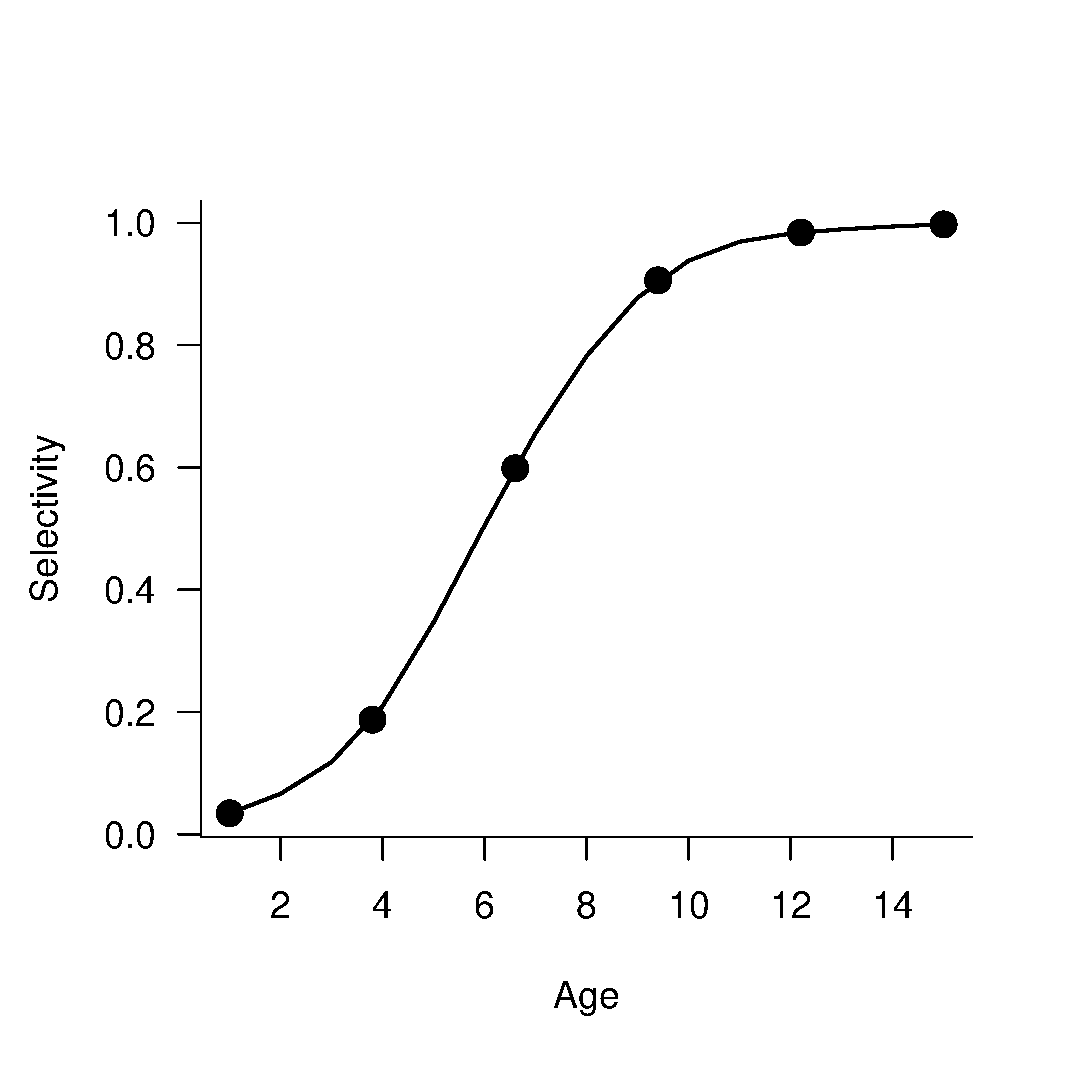
\includegraphics[width=\columnwidth]{iscamFigs/SplineEg.eps}\\
    \caption{Example of a natural cubic spline interpolation for estimating selectivity coefficients.  In \iscam\ the user specifies the number of nodes (circles) to estimate; then age-specific selectivity coefficients are interpolated using a natural cubic spline.}\label{Fig2}
\end{figurehere}

The same penalty functions for curvature and dome-shaped selectivity are also invoked for the cubic spline interpolation of selectivity.

\paragraph{Time-varying selectivity with cubic spline interpolation} A fourth option allows for cubic spline interpolation for age-specific selectivity  in each year.  This option adds a considerable number of estimated parameters but the most extreme flexibility.  For example, given 40 years of data and estimated 5 age nodes, this amounts 200 (40 years times 5 ages) estimated selectivity parameters.  Note that the only constraints at this time are the dome-shaped penalty and the curvature penalty; there is no constraint implemented for say a random walk (first difference) in age-specific selectivity).  As such this option should only be used in cases where age-composition data is available for every year of the assessment.

\paragraph{Bicubic spline to interpolate over time and ages}  The fifth option allows for a two-dimensional interpolation using a bicubic spline (Figure \ref{Fig3}).  In this case the user must specify the number of age and year nodes.  Again the same curvature and dome shaped constraints are implemented.  It is not necessary to have age-composition data each and every year as in the previous case, as the bicubic spline will interpolate between years.  However, it is not advisable to extrapolate selectivity back in time or forward in time where there are no age-composition data unless some additional constraint, such as a random-walk in age-specific selectivity coefficients is implemented (as of \today, this has not been implemented).

\begin{figure*}[!tbp]
    % Requires \usepackage{graphicx}
    \centering
    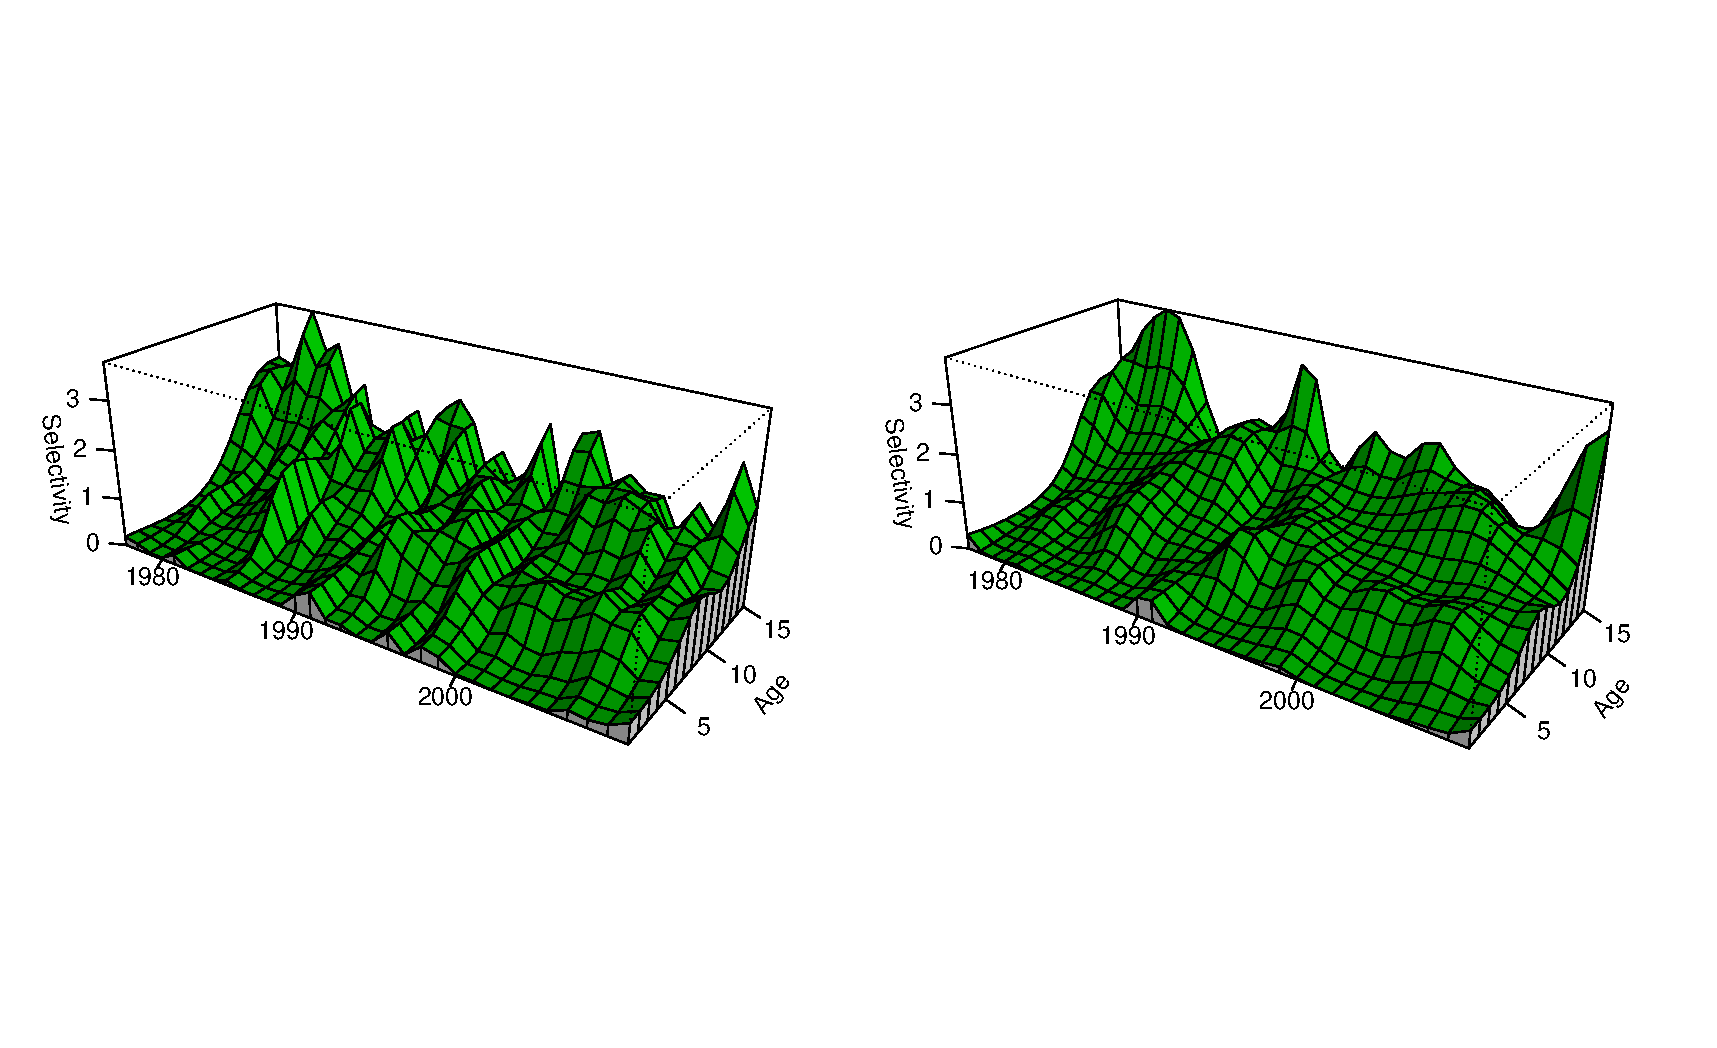
\includegraphics[width=0.9\textwidth]{iscamFigs/BicubicEg.eps}\\
    \caption{Example of a time-varying cubic spline (left) and bicubic spline (right) interpolation for selectivity as applied to the Pacific hake data. The panel on the left contains 165 estimated selectivity parameters and the bicubic interpolation estimates 85 selectivity parameters, or 5 age nodes and 17 year nodes. There are 495 actual nodes being interpolated.}\label{Fig3}
\end{figure*}
%\end{multicols}

\subsection{Residuals, likelihoods \& objective function value components}
%\begin{multicols}{2}
There are 3 major components to the overall objective function that are minimized while \iscam\ is performing maximum likelihood estimation.  These components consist of the likelihood of the data, prior distributions and penalty functions that are invoked to regularize the solution during intermediate phases of the non-linear parameter estimation.  This section discusses each of these in turn, starting first with the residuals between observed and predicted states followed by the negative loglikelihood that is minimized.

\subsubsection{Catch data}
It is assumed that the measurement errors in the catch observations are log-normally distributed, and the residuals is given by:
\begin{equation}\label{eq2}
\eta_{k,t}=\ln(C_{k,t}+o) -  \ln(\hat{C}_{k,t}+o),
\end{equation}
where $o$ is  a small constant (1.e-10) to ensure the residual is defined in the case of a 0 catch observation.  The residuals are assumed to be normally distributed with a user specified standard deviation $\sigma_{C}$.  At present, it is assumed that observed catches for each gear $k$ is assumed to have the same standard deviation.  To aid in parameter estimation, two separate standard deviations are specified in the control file: the first is the assumed standard deviation used in the first, second, to N-1 phases, and the second is the assumed standard deviation in the last phase.  The negative loglikelihood (ignoring the scaling constant) for the catch data is given by:
\begin{equation}\label{eq3}
\ell_C = \sum_k\left[  T_k\ln(\sigma_C)+\frac{\sum_t(\eta_{k,t})^2}{2\sigma_C^2}\right],
\end{equation}
where $T_k$ is the total number of catch observations for gear type $k$.


\subsubsection{Relative abundance data}
The relative abundance data are assumed to be proportional to biomass that is vulnerable to the sampling gear:
\begin{equation}\label{eq4}
 V_{k,t} = \sum_a N_{t,a} e^{-\lambda_{k,t} Z_{t,a}} v_{k,a} w_a,
\end{equation}
where $v_{k,a}$ is the age-specific selectivity of gear $k$, and $w_a$ is the mean-weight-at-age. A user specified fraction of the total mortality $\lambda_{k,t}$ adjusts the numbers-at-age to correct for survey timing.  The residuals between the observed and predicted relative abundance index is given by:
\begin{equation}\label{eq5}
\epsilon_{k,t} = \ln(I_{k,t}) - \ln(q_k)+\ln(V_{k,t}),
\end{equation}
where $I_{k,t}$ is the observed relative abundance index, $q_k$ is the catchability coefficient for index $k$, and $V_{k,t}$ is the predicted vulnerable biomass at the time of sampling.  The catchability coefficient $q_k$ is evaluated at its conditional maximum likelihood estimate:
\[
  q_k =\frac{1}{N_k} \sum_{t \in I_{k,t}} \ln(I_{k,t}) - \ln(V_{k,t}),
\]
where $N_k$ is the number of relative abundance observations for index $k$ \citep[see][for more information]{walters1994calculation}. The negative loglikelihood for relative abundance data is given by:
\begin{align}
\ell_I &= \sum_k \sum_{t \in I_{k,t}}  \ln(\sigma_{k,t})+\frac{\epsilon_{k,t}^2}{2\sigma_{k,t}^2} \label{eq6}\\
&\mbox{where}\nonumber\\
\sigma_{k,t} &= \frac{\rho \varphi^2}{ \omega_{k,t}},  \nonumber
\end{align}
where $\rho \varphi^2$ is the proportion of the total error that is associated with observation errors, and $\omega_{k,t}$ is a user specified relative weight for observation $t$ from gear $k$.  The $ \omega_{k,t}$ terms allow each observation to be weighted relative to the total error $\rho \varphi^2$; for example, to omit a particular observation, set $\omega_{k,t}=0$, or to give 2 times the weight, then set  $\omega_{k,t}=2.0$. To assume all observations have the same variance then simply set  $\omega_{k,t}=1$.  Note that if  $\omega_{k,t}=0$ then equation \eqref{eq6} is undefined; therefore, \iscam\ adds a small constant to  $\omega_{k,t}$ (1.e-10, which is equivalent to assuming an extremely large variance)  to ensure the likelihood can be evaluated.

\subsubsection{Age composition data}\label{agecomps}
Sampling theory suggest that age composition data are derived from a multinomial distribution \citep{fournier1982general}; however, \iscam\ assumes that age-proportions are obtained from a multivariate logistic distribution \citep{schnute1995influence,richards1997visualizing}.  The main reason \iscam\ departs from the traditional multinomial model has to do with how the age-composition data are weighted in the objective function.  First, the multinomial distribution requires the specification of an effective sample size; this may be done arbitrarily or through iterative re-weighting \citep{MCALLISTER1997,gavaris2002sif}, and in the case of multiple and potentially conflicting age-proportions this procedure may fail to converge properly.  The assumed effective sample size can have a large impact on the overall model results.  

A nice feature of the multivariate logistic distribution is that the age-proportion data can be weighted based on the conditional maximum likelihood estimate of the variance in the age-proportions.  Therefore, the contribution of the age-composition data to the overall objective function is ``self-weighting'' and is conditional on other components in the model.

Ignoring the subscript for gear type for clarity, the observed and predicted proportions-at-age must satisfy the constraint 
\[
 \sum_{a=1}^A p_{t,a} = 1
\]
for each year. The residuals between the observed ($p_{t,a}$) and predicted proportions ($\widehat{p_{t,a}}$) is given by:
\begin{equation}\label{eq7}
\eta_{t,a}=\ln(p_{t,a})-\ln(\widehat{p_{t,a}})-\frac{1}{A}\sum_{a=1}^A\left[\ln(p_{t,a})-\ln(\widehat{p_{t,a}}) \right].
\end{equation}
The conditional maximum likelihood estimate of the variance is given by
\[
\widehat{\tau}^2=\frac{1}{(A-1)T}\sum_{t=1}^T\sum_{a=1}^A \eta_{t,a}^2,
\]
and the negative loglikelihood evaluated at the conditional maximum likelihood estimate of the variance is given by:
\begin{equation}\label{eq8}
    \ell_A = (A-1)T \ln(\widehat{\tau}^2).
\end{equation}
In short, the multivariate logistic likelihood for age-composition data is just the log of the residual variance weighted by the number observations over years and ages.

%Add technical details about requiring the minimum p_{t,a} to be greater than 2% "Grouping".
There is also a technical detail in \eqref{eq7}, where observed and predicted proportions-at-age must be greater than 0.  It is not uncommon in catch-age data sets to observe 0 proportions for older, or young, age classes.  \iscam\ adopts the same approach described by \cite{richards1997visualizing} where the definition of age-classes is altered to require that $p_{t,a}\geq 0.02$ for every age in each year.  This is accomplished by grouping consecutive ages, where $p_{t,a} <0.02$, into a single age-class and reducing the effective number of age-classes in the variance calculation ($\widehat{\tau}^2$) by the number of groups created.  The choice of 2\% is arbitrary and the user can specify the minimum proportion (including 0) to consider when pooling age-proportion data.  In the case of an exact 0 in the observed age-proportions the pooling of the adjacent age-class still occurs, this ensures that \eqref{eq7} is defined.


A \textbf{WARNING} about extremely weak year classes is required here.  A potential problem exists if in fact there is a very small cohort relative to the adjacent cohorts such that it never makes up more than say 2\% (or whatever minimum is specified) of the age-proportions in any given year.  In such cases, the information in the age-composition data about this weak year class relative to of that the adjacent (younger) year class because its always pooled into the younger year class.  \iscam\ will actually estimate two strong cohorts instead of correctly estimating one strong and one weak cohort in the following year.

\subsubsection{Stock-recruitment}
There are two alternative stock-recruitment models available in \iscam: the Beverton-Holt model and the Ricker model.  Annual recruitment and the initial age-composition are treated as latent variables in \iscam, and residuals between estimated recruits and the deterministic stock-recruitment models are used to estimate unfished spawning stock biomass and recruitment compensation.  The residuals between the estimated and predicted recruits is given by
\begin{equation}\label{eq9}
    \delta_t = \ln(\bar{R}e^{w_t}) - f(B_{t-k})
\end{equation}
where $f(B_{t-k})$ is given by either \eqref{T4.12} or \eqref{T4.13}, and $k$ is the age at recruitment.  Note that a bias correction term for the lognormal process  errors is included in  \eqref{T4.12} and \eqref{T4.13}.

The negative log likelihood for the recruitment deviations is given by the normal density (ignoring the scaling constant):
\begin{equation}\label{eq10}
 \ell_\delta = n\ln(\tau) + \frac{\sum_{t=1+k}^T \delta^2_t}{2\tau^2}
\end{equation}
Equations \eqref{eq9} and \eqref{eq10} are key for estimating unfished spawning stock biomass and recruitment compensation via the recruitment models.  The relationship between ($s_o,\beta$) and ($B_o,\kappa$) is defined as:
\begin{align}
s_o &= \kappa/\phi_E\\
\beta&=\begin{cases}
\frac{\kappa-1}{B_o} \quad \mbox{Beverton-Holt}\\[1ex]
\frac{\ln(\kappa)}{B_o} \quad \mbox{Ricker}
\end{cases}
\end{align}
where $s_o$ is the maximum juvenile survival rate, and $\beta$ is the density effect on recruitment.



\end{multicols}
% subsection analytic_methods_state_dynamics (end)
% section model_documentation (end)
% \clearpage

    
%    %!TEX root = /Users/stevenmartell1/Documents/iSCAM-project/docs/iSCAM-guide/userGuide/usrGuide.tex


% 
% \section{Example: Simulation based on Strait of Georgia Pacific herring}
% \begin{multicols}{2}
% 
% \subsection{Introduction \& purpose}
% The purpose of this example is to demonstrate how to use \iscam\ to simulate data with known parameter values and then demonstrate the ability of the model to estimate the unknown parameters with and without observation and process errors.  This example is based on data from the Strait of Georgia Pacific herring fishery.
% 
% There are three distinct commercial fishing fleets for Pacific herring in the Strait of Georgia that have operated, and continue to operate, between 1951 and 2010 (Figure \ref{pHerringFig1}).  The first of these fleets is a purse seine fishery that generally operates in the winter months and historically used to catch herring for a reduction fishery and since the 1970s is now a much smaller bait fishery operation.  Since the early 1970s a much more valuable seine fishery for sac roe has been in operation along with a gill net fishery that also targets spawning female herring for its roe.
% 
% \begin{figurehere}
% 	% Requires \usepackage{graphicx}
% 	%\psfrag{Catch (t)}[][c]{Catch (1000 mt)}
% 	%\psfrag{Year}[][c]{Year}
% 	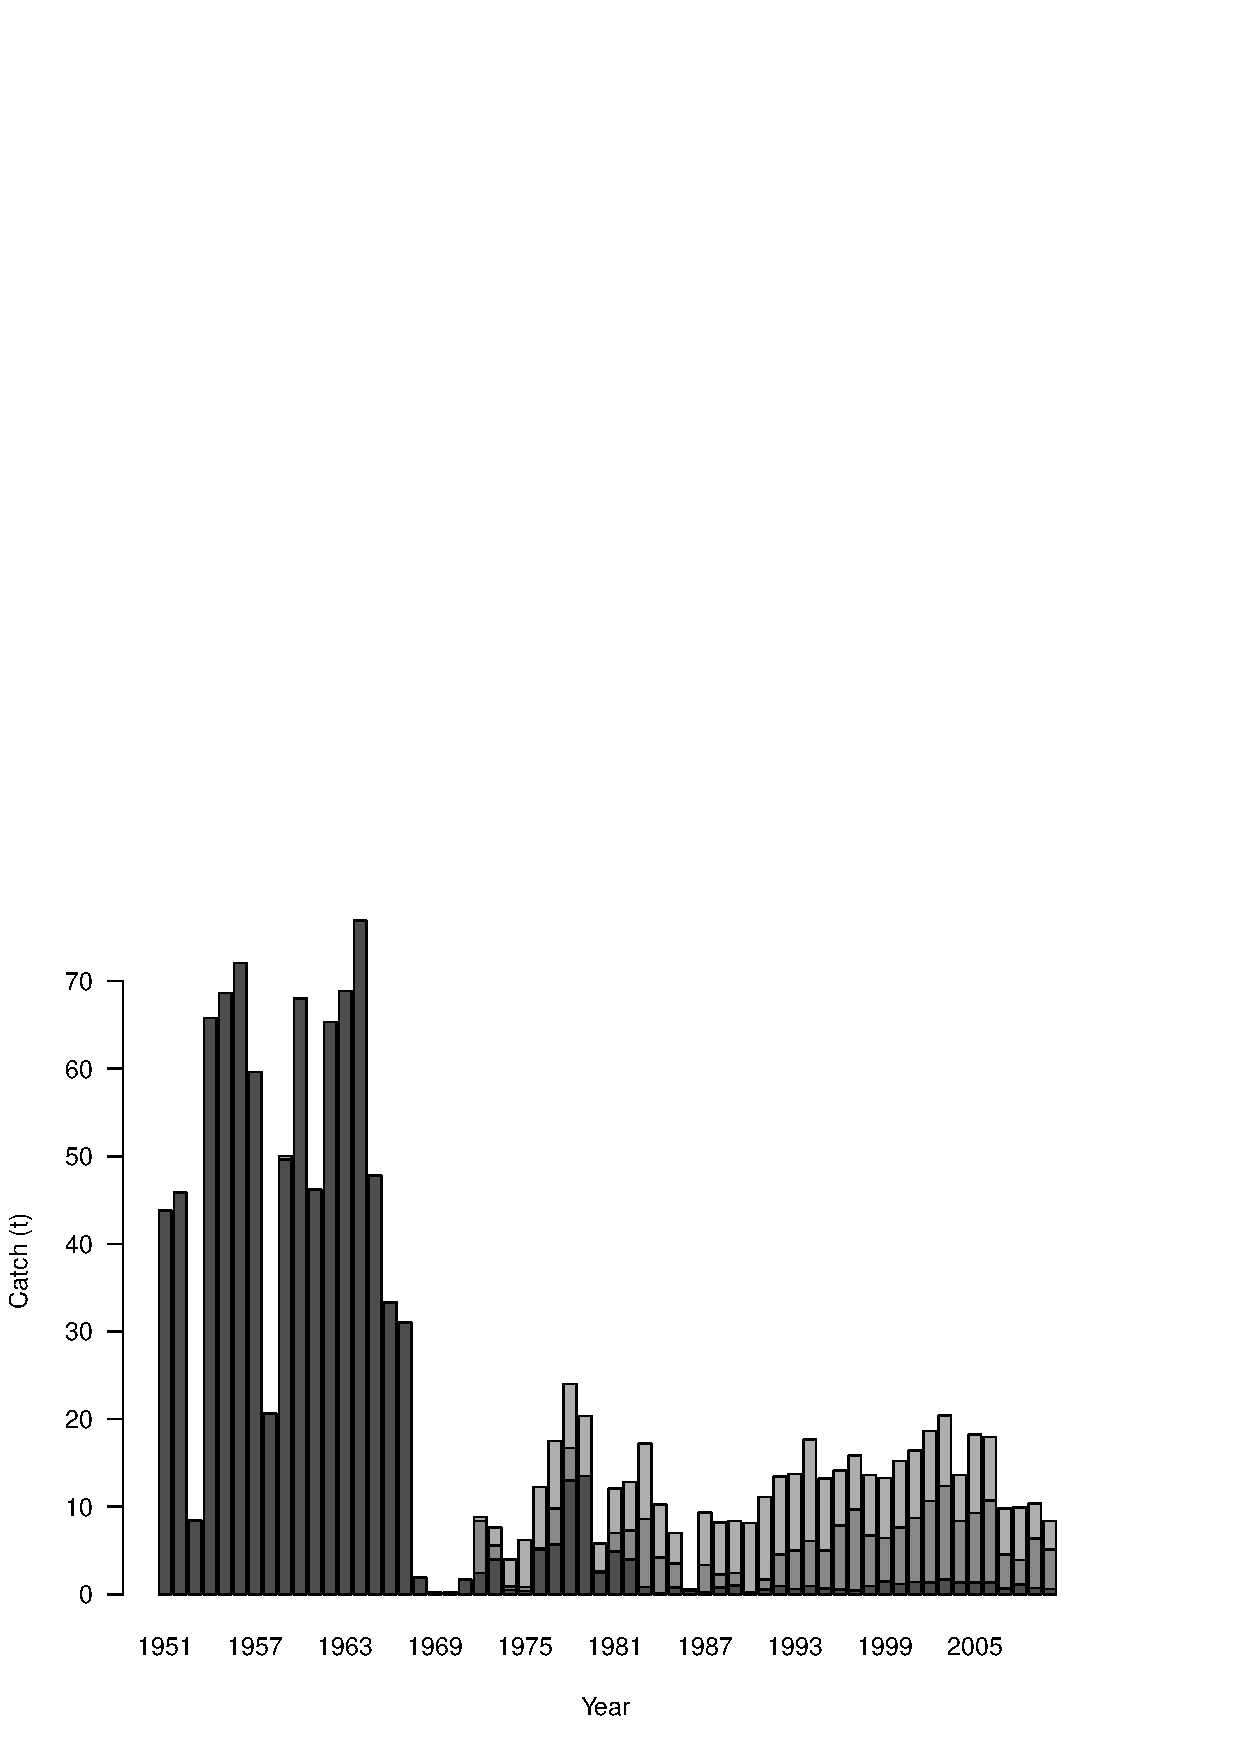
\includegraphics[width=\columnwidth]{iscamfigs/pHerringFig1.pdf}\\
% 	\caption{Total landings of Pacific herring in the Strait of Georgia stock assessment region by purse-seine (dark bars), Sn-roe (medium) and gill net (light bars).}\label{pHerringFig1}
% \end{figurehere}
% 
% 
% \subsection{Data \& control files}
% The available data for the herring fishery consist of commercial landings for each of the three fisheries, age-composition data from each of these fisheries (see Figure \ref{pHerringFig3} for the winter purse seine fishery), average weight-at-age of the catch, and a fisheries independent spawning biomass index (based on spawn deposition).  The spawn survey index is split into two separate series that correspond to a change in methods for estimating spawning deposition between 1987 and 1988.  The model is fit to all of these data and uses the empirical weight-at-age data to convert numbers-at-age to biomass.
% 
% 
% 
% 
% In this example, the command line option \texttt{-sim 000} is invoked to simulate fake data based on parameter values specified in the control file.  Recall the command line option \texttt{-sim} is used to tell \iscam\ to overwrite the existing observations in memory with simulated values (in this case with zero error because the random number seed is set to 000), and then attempt to estimate these model parameters.  If all is working correctly, the \texttt{iscam.par} file should have nearly identical estimates for the model parameters as the initial values that are specified in the control file.
% 
% The control file used in this example is shown here, and there are a couple of things that should be highlighted with simulating data with no error.  First off, the phase for the variance and variance partitioning parameters ($\vartheta$ and $\rho$, respectively) should be set to a negative value and not be estimated.  Second ensure that the upper bound for $\vartheta$ (vartheta or the total precision) is set to a very high value (say 5000) and the initial value is set close to the upper bound (4999 in this case).  The reason for fixing the parameters should be obvious, there is no error in the data to begin and thus its not necessary to estimate the total variance.  The reason to set the initial value of $\vartheta$ to a large value is to minimize the a slight bias due to the lognormal bias correction in the stock-recruitment relationship (i.e., the $-0.5\tau^2$ in \ref{T4.12} or \ref{T4.13}) during the parameter estimation phase.  If you do not specify a large value of $\vartheta$ then it is unlikely that you will obtain nearly exact estimates of the unfished recruitment $R_o$.
% 
% 
% %%Here is a pdf figure rotated.
% \begin{figurehere}
% 	% Requires \usepackage{graphicx}
% 	\centering
% 	%\psfrag{Year}[][c]{Year}
% 	\includegraphics[height=\columnwidth,angle=-90]{iscamfigs/pHerringFig3.pdf}\\
% 	\caption{Age comps for the purse seine fishery in the Strait of Georgia between 1951 and 2010.}\label{pHerringFig3}
% \end{figurehere}
% \vspace{0.1in}
% 
% \noindent \hrulefill\\
% \small
% Control file for the SOG herring example
% \tiny
% \begin{alltt}
% \input{../../../Examples/sogHerring/SOGHerring2010sim.ctl}
% \end{alltt}
% \hrulefill
% \normalsize
% 
% 
% \subsection{Results}
% The ability of the model to estimate the parameters is demonstrated by the estimates of spawning stock biomass and the estimated fishing mortality rates for each of the fisheries.  Shown in Figure \ref{pHerringFig2} is the estimated pre-fishery biomass and the spawning stock biomass for the simulated data where the true values for the spawning stock biomass are shown by the filled circles.  Estimates of spawning stock biomass exactly match the true values that were used to simulate the data.  Departures from the true values when there is no simulated error would imply a structural problem, or potential coding error, and should be investigated further before proceeding with an actual assessment.
% 
% 
% \begin{figurehere}
% 	% Requires \usepackage{graphicx}
% 	\psfrag{Year}[][c]{Year}
% 	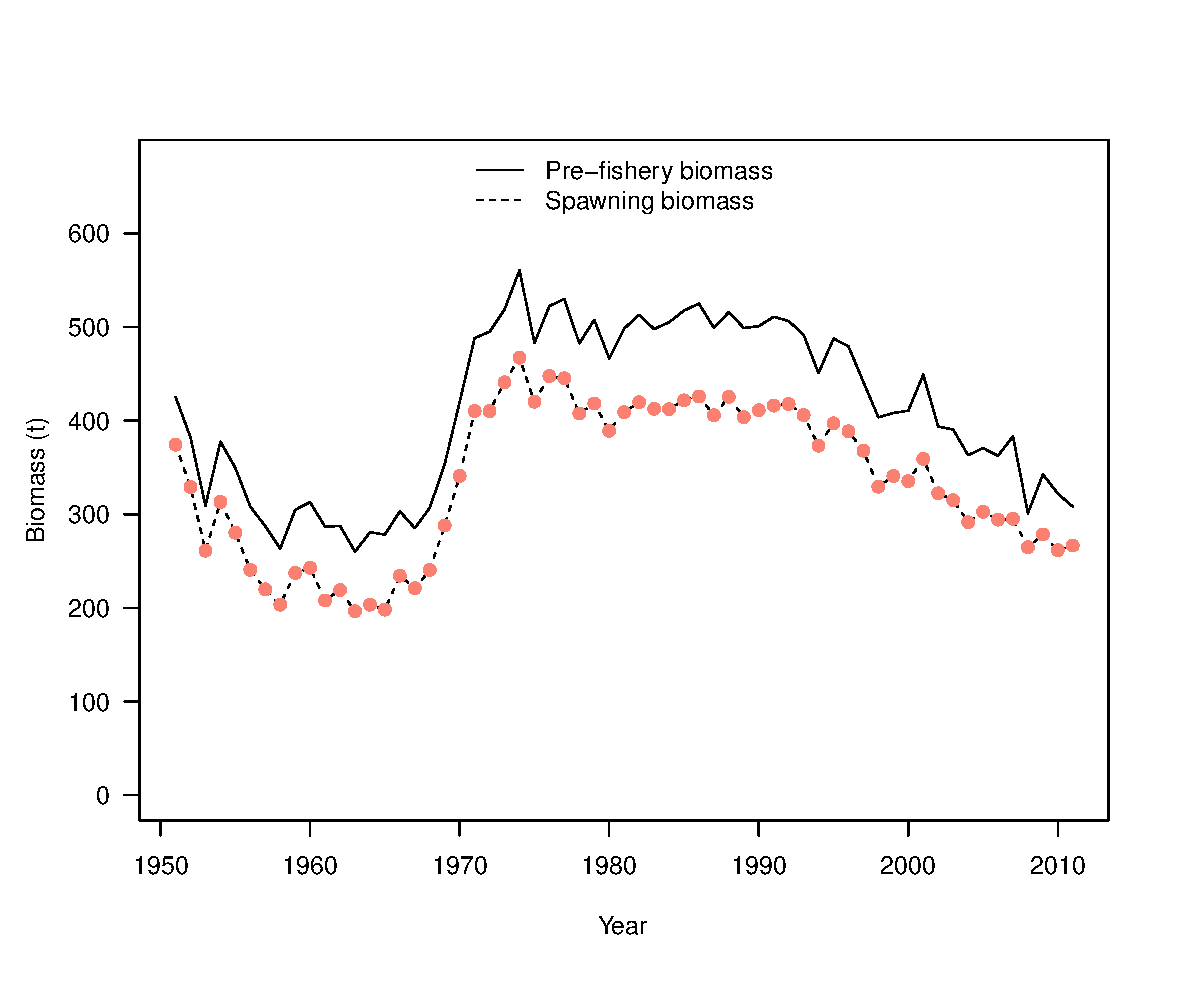
\includegraphics[width=\columnwidth]{iscamfigs/pHerringFig2.eps}\\
% 	\caption{Estimates of pre-fishery biomass and spawning stock biomass (lines) from \iscam\  in comparison to the true spawning stock biomass (filled points) based on the simulation model. No errors were generated in the simulation model.}\label{pHerringFig2}
% \end{figurehere}
% 
% 
% 
% \end{multicols}
% 




%%%%%%%%%%%%%%%%%%%%%%%%%%%%%%%%%%%%%%%%%%%%%%%%%%%%
%%%%%%%%%%%%%%%%%%%%%%%%%%%%%%%%%%%%%%%%%%%%%%%%%%%%
%%%%%%%%%%%%%%%%%%%%%%%%%%%%%%%%%%%%%%%%%%%%%%%%%%%%


\section{Example Assessment: the Namibian hake case study}
\begin{multicols}{2}
As a simple example of fitting \iscam\ to CPUE data only, we use the Namibian hake case study from chapter 10 in the Ecological Detective \citep{hilborn1997ecological}.  In this example the available data consist of catch (thousands of tons) and CPUE (tons per standardized trawl hour).  \cite{hilborn1997ecological} provide three alternative models to the data that range from simple 4 parameter Schaefer production models (observation \& process error only) and a 5 parameter lagged recruitment, growth/survival model.  In this example they assume the stock is at an unfished state in 1967.

To conduct the assessment using \iscam\ with the same unfished assumption in 1965, the 			``Assume unfished in first year (0=FALSE, 1=TRUE)'' flag must be set to 1 (see the following control file). \iscam\ is an age-structured model, and in this example there are no available age-composition data to compare with. Therefore we must also assume a selectivity curve for this fishery.  In this example, selectivity was assume to follow a logistic function with the 50\% vulnerability-at-age equal to 3.5 years with a standard deviation of  1.0 years.  It is also necessary in this case to turn off the estimation of the selectivity parameters by setting the estimation phase to a negative number (e.g., -1).  

For the estimated leading parameters, two of the six parameters are not estimated \verb"#log_m" and \verb"#rho", which is the instantaneous natural mortality rate and the proportion of the total error that is associated with observation errors.  A bounded uniform prior is assumed for $R_o$ and a beta prior for steepness $h$ with an expected value of 0.6.  The natural mortality rate $M$ is assumed known and fixed at a value of 0.345.  A uniform bounded prior is assumed for the log of the average recruitment level, and a non-informative gamma prior is assumed for the total precision $\kappa$.  In this example we assume that the total error is allocated to observation and process error equally ($\rho= 0.5$).

\tiny
\noindent \hrulefill
\begin{alltt}
Control file for the Namibian hake data.
\input{../../../examples/ECODETECTIVE/Data/NamibianHake.ctl}
\end{alltt}
\hrulefill
\normalsize

To convert numbers-at-age to biomass, growth was based on the von Bertalanffy growth parameters in the \verb"NamibianHake.dat" file and the allometric relationship $w_a=a(l_a)^b$. Maturity-at-age is  based on the logistic function with age-4 being the age at 50\% maturity and 0.2 is the standard deviation. The plus group age was assumed to be 25 years, and there is only one fishing gear exploiting this stock.

Catch is taken by a single gear each year between 1965 and 1987, and the relative abundance index is based on the catch per standardized hour of trawling for the commercial gear.  It is assumed that each CPUE observation is assumed to have the same error distribution, and the relative weights of each observations are all set equal to one.

There is no age-composition data to speak of, but \verb"#na_gears" must have a value of 1 in order to proceed with reading the remaining portion of the data file.

\tiny
\noindent \hrulefill
\begin{alltt}
Data file for the Namibian hake data.
\input{../../../examples/ECODETECTIVE/DATA/NamibianHake.dat}
\end{alltt}
\hrulefill
\normalsize

%%Results for Namibian hake.
\subsection{Maximum likelihood estimates of the model parameters}
Estimates of unfished spawning biomass is 2,877, steepness is 0.79, MSY is 266, and \fmsy is 0.33.  These results are  very similar to those obtained by \cite{hilborn1997ecological} for the Schaefer model with observation error.  Estimates of the total standard deviation amount to 0.16 which equally breaks down to 0.081 for observation and process errors.

\begin{figurehere}
	\centering
	\includegraphics[width=0.9\columnwidth]{iscamFigs/NhakeFigs.eps}
	\caption{Estimates of total biomass and spawning biomass, observed and predicted CPUE, for the Namibian hake data from \iscam. Unfished biomass, \bmsy, and MSY based depletion levels are shown as horizontal dotted lines.}\label{fig4}
\end{figurehere}

\subsection{Bayesian analysis of model parameters \& policy parameters}
Marginal posterior distributions of model parameters were constructed by using the metropolis algorithm built into ADMB to sample from the joint posterior distribution.  This is accomplished by running \iscam\ in -mcmc mode followed by the -mceval option to produce the \verb"iscam.mcmc" output file.  In this example an MCMC chain of length 1,000,000 was run and samples were taken systematically every 500 iterations (\verb"-mcsave 500"), which results in a posterior sample size of 2000.

Uniform prior distributions for the unfished recruitment and average recruitment ($R_0$ and $\bar{R}$), and non-informative gamma prior for the precision parameter ($1/\vartheta$).  In the case of the steepness parameter, a non-informative beta prior was used ($p(h)\sim beta[1.01,1.01]$), where steepness is re-scaled to the interval 0.2-1.0 (i.e, $(h-0.2)/0.8$) such that a 0 probability was assigned for $h$ values less than 0.2.  In comparison to the results obtained by \cite{hilborn1997ecological} using a biomass production model with lagged recruitment and a Beverton-Holt recruitment function, the data here appear to have some information about the steepness parameter (Fig. \ref{fig5}).  This owes in part to differences in assumptions about growth, maturity and selectivity between the LRGS model used by \cite{hilborn1997ecological} and this \iscam\ example.

\begin{figurehere}
	% Requires \usepackage{graphicx}
	\centering
	% \psfrag{log.ro}[c][][0.75]{$\ln(R_0)$}
	% 	\psfrag{log.rbar}[c][][0.75]{$\ln(\bar{R})$}
	% 	\psfrag{kappa}[c][][0.75]{$\vartheta$}
	% 	\psfrag{h}[c][][0.75]{$h$}
	%%\includegraphics[width=\columnwidth]{iscamFigs/fig5.eps}\\
	\includegraphics[width=0.9\columnwidth]{iscamFigs/nHakeparameters.pdf}\\
	\caption{Marginal posterior probability densities (histograms) and prior densities (lines) for unfished recruitment $R_0$, steepness $h$, mean recruitment $\bar{R}$ and recruitment compensation $\kappa$ for the Namibian hake case study.}\label{fig5}
\end{figurehere}

Marginal posterior densities can also be produced for derived quantities such as MSY based reference points (Fig \ref{fig6}).   Again, although not directly comparable due to structural differences between \iscam\ and the LRGS model, the marginal posterior distributions for MSY and $B_0$ are very similar.  More importantly however is that these marginal distributions can also be used to calculate the probability that the stock is currently overfished and if overfishing is occurring.  This is normally represented from a maximum likelihood perspective where the trends in biomass relative to \bmsy and fishing mortality rates relative to \fmsy are plotted against each other (these are known as KOBE plots, Fig \ref{fig7}).

\begin{figurehere}
	% Requires \usepackage{graphicx}
	\centering
	% \psfrag{bo}[c][][0.75]{$B_0$}
	% 	\psfrag{bmsy}[c][][0.75]{\bmsy}
	% 	\psfrag{msy}[c][][0.75]{MSY}
	% 	\psfrag{fmsy}[c][][0.75]{\fmsy}
	%%\includegraphics[width=\columnwidth]{iscamFigs/fig6.eps}\\
	\includegraphics[width=0.9\columnwidth]{iscamFigs/nHakerefpoints.pdf}\\
	\caption{Marginal posterior probability densities for unfished spawning biomass $B_0$, optimal spawning biomass \bmsy, MSY and \fmsy\ for the Namibian hake case study.}\label{fig6}
\end{figurehere}

To represent changes in stock status over time, the default plot compares estimates of spawning stock biomass relative to the estimates of \bmsy versus fishing mortality rates relative to \fmsy.  Uncertainty in stock status for the last year is based on the joint posterior distribution and a credible interval is given by a contour plot that represents a `fried egg'.

\begin{figurehere}
	\centering
	% \psfrag{bstatus}[c][][0.75]{$B_t/$\bmsy}
	% 	\psfrag{fstatus}[c][][0.75]{$F_t/$\fmsy}
	%%\includegraphics[width=\columnwidth]{iscamFigs/fig7.eps}\\
	\includegraphics[width=0.9\columnwidth]{iscamFigs/NhakeKobeplot.pdf}\\
	\caption{Stock status plot (or Kobe plot) where the ``fried egg'' represents uncertainty.}\label{fig7}
\end{figurehere}

\end{multicols}



%%%%%%%%%%%%%%%%%%%%%%%%%%%%%%%%%%%%%%%%%%%%%%%%%%%%
%%%%%%%%%%%%%%%%%%%%%%%%%%%%%%%%%%%%%%%%%%%%%%%%%%%%
%%%%%%%%%%%%%%%%%%%%%%%%%%%%%%%%%%%%%%%%%%%%%%%%%%%%
\section{Example Assessment: the Pacific hake fishery}
\begin{multicols}{2}
\subsection{Data \& assumptions}
As more complex example assessment, the data from the Pacific hake fishery is used.  Pacific hake (\textit{Merluccius productus})  in the Northeast Pacific has a migratory coastal stock that is harvested by US and Canadian fishing fleets during the summer and late fall.  This data is an extension to the previous work in \cite{Martell2008pam}.  In this example the data has been restricted to the years 1977-2009, as this was a period when catch-age data from both the Canadian and US fisheries was available and could be aggregated using a weighted average based on the catch proportion from each nation.

The data from this fishery consists of a combined total catch, a relative abundance index from an acoustic survey conducted on a triannual and biannual basis, age-composition data from the commercial fishery, and finally age-composition data from the acoustic trawl survey. The coastal Pacific hake stock undergo an annual migration from spawning grounds in the south near Baja California Sur in the winter to summer feeding grounds to the north; the extent of the northward migration is highly variable and ranges from Oregon--Washington to Southeast Alaska in some years.  Larger/older fish tend to migrate further north.  Inter-annual variation in the extent of the migration leads to variation in selectivity to the fishery.  To accommodate the time-varying selectivity, a total of 85 nodes for a bicubic spline are estimated (17 nodes for the year effect, and 5 nodes for the age effect, see Fig. \ref{Fig3}).

\begin{figurehere}
	\centering
	\includegraphics[width=0.8\columnwidth]{iscamFigs/phakefig15.eps}\\
	\caption{Combined observed landing from the US and CAN fisheries for Pacific hake between 1977 and 2009.}\label{fig8}
\end{figurehere}

In this example it was assumed that recruitment follows a Beverton-Holt relationship, the stock is not at its unfished state in 1977, natural mortality is independent of age and constant over time, and survey selectivity is asymptotic and time-invariant.  


Here is the \iscam\ control file for the Pacific hake data, and the data file is provided at the end of this section on page \pageref{HakeDataFile}.  The observed combined landings from both the US and Canadian zones have averaged about 233,000 metric tons between 1977 and 2009, and in the last 10 years has averaged 270,000 mt with a peak in 1994 of 361,000 mt  (Fig. \ref{fig8}.)\\
\tiny
\noindent \hrulefill
\begin{alltt}
\input{../../../examples/PacificHake/Data/2010/PHake2010.ctl}
\end{alltt}
\hrulefill
\normalsize


%
%\begin{figurehere}
%	\centering
%	\includegraphics[width=0.4\columnwidth]{iscamFigs/phakefig1.eps}\\
%	\caption{Assumed age-schedule information for this example assessment.}\label{fig8b}
%\end{figurehere}


\subsection{Maximum likelihood estimates}
A total of 176 model parameters were estimated and it took  roughly 10 seconds to obtain maximum likelihood estimates, including the calculations for the Hessian matrix on a MacBook Pro, with a 2.66 GHz Intel Core i7 processor.

Maximum likelihood estimates of total biomass and spawning biomass along with estimates of $B_0$ and \bmsy are shown in Fig. \ref{fig9}.  Starting in 1977, estimates of spawning biomass was just slightly less than the estimate of \bmsy.  Starting in the 1980's, spawning biomass increased to a maximum in 1990 owing to two very large year classes (1980 and 1984, Fig. \ref{fig10}). Between 1985 and 1999, recruitment ranged between average and median values and the spawning stock biomass declined to less than \bmsy values in 2001 while fisheries removals exceeded 200,000 mt per year.  Another significant year class (1999) was responsible for rebuilding the spawning stock biomass up to 2004, and since 2005, the spawning stock biomass has continued to decline.

Information to estimate age-1 recruitment for Pacific hake comes from the catch-age composition data.  Between 1978 and 2009 the average age-1 recruitment is estimated to be 2.72 billion individuals and the median value is 1.16 billion individuals (Fig. \ref{fig11}).  The maximum likelihood estimate of the standard deviation in recruitment ($\tau$, see eq. \ref{T4.2} on page \pageref{tab:statistical_catch_age_model}) was 1.29 given the prior information specified in the control file for this assessment.


\begin{figurehere}
	\centering
	\includegraphics[width=0.9\columnwidth]{iscamFigs/phakefig2.eps}\\
	\caption{Maximum likelihood estimates of total biomass and spawning stock biomass for Pacific hake along with reference points (dotted lines) for unfished spawning biomass $B_0$ and \bmsy.}\label{fig9}
\end{figurehere}


\begin{figurehere}
	\centering
	\includegraphics[width=0.9\columnwidth]{iscamFigs/phakefig14.eps}\\
	\caption{Maximum likelihood estimates of age-1 recruits from 1978 to 2009, with median and average values shown as the horizontal dashed and dotted lines.}\label{fig10}
\end{figurehere}

Current estimates of stock status relative to \bmsy\ and the removal rate relative to \fmsy is estimated to be in the critical zone in term of the Department of Fisheries and Oceans Canada, Fisheries Management Framework (Fig. \ref{fig11}).  Estimates of the spawning stock biomass are less than 80\% of \bmsy and are currently in the cautious zone.  Estimates of fishing mortality rate are roughly 1.5 times the estimate of \fmsy.  Maximum likelihood estimates of \bmsy and \fmsy are 1.13 million mt 0.336, respectively. 

\begin{figurehere}
	\centering
	\includegraphics[width=0.9\columnwidth]{iscamFigs/phakefig8.eps}\\
	\caption{Maximum likelihood estimates of stock status ($B_t/$\bmsy) and removal rate ($F_t/$\fmsy) for Pacific hake relative to the Department of Fisheries and Oceans Canada's  Fisheries Management Framework.}\label{fig11}
\end{figurehere}

Model fit can be partially judged by the residual patterns between the observed and predicted data (Fig. \ref{fig12}).  The catch data are assumed to be measured fairly accurately with a small standard deviation ($\sigma_C=0.025$) in measurement errors; the largest residual in the catch is just less than 100 mt in 1981.  

Recall that \iscam\ directly estimates annual recruitment values, and the reported residuals in Fig. \ref{fig12} correspond to the log differences between the estimated recruitment and a Beverton-Holt model prediction where $R_0$ and steepness $h$ are the estimated parameters for the stock recruitment model.  The strong 1980, 1984 and 1999 cohorts, show up as strong positive residuals in 1981, 1985 and 2000 in the residual plot (note that the age-at-recruitment is 1 year).  The 2002 and 2004 cohorts appear to be well below the median values in recent years, and the 2005 cohort is currently estimated to be the next largest cohort since 1999.

\begin{figurehere}
	\centering
	\includegraphics[width=0.9\columnwidth]{iscamFigs/phakefig11.eps}\\
	\caption{Residuals between the observed and predicted catch, deviations between estimated recruitment and a deterministic Beverton-Holt model, and the observed and predicted relative abundance data from the acoustic survey.}\label{fig12}
\end{figurehere}


\subsection{Time-varying selectivity}
Estimates of time-varying selectivity for the commercial fishery were based on estimating 85 nodes (17 years and 5 ages) and interpolating between these nodes using a bicubic spline.  The estimated nodes in \iscam\ are equidistant, and the total number of estimated nodes is specified in the control file.  Increasing the number of estimated nodes should improve the overall fit to the age-composition data; however, this comes at the expense of increasing the associated uncertainty in overall model parameter estimates.  To ensure that the model is not over-fitting the data, there are two additional penalties that are added to the objective function that limit the rate of change in age-effects (penalty weight for second differences), and how much dome-shaped is allowed in the age-effects.  Increasing the penalty weight on second differences insures a smoothed increase or decrease in the selectivity-at-age, and increasing the weight on the dome-shaped penalty reduces the amount of dome-shaped selectivity that can occur.  Again, these penalty weights are specified in the control file  in the selectivity parameters section.

In the Pacific hake example, estimates of selectivity increase with age during the late 1970s and early 1980s (Fig. \ref{fig13}).  As the 1980 and 1984 cohorts recruit to the fishery, the selectivity shifts to younger ages, and becomes more dome-shaped.  At the peak of the spawning stock biomass in 1990, selectivity increases continuously with age, and is more or less asymptotic until the 1999 cohort enters the fishery.  Recent estimates of selectivity indicate that the 1999 cohort (age-10 in the year 2009) is still strongly selected for, but as the biomass of the 1999 cohort erodes there is an apparent increase in selectivity for older ages (Fig. \ref{fig13}).

\begin{figurehere}
	\centering
	\includegraphics[width=0.9\columnwidth]{iscamFigs/phakefig9a.eps}\\
	\caption{Estimates of selectivity for the commercial fishery.}\label{fig13}
\end{figurehere}


\begin{figurehere}
	\centering
	\includegraphics[width=0.9\columnwidth]{iscamFigs/phakefig13a.eps}\\
	\caption{Observed age-composition (top panel) and Pearson residuals between observed and predicted proportions-at-age in the commercial fishery (bottom panel, with negative residuals given by dark circles).}\label{fig13a}
\end{figurehere}

The residual patterns in the age composition data from the commercial fishery don't appear to have any significant pattern that would indicate a major model mis-specification (Fig. \ref{fig13a}).  There is a tendency for age-2 proportions to have more negative residuals and age-3 positive residuals, but over all these residuals are fairly small.  This is not much of a surprise given the flexibility of the time-varying selectivity that was assumed in the commercial fishery.


Although not shown here, the residual pattern for the survey age composition also appears to be random, and in this case a time-invariant asymptotic selectivity curve was used for the acoustic survey. Survey data from 1995 to 2007 were assumed to be twice as accurate in comparison to the data collected prior to 1995 when spatial coverage of the survey was incomplete.  Also, the 2009 survey carries no weight as this survey was contaminated by the presence of Humboldt squid (\textit{Dosidicus gigas}) during the 2009 survey.  Additional details about the data for the Pacific hake assessment and the methods used to aggregate the age-composition for the US and CAN fisheries can be found in \cite{Martell2009}.

\subsection{Bayesian implementation}
To obtain samples from the joint posterior distribution and obtain median values and credible intervals, \iscam\ was run using the Metropolis-Hastings routine that is built into ADMB.  In this example, 2000 systematic samples from a chain of length 1,000,000 was used.  The total runtime for conducting a MCMC sample  of length 1,000,000 was 39 minutes and 56 seconds with 176 estimated parameters.

The marginal posterior distributions and the corresponding prior distributions are shown in Fig. \ref{fig14}.  There is no information in the data about the underlying steepness of the stock recruitment relationship; this is clearly shown by the marginal posterior distribution for $h$ reflects the assumed (\emph{ad hoc}) prior distribution.

\begin{figurehere}
	\centering
	% \psfrag{log.ro}[c][][0.5]{$\ln(R_0)$}
	% \psfrag{log.rbar}[c][][0.5]{$\ln(\bar{R})$}
	% \psfrag{h}[c][][0.5]{$h$}
	% \psfrag{rho}[c][][0.5]{$\rho$}
	% \psfrag{log.m}[c][][0.5]{$\ln(M)$}
	% \psfrag{kappa}[c][][0.5]{$\vartheta$}
	\includegraphics[width=0.9\columnwidth]{iscamFigs/phakefig5.eps}\\
	\caption{Marginal posterior densities and prior densities for the leading parameters in \iscam.}\label{fig14}
\end{figurehere}

The prior distributions for each of the estimated leading parameters are specified in the control file.  In this example, a normal prior was assumed for the unfished recruitment ($\ln(R_0)$) and the log of the natural mortality rate ($\ln(M)$), a beta prior for the steepness ($h$) and the fraction of the total error that is associated with observation error ($\rho$), and a non-informative gamma prior for the total precision ($\vartheta$).  A uniform prior was specified for the average recruitment ($\ln(\bar{R})$).

Recent trends in the spawning stock biomass, and depletion, along with the associated uncertainty in the form of a credible interval are given in Table \ref{iscam.T1}.  Projected estimates of spawning stock depletion at the start of 2010 is 22\%, with a lower bound of 7.5\% and an upper bound of 53.2\%.  This translates into a projected spawning stock biomass of 670,000 mt with a 95\% credible interval of 255,000 mt to 1,506,000 mt.

\begin{tiny}
% latex.default(tail(t1, 10), file = filename, rowname = NULL,      caption = cap, cgroup = cgrp, n.cgroup = ncgrp, label = "iscam.T1") 
%
\begin{tablehere}
 \caption{Median estimate and 5\% and 95\% credible 
					intervals for spawning stock biomass, and spawning 
					stock depletion. These estimates are based on sampling the
						joint posterior distribution using MCMC.\label{iscam.T1}} 
 \begin{center}
 \begin{tabular}{rcrrrcrrr}\hline\hline
\multicolumn{1}{c}{\bfseries  }&
\multicolumn{1}{c}{\bfseries }&
\multicolumn{3}{c}{\bfseries Spawning stock biomass}&
\multicolumn{1}{c}{\bfseries }&
\multicolumn{3}{c}{\bfseries Depletion}
\tabularnewline \cline{1-9}
\multicolumn{1}{c}{Year}&\multicolumn{1}{c}{}&\multicolumn{1}{c}{5\%}&\multicolumn{1}{c}{median}&\multicolumn{1}{c}{95\%}&\multicolumn{1}{c}{}&\multicolumn{1}{c}{5\%}&\multicolumn{1}{c}{median}&\multicolumn{1}{c}{95\%}\tabularnewline
\hline
$2001$&&$0.884$&$0.997$&$1.130$&&$0.202$&$0.336$&$0.524$\tabularnewline
$2002$&&$1.047$&$1.194$&$1.384$&&$0.240$&$0.403$&$0.635$\tabularnewline
$2003$&&$1.913$&$2.150$&$2.549$&&$0.434$&$0.727$&$1.142$\tabularnewline
$2004$&&$2.075$&$2.340$&$2.815$&&$0.474$&$0.795$&$1.244$\tabularnewline
$2005$&&$1.742$&$1.994$&$2.452$&&$0.404$&$0.679$&$1.063$\tabularnewline
$2006$&&$1.293$&$1.524$&$1.961$&&$0.308$&$0.521$&$0.820$\tabularnewline
$2007$&&$0.904$&$1.139$&$1.577$&&$0.224$&$0.389$&$0.632$\tabularnewline
$2008$&&$0.602$&$0.848$&$1.315$&&$0.158$&$0.288$&$0.503$\tabularnewline
$2009$&&$0.378$&$0.729$&$1.406$&&$0.108$&$0.242$&$0.497$\tabularnewline
$2010$&&$0.255$&$0.670$&$1.506$&&$0.075$&$0.222$&$0.532$\tabularnewline
\hline
\end{tabular}

\end{center}

\end{tablehere}


\end{tiny}

Relative to the spawning stock depletion reference points, the median estimate of spawning stock biomass falls in the critical zone (Fig. \ref{fig16}).  Estimates of spawn stock depletion is very uncertain; there is a fairly high probability that the stock is also in the critical zone, or less than 40\% of \bmsy.

\begin{figurehere}
	\centering
	\includegraphics[width=0.9\columnwidth]{iscamFigs/phakefig12.eps}\\
	\caption{Median estimates of spawning stock depletion and 95\% credible interval based 2000 samples from the joint posterior distribution. Transition between the critical, cautious and healthy zones is defined as 0.4\bmsy/$B_0$ and 0.8\bmsy/$B_0$, respectively }\label{fig16}
\end{figurehere}

\begin{scriptsize}
% latex.default(t1, "", file = filename, caption = cap, label = "iscam.T2") 
%
\begin{tablehere}
 \caption{Maximum likelihood estimates (MLE) and standard deviations (SD)
				based on the inverse Hessian for the six leading parameters. Median
				values and the 95\% credible interval based on posterior samples.\label{iscam.T2}} 
 \begin{center}
 \begin{tabular}{lrrrrr}\hline\hline
\multicolumn{1}{l}{}&\multicolumn{1}{c}{MLE}&\multicolumn{1}{c}{SD}&\multicolumn{1}{c}{Median}&\multicolumn{1}{c}{2.5\%}&\multicolumn{1}{c}{97.5\%}\tabularnewline
\hline
$\ln(R_0)$&$ 1.167$&$0.326$&$ 1.238$&$ 0.674$&$ 1.958$\tabularnewline
$h$&$ 0.688$&$0.214$&$ 0.669$&$ 0.370$&$ 0.932$\tabularnewline
$\ln(M)$&$-1.478$&$0.049$&$-1.457$&$-1.554$&$-1.363$\tabularnewline
$\ln(\bar{R})$&$-0.168$&$0.119$&$-0.103$&$-0.343$&$ 0.177$\tabularnewline
$\rho$&$ 0.293$&$0.043$&$ 0.305$&$ 0.227$&$ 0.405$\tabularnewline
$\vartheta$&$ 0.525$&$0.053$&$ 0.517$&$ 0.422$&$ 0.623$\tabularnewline
\hline
\end{tabular}

\end{center}

\end{tablehere}


\end{scriptsize}

\end{multicols}




Here is the data file for \iscam.
\tiny
\begin{alltt}
  \input{../../../examples/PacificHake/DATA/2010/PHake2010.dat}\label{HakeDataFile}
\end{alltt}
\normalsize




%    %!TEX root = /Users/stevenmartell/Documents/CURRENT PROJECTS/iSCAM-trunk/fba/BC-herring-2011/WRITEUP/BCHerring2011.tex
\section{Methods}
	\subsection{Input data \& assumptions}
	\subsubsection{Catch data}
	For each of the statistical areas, the required input data for \iscam\ consists of a catch time series for each of the fishing fleets.  For the BC herring fishery, the annual total removals has been partitioned into three distinct fishing fleets (or fishing periods, see Figure \ref{FigCatch}).  The first fleet is a winter seine fishery that has been in operation since the start of the assessment in 1951, the second is a seine-roe fishery that commenced in 1972 in the Strait of Georgia, and the third fleet is a gillnet fishery that targets females on the spawning grounds. The model is fit to the catch time series information and assumes measurement errors are lognormal, independent and identically distributed.  The assumed standard deviation in the catch observation data must be specified in the control file and it is assumed that measurement errors in the catch is the same for all fishing periods.  The units of the catch are given in 1000s of metric tons.
	
	In addition to the commercial catch, removals from fisheries independent surveys must also be specified in \iscam. Two additional fleets are specified to represent the spawn survey, where the spawn survey is broken into two distinct time periods pre-1988 and post-1988, the year when the survey switched from surface surveys to dive surveys.  This partitioning of the data is done for two reasons: (1) to allow for different catchability coefficients to be specified for the early and late periods, and to allow for more weight to be placed on the contemporary data due to improved precision in the estimates of egg layers. 

%TODO decide if the test fishery data is going to be looked at here or in the appendix
	% In the case where the test fishery data has been separated from the seine roe fishery, an additional fleet is specified in the data file and fishing mortality rates for the test fishery are also estimated in years when the catch is greater than 0.
	
\begin{figure}[!tbp]
	% Requires \usepackage{graphicx}
	\includegraphics[width=\textwidth]{../Figs/iscam_fig_CatchMajorAreas.pdf}\\
	\caption{Historical catch of herring in the five major stock areas between 1951 and 2011 for the winter purse seine fishery (dark bars), seine-roe fishery (grey bars), and gillnet fishery (light grey bars). Units of catch are in thousands of metric tons.}\label{FigCatch}
\end{figure}
	
	\subsubsection{Relative abundance data}
Herring spawn surveys have been conducted throughout the B.C. coast beginning in the 1930s. Prior to 1988, spawn surveys were conducted from the surface either by walking the beach at low tide or using a drag from a skiff to estimate the shoreline length and width of spawn. Egg layers were sampled visually and are used to calculate egg densities following the methods of \cite{schweigert2001stock}. Beginning in 1988, herring spawn surveys using SCUBA methods were introduced and were implemented coastwide within a couple of years initially being conducted by DFO staff and eventually through contract divers hired through the test fishing program. Prior to the 2006 Larocque ruling, the test fishing program was funded through an allocation of fish by industry. In years since the 2006 Larocque ruling, the availability of resources to conduct dive surveys in all areas has been reduced. For 2011, dive surveys were conducted in all major and minor assessment regions, with the exception of Area 2W where snorkelling and surface survey methods were also used. As in earlier years, a few minor spawning beds outside the main assessment areas were surveyed by SCUBA or surface methods where resources permitted.


The locations of the spawning beds for the five major and two minor stock areas are shown in Figure \ref{figSpawnMaps}.  Egg density estimates are used to calculate a fishery-independent index of herring spawning biomass, referred to as the spawn survey index hereafter \citep{schweigert2001stock}.

\begin{figure}[!tbp]
	% Requires \usepackage{graphicx}
	\centering
	\includegraphics[scale=0.35]{../Figs/PBSfigs/2011_spawn_HG_2E_July13.pdf}
	\includegraphics[scale=0.35]{../Figs/PBSfigs/2011_spawn_HG_2W_July13.pdf}\\
	\includegraphics[scale=0.35]{../Figs/PBSfigs/2011_spawn_PRD_July13.pdf}
	\caption{Preliminary Spawning activity for Haida Gwaii (top panels) and Prince Rupert District (bottom) in 2011.}
\end{figure}
\begin{figure}[!tbp]
	% Requires \usepackage{graphicx}
	\ContinuedFloat
	\centering
	\includegraphics[scale=0.35]{../Figs/PBSfigs/2011_spawn_CCJuly13.pdf}
	%\includegraphics[scale=0.5]{../Figs/PBSfigs/2011-SOG-Prelim-WG.pdf}
	\includegraphics[scale=0.35]{../Figs/PBSfigs/2011_spawn_SOG_July13.pdf}\\
	\includegraphics[scale=0.35]{../Figs/PBSfigs/2011_spawn_WCVI_August16.pdf}
	\caption{Preliminary Spawning activity for Central Coast (top left panel), Strait of Georgia (top right) in 2011 and west coast Vancouver Island (bottom).}\label{figSpawnMaps}
\end{figure}
% \begin{figure}[!tbp]
% 	% Requires \usepackage{graphicx}
% 	\ContinuedFloat
% 	\centering
% 	%\includegraphics[scale=0.5]{../Figs/PBSfigs/2011-WCVI-Prelim-WG.pdf}\\
% 	\includegraphics[scale=0.5]{../Figs/PBSfigs/2011_spawn_WCVI_August16.pdf}\\
% 	\caption{Preliminary Spawning activity in 2011 for the West Coast of Vancouver Island (includes minor stock area 27).}\label{figSpawnMaps}
% \end{figure}

	The spawn survey is conducted after the fisheries in the area have been completed; therefore, it is assumed that all the mortality for the year has occurred just prior to commencing the spawning survey. The fisheries independent survey estimates egg density and total spawn area, and from this information the total female spawning biomass can be estimated assuming the 200 eggs per gram of female body weight or 100 eggs per gram of mature body weight of both sexes \citep{hay1985reproductive,hardwick1973biomass}. The assumed selectivity for the spawn survey is fixed to the maturity schedule for herring and the mean weight-at-age data comes from empirical observations based on biological samples.  	
	
\begin{figure}[!tbp]
	% Requires \usepackage{graphicx}
	\includegraphics[width=\textwidth]{../Figs/iscam_fig_SurveyMajorAreas.pdf}\\
	\caption{Spawn survey index for Strait of Georgia between 1951 and 2011. The units are actual estimates of spawning biomass (1000s tons), but only the trend information is used in the model fitting.}\label{FigSurvey}
\end{figure}
	
	\subsubsection{Biological samples}
	
	Biological samples are collected from both commercial catch and from the test fishery program.  Commencing  in 1975, test fishery charters supplemented biological samples in areas where catch sampling that was not representative of the stock in that area (i.e., fishing solely on spawning aggregations), or in closed areas. Prior to 2006, test fishing charters were funded through an allocation of fish to the test program; the program is now fully funded by DFO.  Through a contract with DFO, the Herring Conservation and Research Society (HCRS) sub-contracts a number of vessels to collect biological samples.  Industry also conducts pre-season test sets for roe-quality testing in open areas and supplementary biological samples are provided as part of this program.  The following data are collected for all biological samples: fish length, weight, sex, and maturity.  Subsequently these sources of data are compiled and used as the information on mean weight-at-age and catch-at-age data that are the essential input data for the stock assessment model.
	
	During the 2010/2011 season a total of 248 biological samples were collected, of which 151 were collected from the test fishery, 57 were collected from the roe fishery, 16 from the food \& bait fishery, 4 from Spawn on Kelp (SOK) operations, and 16 from the summer trawl research survey (Table \ref{table:PartII:bioSamples}).  Note that the definition of a sample is roughly 100 individual fish.  A summary of biological samples collected from commercial and pre-fishery charters from 2002/03--2010/11 is presented in Table \ref{table:PartII:sampleSizes} and the spatial locations of the biosamples are presented in Figure \ref{fig:FIGS_2011_biosamples_maps_2011_biosamplesNC_SAR}.

\begin{table}
	\caption{Summary of biological samples collected and processed from all sources from the 2010/11 herring season.}
	\label{table:PartII:bioSamples}
	\begin{center}
		\begin{tabular}{cccccc}
		\hline
		& \multicolumn{3}{c}{Commercial samples} &  \\
		Stock & Roe fishery & SOK fishery & F\&B & Test fishery & Research\\
		\hline
		HG (QCI 2E) &  &  &  & 13\\
		PRD & 29 & 1 &  & 24\\
		CC &  &  &  & 30\\
		SOG & 18 &  & 20 & 60\\
		WCVI &  &  &  & 14 & 16\\
		Area 2W &  &  &  & 10\\
		Area 27 &  & 3\\
		Other Areas\\
		\hline
		Total & 57 & 4 & 16 & 151 & 16\\
		\hline
		\end{tabular}
	\end{center}
\end{table}

\begin{table}
	\caption{Summary of biological samples collected and processed from commercial catch and test fishery charters from 2002/03-2010/11.}
	\label{table:PartII:sampleSizes}
	\begin{center}
\begin{tabular}{cccc}
\hline
Fishing season & Commercial fishery samples & Charter and research samples & Total\\
\hline
2002/03 & 120 & 287 & 407\\
2003/04 & 79 & 222 & 301\\
2004/052 & 83 & 191 & 274\\
2005/06 & 46 & 164 & 210\\
2006/07 & 114 & 85 & 199\\
2007/08 & 116 & 103 & 219\\
2008/09 & 87 & 136 & 223\\
2009/10 & 78 & 135 & 213\\
2010/11 & 81 & 167 & 248\\
\hline
\end{tabular}
	
	\end{center}
\end{table}
	
	
	
	%%Insert Summary of biological samples from the 2010/2011 season here:
	
	%%Insert Summary of biological samples collected and processeed from commercial catch etc. here (Table 2 from Cleary 2011).
	

\begin{figure}[htbp]
	\centering
		\includegraphics[height=4in]{../FIGS/2011_biosamples_maps/2011_biosamplesNC_SAR.pdf}
		\includegraphics[height=4in]{../FIGS/2011_biosamples_maps/2011_biosamplesSC_SAR.pdf}
		
	\caption{Spatial location and sample sizes of 2011 biosamples from commercial and research-charter programs in the north coast (top panel) and south coast (lower panel).}
	\label{fig:FIGS_2011_biosamples_maps_2011_biosamplesNC_SAR}
\end{figure}
	

	
	
	\subsubsection{Age composition data}
	
	Ageing data, through the reading of fish scales, are collected from the biological samples taken from the commercial fisheries and test fishery charters.  At present, the biological samples from the test fisheries are pooled with the seine-roe fisheries. Future analyses may further disaggregate these data to determine if the test fishery and the seine-roe fishery have very different age-compositions. Age composition data is used to determine proportions-at-age and is an essential source of input data to the herring stock assessment model.
	
	In all of the major SARS, catch-at-age data from the winter seine fishery (top panels of Figures \ref{FigAgeCompsHG}-\ref{FigAgeCompsWCVI}) tend to consist of younger fish in comparison to the age composition data from the seine-roe and gillnet fleets post 1970. The shaded polygons in Figures \ref{FigAgeCompsHG}-\ref{FigAgeCompsWCVI} approximates the 95\% distribution of ages in the catch.  Roughly 90\% of the fish landed in the winter seine fishery were younger than age-7, and younger than age-6 in recent years.  In both the winter seine and seine-roe fishery age-2 fish are frequently landed; whereas, age-2 fish are rarely landed in the gillnet fishery, and fish do not appear to fully recruit to the gillnet gear until at least 4-5 years of age.  The mean age of the catch appears to be increasing between 2008 and 2010 in both the gillnet and winter seine fishery, and there is no obvious trend in the seine roe fishery.  There is however a declining trend in the older ages caught in the seine-roe fishery since 2006 (erosion of age-structure).

\begin{sidewaysfigure}[!tbp]
	% Requires \usepackage{graphicx}
	\centering
	\includegraphics[width=0.85\textwidth]{../Figs/iscam_fig_AgeCompsHG.pdf}\\
	\caption{Proportions-at-age versus time for the winter purse seine fishery (top), seine roe fishery (middle) and the gillnet fishery (bottom) in Haida Gwaii.  The area of the circle reflects the proportion-at-age, each column sums to 1, zeros are not shown, and age 10 is a plus group. Also shown is the mean age of the catch (line) and the approximate 95\% distribution of ages (shaded polygon) for each year.}\label{FigAgeCompsHG}
\end{sidewaysfigure}

\begin{sidewaysfigure}[!tbp]
	% Requires \usepackage{graphicx}
	\centering
	\includegraphics[width=0.85\textwidth]{../Figs/iscam_fig_AgeCompsPRD.pdf}\\
	\caption{Proportions-at-age versus time for the winter purse seine fishery (top), seine roe fishery (middle) and the gillnet fishery (bottom) in Prince Rupert District.  The area of the circle reflects the proportion-at-age, each column sums to 1, zeros are not shown, and age 10 is a plus group. Also shown is the mean age of the catch (line) and the approximate 95\% distribution of ages (shaded polygon) for each year.}\label{FigAgeCompsPRD}
\end{sidewaysfigure}

\begin{sidewaysfigure}[!tbp]
	% Requires \usepackage{graphicx}
	\centering
	\includegraphics[width=0.85\textwidth]{../Figs/iscam_fig_AgeCompsCC.pdf}\\
	\caption{Proportions-at-age versus time for the winter purse seine fishery (top), seine roe fishery (middle) and the gillnet fishery (bottom) in the Central Coast region.  The area of the circle reflects the proportion-at-age, each column sums to 1, zeros are not shown, and age 10 is a plus group. Also shown is the mean age of the catch (line) and the approximate 95\% distribution of ages (shaded polygon) for each year.}\label{FigAgeCompsCC}
\end{sidewaysfigure}

\begin{sidewaysfigure}[!tbp]
	% Requires \usepackage{graphicx}
	\centering
	\includegraphics[width=0.85\textwidth]{../Figs/iscam_fig_AgeCompsSOG.pdf}\\
	\caption{Proportions-at-age versus time for the winter purse seine fishery (top), seine roe fishery (middle) and the gillnet fishery (bottom) in the Strait of Georgia.  The area of the circle reflects the proportion-at-age, each column sums to 1, zeros are not shown, and age 10 is a plus group. Also shown is the mean age of the catch (line) and the approximate 95\% distribution of ages (shaded polygon) for each year.}\label{FigAgeCompsSOG}
\end{sidewaysfigure}

\begin{sidewaysfigure}[!tbp]
	% Requires \usepackage{graphicx}
	\centering
	\includegraphics[width=0.85\textwidth]{../Figs/iscam_fig_AgeCompsWCVI.pdf}\\
	\caption{Proportions-at-age versus time for the winter purse seine fishery (top), seine roe fishery (middle) and the gillnet fishery (bottom) in the West Coast Vancouver Island region.  The area of the circle reflects the proportion-at-age, each column sums to 1, zeros are not shown, and age 10 is a plus group. Also shown is the mean age of the catch (line) and the approximate 95\% distribution of ages (shaded polygon) for each year.}\label{FigAgeCompsWCVI}
\end{sidewaysfigure}





	\subsubsection{Mean weight-at-age data}

	From the mid-1970s until the present, there has been a measurable decline in weight-at-age for all ages in all major stock areas (Figure \ref{FigMeanWt}). Samples collected during the 2009/10 fishing year indicate weights-at-age that are among the lowest on record. This declining weight-at-age may be attributed to any number of factors, including: fishing effects (i.e., gear selectivity), environmental effects (changes in ocean productivity), or it may even be attributed to changes in sampling protocols (shorter time frame over which samples are collected). Declining weight-at-age has been observed in all five of the major stocks, and despite area closures over the last 10-years, has continued to occur in the QCI and WCVI stocks. Although the direct cause of this decline is still to be investigated, this trend has been observed in B.C. and U.S. waters, from California to Alaska \citep{schweigert2002herring}, and merits further research.	The observed mean weight-at-age data appear to have a few  errors that need to be investigated as well; for example, see the apparently small age-10 fish in 2001 in Figure \ref{FigMeanWt}.

Mean weight-at-age data are based on the biological samples taken from the fisheries and test fishery data.  The spatial distribution of the biological samples from 2011 are shown in Figure \ref{fig:FIGS_2011_biosamples_maps_2011_biosamplesNC_SAR}.

\begin{figure}[!tbp]
	% Requires \usepackage{graphicx}
	\centering
	\includegraphics[width=\textwidth]{../Figs/iscam_fig_MeanWt.pdf}\\
	\caption{Empirical mean weight-at-age data by cohort from 1951 to 2011 for ages 2 to 10 in the five major Stock Assessment Regions.}\label{FigMeanWt}
\end{figure}
	

%%%%%%%%%%%%%%%%%%%%%%%%%%%%%%%%%%%%%%%%%%%%%%%%%%%%%%%%%%%%%%%%%%%%%
%%%%%%%%%%%%%%%%%%%%%%%%%%%%%%%%%%%%%%%%%%%%%%%%%%%%%%%%%%%%%%%%%%%%%
%%%%%%%%%%%%%%%%%%%%%%%%%%%%%%%%%%%%%%%%%%%%%%%%%%%%%%%%%%%%%%%%%%%%%	
	\subsection{Analytical methods}

	For the 2011 BC herring assessment, \iscam was used to conduct the stock assessment for each of the five major Stock Assessment Regions (SAR) and two minor assessment areas (Area 2W and Area 27).  The technical details of this model can be found in Appendix \ref{appiSCAM}.
		
	\subsection{Retrospective analysis}
	A retrospective analysis was conducted for each of the major and minor SARs.  The retrospective analysis successively removes the last 10-years of data and examines changes in estimates of terminal spawning biomass.  The results are then plotted on a single panel to compare how estimates of spawning biomass change as successive years of data are omitted from the analysis.
	
	\subsection{Abundance and recruitment forecasts}
	The abundance forecast for the upcoming fishing season, also referred to as pre-fishery biomass, is defined as the predicted biomass of age-4 fish and older plus the number of age-3 fish recruiting in year $T+1$.  The abundance estimates are based on the median values from the sampled posterior distribution.  Age-3 recruits are based on poor, average, and good recruitment scenarios; see next paragraph for definitions of poor, average and good.
	
	The recruitment forecasts are based on the surviving number of age-3 fish at the start of the fishing season times the average weight-at-age 3 in the last 5 years. The definitions of poor, average, and good recruitment are as follows: \textbf{Poor} is the average recruitment from the 0-33 percentile, \textbf{Average} is the average recruitment from the 33-66 percentile, and \textbf{Good} is the average recruitment from the 66-100 percentile.  Note that all cohorts from 1951 to 2011  were included in the calculation of recruitment quantiles.
	
	\subsection{Harvest control rule}
Catch advice is based on the application of the harvest control rule (HCR). A formal HCR as been used to provide management advice for the major BC herring stocks since 1986 \citep{stocker1993recent}. The herring HCR has three components:
\begin{enumerate}
\item Reference points
\item Harvest rate
\item Decision rules
\end{enumerate}

These three components are consistent with the DFO harvest strategy that is compliant with the precautionary approach \citep{dfo2006}.  In this strategy, there are two reference points: 1) the limit reference point (LRP) which is a minimum stock size where fishing activity is ceased if the stock falls below the LRP into the critical zone, and (2) the upper stock reference (USR) that defines the boundary between the cautious zone and healthy zones.

\subsubsection{Reference Points} % (fold)
\label{ssub:reference_points}
The harvest control rule that is currently used to provide catch advice for the five major BC herring stocks is a hybrid between a fixed escapement policy and a fixed exploitation rate policy.  For each of the major stocks, the reference point is defined as a cutoff level (or escapement target)and is set at 25\% of the unfished spawning stock biomass.  The cutoff is intended to maintain a minimum spawning stock biomass of 25\% of the estimated unfished biomass.  Simulation studies in the past \citep{haist1986stock,hall1988alternative} suggest that 25\% of the unfished spawning biomass leaves a sufficient spawning reserve to ensure long-term sustainability of the resource.

At present, there are no formal definitions for LRP and USR for the five major herring stocks.  The cutoff values for each of the stocks are thought to be more conservative than the default LRP of 0.4\bmsy.  For example, surplus production in most fish stocks is usually maximized when the stock is depleted in a range of 30\%-45\% of its unfished state.  If we assume that herring production was maximized at a depletion level of 45\% or \bmsy=0.45$B_o$, then the default LRP for herring would be equal to 18\% of the unfished biomass (i.e. 40\% of \bmsy/$B_o$).  This document also presents the maximum likelihood estimates of spawning biomass depletion, and these results are over-laid on coloured panels that define the default 0.4\bmsy\ and 0.8\bmsy\ LPR and USR, respectively (see Figure \ref{PartII:Results:figDepletion}).

Critical to the HCR is the estimate of unfished spawning biomass ($B_o$).  The cutoff levels were last revised in 1996 \citep{schweigert1996stock}, and these same values have been used to provide catch advice ever since.  In this assessment, we provide updated estimates of $B_o$ and the associated cutoff values based on 0.25$B_o$.

In the case of the minor stock areas, the harvest control rule consist of a fixed exploitation rate and there are now cutoff values associated with these stock assessment regions.


% subsubsection reference_points (end)

\subsubsection{Harvest rate} % (fold)
\label{ssub:harvest_rate}
	The Pacific Science Advice Review Committee (PSARC) has reviewed the biological basis for target exploitation rate, considering both the priority of assuring conservation of the resource and allowing sustainable harvesting opportunities (Schweigert and Ware 1995). The review concluded that 20\% is an appropriate exploitation rate for those major stock areas that are well above cutoff levels of 25\% of the estimated unfished biomass.. The recommended 20\% harvest rate is based on an analysis of stock dynamics which indicates this level will stabilize both catch and spawning biomass while foregoing minimum yield over the long term \citep{hall1988alternative,zheng1993evaluation}.
	
In the case of minor stock areas, data-limitations present a challenge in providing reliable estimates of unfished biomass, required for the calculation of stock-specific cutoffs. Consequently, the PSARC recommended harvest rate of 10\% is applied to the currently estimated biomass for the following year for these areas.

% subsubsection harvest_rate (end)

\subsubsection{Decision rules} % (fold)
\label{ssub:decision_rules}
For the major stock areas, the harvest control rule combines both constant exploitation rate and constant escapement policies, allowing for smaller fisheries in areas where the 20\% harvest rate would bring the escapement down to levels below the cutoff. The rule operates as follows:

\begin{itemize}
	\item If the forecast is less than the cutoff: the area is closed to all commercial harvest.
	\item If the forecast run ($B_{t+1}$) is greater than the cutoff: A commercial harvest is permitted and the harvest rate is based on the following rules:
	\begin{itemize}
		\item If $0.8B_{t+1} >$ Cutoff, then harvest rate $u$= 20\%.
		\item If $0.8B_{t+1} <$ Cutoff, then harvest rate $u = \frac{B_{t+1}-\mbox{Cutoff}}{B_{t+1}}$
	\end{itemize}
\end{itemize}

In the case of the minor stock areas, the decision to allow for a commercial harvest has been at the discretion of Fisheries Management. In years where a commercial harvest is permitted, a harvest rate of 10\% is applied to the estimated biomass for the area.
% subsubsection decision_rules (end)

	

%    %!TEX root = /Users/stevenmartell/Documents/CURRENT PROJECTS/iSCAM-trunk/fba/BC-herring-2011/WRITEUP/BCHerring2011.tex
\section{Results}
The results section is broken down into three major subsections, Maximum likelihood fits to the data, marginal posterior distributions, and stock forecasts and catch advice based on samples from the joint posterior distribution.

\subsection{Maximum likelihood fits to the data}
Although  the maximum likelihood estimates are not explicitly used for constructing the catch advice, we do present the MLE estimates of the residual patterns and fits to the data for comparisons.

\subsubsection{Catch residuals}
Residuals between the observed and predicted catch are largely determined by the user specified standard deviation in each of the control files.  In this assessment, the assumed variance for all regions (including minor regions) was set at 0.005, which corresponds to a standard deviation of approximately 0.0707.  Overall the residuals for each fishery in each stock assessment region are unremarkable (Fig. \ref{PartII:Results:fig1}), with exception of a  major outlier in the Haida Gwaii in the mide 1950s.  In 1956, the reported catch in Haida Gwaii was extremely large ($>$ 60,000 mt) and the model has a difficult time explaining this large catch. In order to explain this large catch in a single year, a large biomass in the region is required.

\begin{figure}[!tbp]
	% Requires \usepackage{graphicx}
	\includegraphics[width=\textwidth]{../FIGS/qPriorFigs/iscam_fig_catchresid.pdf}\\
	\caption{Residual for the log difference between observed and predicted catch for the five major SARs for each gear type (Gear 1 = winter seine fishery, Gear 2 = seine-roe fishery, Gear 3 = gillnet fishery).}\label{PartII:Results:fig1}
\end{figure}


\subsubsection{Fits to the spawn survey data}
The residuals between the observed and predicted spawn survey index (on a log scale) are shown in Figure \ref{PartII:Results:fig2}.  Recall that the spawn survey data are treated as two independent time series where data between 1951--1987 were based on surface estimates of spawn deposition and data post 1988 are based on diver surveys of spawn deposition.  More weight was assigned to the contemporary data.  Also, you might be tempted to compare the estimated values of $q$ in Figure \ref{PartII:Results:fig2} with those estimated in Part I of this document (e.g., Table \ref{Table:HCAM_stats} on page \pageref{Table:HCAM_stats}).  The results in Table \ref{Table:HCAM_stats} are based on data from 1951 to 2010 (i.e., omit the 2011 data) and use a different parameterization of the selectivity function for the gillnet fishery (type 7 as opposed to type 8, see Appendix \ref{Appendix:SelectivityOptions} on page \pageref{Appendix:SelectivityOptions}).

For most areas, there is little pattern in the residuals between the observed and predicted survey data (Fig \ref{PartII:Results:fig2}).  For the HG, PRD and CC regions, there is very good correspondence between the observed and predicted survey data post 1988.  In the SOG, there is a period of positive residuals between 1999 and 2005 where the predicted spawn biomass fails to increase as much as indicated by the survey.  Similary 3--4 year trends also exist in the WCVI spawn survey data after the year 2000.

\begin{figure}[!tbp]
	% Requires \usepackage{graphicx}
	\includegraphics[width=\textwidth]{../FIGS/qPriorFigs/iscam_fig_surveyresid.pdf}\\
	\caption{Residual patterns for the log difference between observed and predicted spawn survey abundance for the five major SARs. Spawn survey data based on surface estimates are show as solid lines and data based on diver surveys is shown as dashed lines.}\label{PartII:Results:fig2}
\end{figure}

In comparison to the previous assessment for Pacific herring using the HCAM model, estimates of the catchability coefficient are very different (HCAM assumed q=1 for post 1988 data).  In each of the five major assessment regions (and the two minor regions) a less informative prior for the catchability coefficient was used (see Appendix \ref{Appendix::q_prior}).  Maximum Likelihood Estimates (MLE) of the catchability coefficients are presented for each region in Fig. \ref{PartII:Results:fig3} along with the observed and predicted trends in the spawn index.  Estimates of $q$ in both time periods are less than 1.0 for all regions.  The interpretation of $q=1$ is that the spawn survey data is an absolute measure of spawn abundance, $q<1$ implies that the survey under-estimates the spawn abundance and $q>1$ implies an over-estimate.  For example, in the HG region the MLE values for $q$ are 0.248 and 0.434 for the pre- and post-1988 data, respectively. This could be interpreted as the spawn survey, on average, sees 24.8\% and 43.4\% of the deposited spawn each year.  This interpretation however is conditional on the specification of mature biomass in the stock assessment model and the methods used to extrapolate egg density to spawning biomass. Values of $q<1$ could also be interpreted as the fraction of eggs remaining at the time the spawn survey was conducted (i.e., (1-$q$) of the eggs survived predation, storms, etc.) 

\begin{figure}[!tbp]
	% Requires \usepackage{graphicx}
	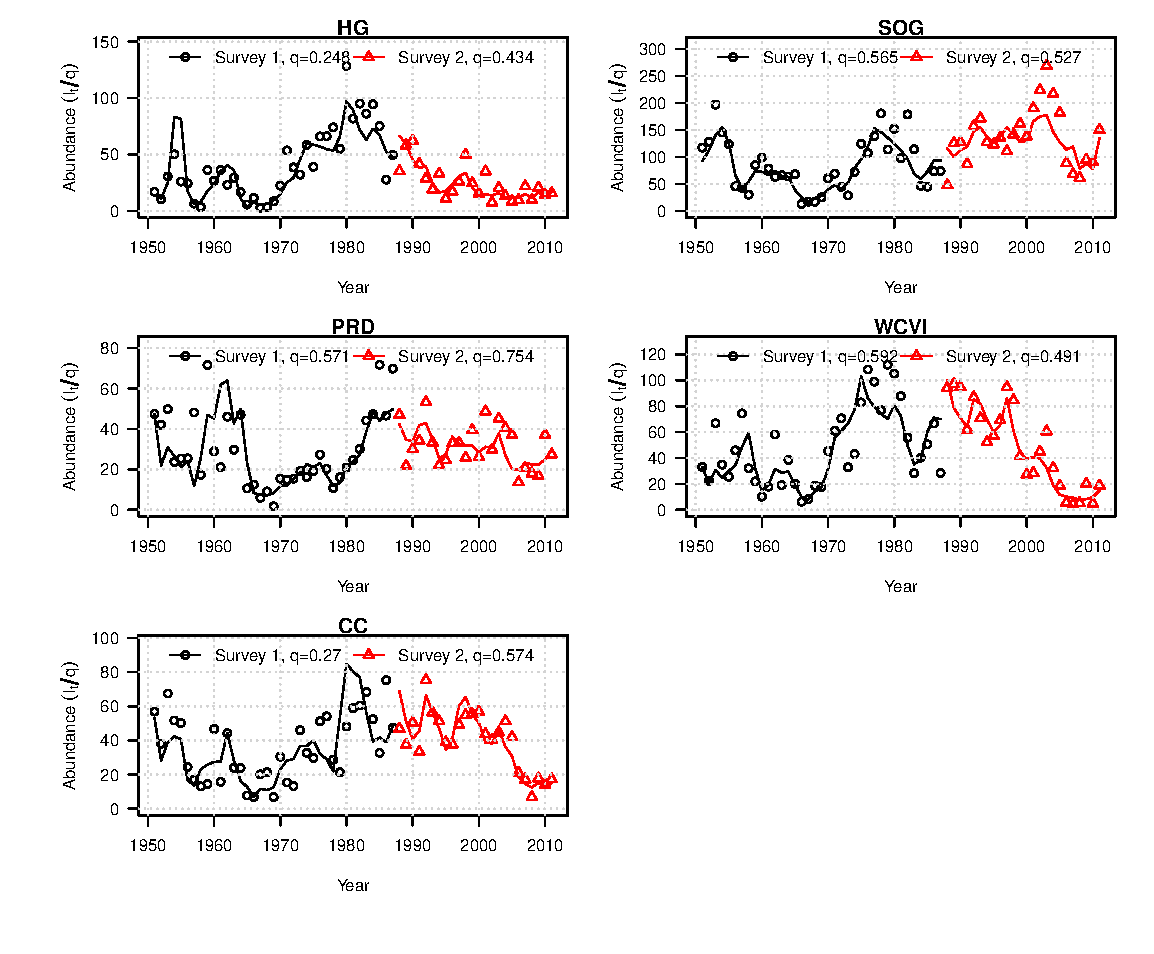
\includegraphics[width=\textwidth]{../FIGS/qPriorFigs/iscam_fig_surveyfit.pdf}\\
	\caption{Observed (points) and predicted (lines) spawn survey abundance data scaled by the MLE estimate of $q$ for each of the five major SARs.  In each panel, the corresponding scaler ($q$) is presented for each of the surveys.}\label{PartII:Results:fig3}
\end{figure}


\subsubsection{Age composition residuals}

The assumed error distribution for the age-composition data has changed in this assessment from a multinomial distribution implemented in HCAM to a multivariate-logistic distribution. In the former implementation the age-composition data were weighted by the annual samples sizes in each region for each age and year. In the \iscam\ implementation the age-composition data for all years is given the same weight (i.e., we assume the observation errors is homogenous) based on the conditional maximum likelihood estimate of the variance (see Appendix \ref{appiSCAM} for full details).  We further pool age-proportions that are less than 2\% into the adjacent younger year class to reduce the influence of small outliers and weak cohorts.

In HG the MLE estimates of the variance for each gear is 0.102, 0.106 and 0.306, for the winter seine, seine-roe and gillnet fleets, respectively (Fig. \ref{PartII:Results:figAgeCompHG}).  In general there is fairly good agreement between the observed and predicted age-composition data in this region, with poorer fits to the gillnet age-composition data.  There is no persistent pattern in the residuals. 

\begin{sidewaysfigure}[!tbp]
	% Requires \usepackage{graphicx}
	\centering
	\includegraphics[width=0.9\textwidth]{../FIGS/qPriorFigs/iscam_fig_agecompsresid_HG.pdf}\\
	\caption{Residual difference between the observed and predicted proportions-at-age for HG for each of the three gear types (Gear 1 = winter seine, Gear 2 = seine-roe, Gear 3 = gillnet).  The area of each circle is proportional to the residua, black is positive, and red is negative.  The corresponding MLE estimates of the residual variance is displayed in each panel.}\label{PartII:Results:figAgeCompHG}
\end{sidewaysfigure}

For the PRD region, the fits to the age-composition data are slightly poorer, with MLE estimates of the variance ranging from 0.164 to 0.269 for the gillnet and winter seine fleets (Fig. \ref{PartII:Results:figAgeCompPRD}). There is no remarkable pattern in the winter seine fishery, the seine-roe fishery tends to have positive residuals for age-3 and age 7+ fish, and negative residuals for ages 5-6 fish. Residuals in the gillnet fishery are mostly negative for age-4 fish post 1988. The gillnet gear tends to catch older fish than both seine gears.

\begin{sidewaysfigure}[!tbp]
	% Requires \usepackage{graphicx}
	\centering
	\includegraphics[width=0.9\textwidth]{../FIGS/qPriorFigs/iscam_fig_agecompsresid_PRD.pdf}\\
	\caption{Residual difference between the observed and predicted proportions-at-age for PRD for each of the three gear types (Gear 1 = winter seine, Gear 2 = seine-roe, Gear 3 = gillnet).  The area of each circle is proportional to the residua, black is positive, and red is negative.  The corresponding MLE estimates of the residual variance is displayed in each panel.}\label{PartII:Results:figAgeCompPRD}
\end{sidewaysfigure}


For the Central Coast (CC) region, there is also good correspondence between the observed and predicted age-composition data, with MLE estimates of the variance ranging from 0.135 to 0.201 (Fig. \ref{PartII:Results:figAgeCompCC}).  There is no striking temporal pattern in the residuals for any of the fishing fleets.  There is a tendency to overestimate the proportion-at-age 4 in the seine-roe fishery.


\begin{sidewaysfigure}[!tbp]
	% Requires \usepackage{graphicx}
	\centering
	\includegraphics[width=0.9\textwidth]{../FIGS/qPriorFigs/iscam_fig_agecompsresid_CC.pdf}\\
	\caption{Residual difference between the observed and predicted proportions-at-age for CC for each of the three gear types (Gear 1 = winter seine, Gear 2 = seine-roe, Gear 3 = gillnet).  The area of each circle is proportional to the residua, black is positive, and red is negative.  The corresponding MLE estimates of the residual variance is displayed in each panel.}\label{PartII:Results:figAgeCompCC}
\end{sidewaysfigure}

For the Strait of Georgia, there is also very good correspondence between the observed and predicted age-composition data for all three gears (Fig \ref{PartII:Results:figAgeCompSOG}).  The MLE estimates of the variance range from 0.089 to 0.263 for the seine-roe and winter seine fleets, respectively.  In the gillnet fleet  there has been a tendency to under-estimate the proportions-at-age 6-7 between the 1996 to 2011. Recall that selectivity for the gillnet fishery can be influenced by the empirical weight-at-age data, which has been trending to small fish in recent years.  In this case, the age-composition data do not suggest that changes in mean weight-at-age has influenced the selectivity patterns (see results for selectivities).


\begin{sidewaysfigure}[!tbp]
	% Requires \usepackage{graphicx}
	\centering
	\includegraphics[width=0.9\textwidth]{../FIGS/qPriorFigs/iscam_fig_agecompsresid_SOG.pdf}\\
	\caption{Residual difference between the observed and predicted proportions-at-age for SOG for each of the three gear types (Gear 1 = winter seine, Gear 2 = seine-roe, Gear 3 = gillnet).  The area of each circle is proportional to the residua, black is positive, and red is negative.  The corresponding MLE estimates of the residual variance is displayed in each panel.}\label{PartII:Results:figAgeCompSOG}
\end{sidewaysfigure}

In the case of WCVI, there is good correspondence between the observed and predicted age composition data for the seine fisheries and less so for the gillnet fishery (Fig \ref{PartII:Results:figAgeCompWCVI}).  The MLE estimates of the variance range from 0.092 to 0.237 for the seine-roe and gillnet fisheries, respectively.  Residual patterns in the seine fisheries and gillnet fisheries are unremarkable.   The size of the residuals are fairly homogenous over time for all gears.


\begin{sidewaysfigure}[!tbp]
	% Requires \usepackage{graphicx}
	\centering
	\includegraphics[width=0.9\textwidth]{../FIGS/qPriorFigs/iscam_fig_agecompsresid_WCVI.pdf}\\
	\caption{Residual difference between the observed and predicted proportions-at-age for WCVI for each of the three gear types (Gear 1 = winter seine, Gear 2 = seine-roe, Gear 3 = gillnet).  The area of each circle is proportional to the residua, black is positive, and red is negative.  The corresponding MLE estimates of the residual variance is displayed in each panel.}\label{PartII:Results:figAgeCompWCVI}
\end{sidewaysfigure}







\subsection{Biomass estimates \& reference points}

Maximum likelihood estimates of total biomass (age 2+) and the spawning stock biomass for each of the five major assessment regions in summarized in Figure \ref{PartII:Results:figBiomass}.  Estimates of spawning stock depletion ($B_t/B_0$) for the five major regions is summarized in Figure \ref{PartII:Results:figDepletion} along with estimates of the sustainable fisheries framework reference points.  With the exceptions of CC and WCVI, estimates of spawning stock depletion in 2011 are all currently at or above 40\% of their estimated unfished state. In the  CC and WCVI, spawning stock depletion is estimated to be  25\% and 25\% of their unfished state, respectively (Fig \ref{PartII:Results:figDepletion}).

Maximum likelihood estimates of spawning stock biomass in 2011 were as follows: HG -- 16,723 tonnes, PRD -- 27,288 tonnes, CC -- 14,624 tonnes, SOG -- 129,070 tonnes, and WCVI -- 14,909 tonnes (Table \ref{PartII:Table1:referencePoints}).  These estimates are considerably higher in comparison to last years HCAM estimates; the difference largely owes to the substantial change in spawn survey scaling coefficient ($q$).

In addition to the current estimates of spawning biomass, Table \ref{PartII:Table1:referencePoints} also summarizes estimates of reference points and the total number of estimated parameters for each of the five major stock assessment regions.  Each region contained data from 1951 to 2011, and the number of estimated parameters ranges from 159 in HG to 235 in SOG.  The difference in the number of estimated parameters owes to the difference in the number of years of catch data for each region.

Estimates of unfished spawning biomass for each region is as follows: HG -- 40,684 tonnes, PRD -- 68,761 tonnes, CC -- 59,365 tonnes, SOG -- 135,523 tonnes, and WCVI -- 57,462 tonnes.  Applying the same cutoff rule used in previous assessments (25\% of $B_0$), results in a substantial change in the cutoff levels for PRD, CC, SOG, and WCVI.  The previoucutoffs cutoff level for HG was estimated at 10,700 tonnes, and in this assessment there is a minor downward revision to 10,171 tonnes.  In the case of PRD, the previous cutoff was 12,100 tonnes and in this assessment is now 17,190 tonnes.  For the CC, the previous cutoff was 17,600 tonnes and now 14,841 tonnes.  For the SOG, the previous cutoff was 21,200 tonnes, and in this assessment it has been revised upwards to 33,881 tonnes.  Lastly, for the WCVI the cutoff has decreased from 18,800 tonnes to 14,366 tonnes. Note however, that these revised \bo's and cutoffs are Maximum Likelihood Estimates (MLE) and not median values from the joint posterior distribution (see section \ref{Section:Forecast})


% latex.default(rpTable, file = fn, rowname = NULL, longtable = FALSE,      landscape = FALSE, cgroup = NULL, n.cgroup = NULL, caption = cap,      label = "TableRefPoints", na.blank = TRUE, vbar = FALSE,      size = "small") 
%
\begin{table}[!tbp]
 \small
 \caption{Reference points\label{TableRefPoints}} 
 \begin{center}
 \begin{tabular}{llllllllll}\hline\hline
\multicolumn{1}{c}{Stock}&\multicolumn{1}{c}{No.}&\multicolumn{1}{c}{\fmsy}&\multicolumn{1}{c}{MSY}&\multicolumn{1}{c}{$B_0$}&\multicolumn{1}{c}{0.25$B_0$}&\multicolumn{1}{c}{\bmsy}&\multicolumn{1}{c}{0.8\bmsy}&\multicolumn{1}{c}{0.4\bmsy}&\multicolumn{1}{c}{Spawn depletion}\tabularnewline
\hline
HG&158&  2.68& 8,817&40,960&10,240& 8,776& 7,020& 3,510&  0.41\tabularnewline
PRD&205&  0.63& 6,658&80,247&20,062&18,911&15,128& 7,564&  0.23\tabularnewline
CC&189&   1.3& 7,844&56,181&14,045&10,765& 8,612& 4,306&   0.2\tabularnewline
SOG&234&   1.54& 22,786&116,023& 29,006& 23,161& 18,529&  9,264&   0.62\tabularnewline
WCVI&173&  1.03& 9,041&51,379&12,845&10,068& 8,054& 4,027&  0.23\tabularnewline
\hline
\end{tabular}

\end{center}

\end{table}




\begin{figure}[!tbp]
	% Requires \usepackage{graphicx}
	\includegraphics[width=\textwidth]{../FIGS/qPriorFigs/iscam_fig_biomass.pdf}\\
	\caption{Estimates of total biomass at the start of the year (numbers times empirical weight-at-age) and spawning stock biomass (post fishery) for the five major SARs.}\label{PartII:Results:figBiomass}
\end{figure}


\begin{figure}[!tbp]
	% Requires \usepackage{graphicx}
	\includegraphics[width=\textwidth]{../FIGS/qPriorFigs/iscam_fig_depletion.pdf}\\
	\caption{Estimates of spawning biomass depletion ($B_t/B_0$) for each of the five major stock areas.  Horizontal dotted lines represent 25\% and 40\% depletion levels, and the shaded regions demarcate reference points based on $<$40\% \bmsy/\bo (critical zone) and 40--80\% \bmsy/\bo(cautious zone) and $>$80\% \bmsy/\bo (healthy zone). Note that in calculating the \bmsy\ reference points, the average catch ratios over the last 20 years was used to partition fishing mortality to each of the gears.}\label{PartII:Results:figDepletion}
\end{figure}




\subsection{Estimates of mortality}

The most recent HCAM assessment model allowed for annual estimates of $M_t$ where natural mortality was modelled as a random walk process.  The same random walk model has been adopted in this \iscam\ implementation; however, a reduced number of parameters (12 nodes instead of 60 annual deviations) was estimated and interpolated using a bicubic spline.  The number of estimated nodes does have minor influences on the various trends in natural mortality; we came to arrive at estimating 12 nodes by ensuring the estimated trends were very similar to trends in $M$ when estimating 60 annual natural mortality rate deviations (NB. the use of formal model selection criterion should be used to determine the optimal number of nodes).

For all of the five major stock assessment regions, estimates of natural mortality rates have trended upwards since the 1950s (Figure \ref{PartII:Results:figMortality}).  Trends in estimates of natural mortality are also consistent with the trends in natural mortality from last years HCAM model  \citep[see Figure 18 in][]{Clear2010}.  There was no relationship between trends in natural mortality and trends in the empirical mean weight-at-age data.  Information about natural mortality comes from the age-composition data; therefore, changes in natural mortality rates over time is not necessarily linked with changes in growth rates, and vice versa.   In the mid to late 1970s, estimates of natural mortality rates were very low during a time when most of the stocks were recovering from the earlier reduction fishery.  In the last decade, estimates of natural mortality rates for herring have been at an all time high, and in all locations there is indication that natural mortality rates may be starting to decline. Estimates of $M_t$ in the most recent years, however,  are highly suspect because there are incomplete cohorts to infer estimates of total mortality rates and $M_t$ is also confounded with selectivity.



\begin{figure}[!tbp]
	% Requires \usepackage{graphicx}
	\includegraphics[width=\textwidth]{../FIGS/qPriorFigs/iscam_fig_mortality.pdf}\\
	\caption{Maximum likelihood estimates of the components of average total mortality for each of the five major stock assessment regions. Note that the y-axis is plotted on a log scale, natural mortality (grey) is age-independent, fishing mortality is age-specific and the average fishing mortality rate over all age-classes is plotted here.}\label{PartII:Results:figMortality}
\end{figure}

Estimates of fishing mortality rates in each of the regions, between 1951 and 1970 were very high due to the reduction fishery by the winter purse seine (Gear 1).  After the fishery re-opened in the early 1970s fishing mortality rates have been greatly reduced and periodic since the early 1990s due to the implementation of a harvest control rule with target escapements (cutoffs).  Of notable exceptions are the fishing mortality rates for the gillnet fishery in PRD  and SOG have been substantially higher than other regions and consistently open each and every year (Fig. \ref{PartII:Results:figMortality}). Note that fishing mortality rates for each gear in Fig. \ref{PartII:Results:figMortality} reflect the average fishing mortality over all age-classes and are not comparable among gears due to differences in gear selectivity. Fishing mortality rates for the gillnet fishery tend to be higher than the seine-roe fishery because recruitment to the gillnet gear is much older in comparison to the seine-roe gear.





\subsection{Selectivity}

Maximum likelihood estimates of selectivity for the winter seine fishery, seine-roe fishery and the gillnet fishery for each of the five major SARs are shown in Figures \ref{PartII:Results:figWinterSeineSel}, \ref{PartII:Results:figSeineRoeSel}, and \ref{PartII:Results:figGillNetSel}, respectively.  Selectivities for the seine fisheries were assumed time-invariant, and selectivity for the gillnet fishery varies over time due to changes in the mean weight-at-age data.

For the winter seine fishery, age-specific selectivity coefficients were somewhat variable among the assessment regions (Fig. \ref{PartII:Results:figWinterSeineSel}).  The age at which herring were fully recruited to the gear was roughly age 5 for CC, SOG, and WCVI.  Age at full recruitment for HG and PRD was much older, 9- and 10-years, respectively.


\begin{figure}[!tbp]
	% Requires \usepackage{graphicx}
	\includegraphics[width=\textwidth]{../FIGS/qPriorFigs/iscam_fig_sel2d_winter_seine_sel.pdf}\\
	\caption{Maximum likelihood estimates of age-specific selectivity coefficients for the winter seine fishery for each of the major stock areas.}\label{PartII:Results:figWinterSeineSel}
\end{figure}

For the seine-roe fishery, maximum likelihood estimates of selectivity were much more consistent among regions than the winter seine fishery (Fig. \ref{PartII:Results:figSeineRoeSel}).  Age at full recruitment to this gear type was roughly 5-6 years, and roughly the age at 50\% vulnerability was roughly 3-4 years, with a tendency to recruit to the fishery at a younger age in the southern regions.

\begin{figure}[!tbp]
	% Requires \usepackage{graphicx}
	\includegraphics[width=\textwidth]{../FIGS/qPriorFigs/iscam_fig_sel2d_seine_roe_sel.pdf}\\
	\caption{Maximum likelihood estimates of age-specific selectivity coefficients for the seine-roe fishery for each of the major stock areas.}\label{PartII:Results:figSeineRoeSel}
\end{figure}

In the case of the gillnet fishery, selectivity was allowed to vary over time according to variation in the empirical weight-at-age data (Fig. \ref{PartII:Results:figGillNetSel}).  Recall that selectivity for the gillnet fishery was modelled as a logistic function of age with the addition of age-specific deviations where selectivity can increase if the weight-at-age is above average for that year.  This selectivity function consists of three latent variables: two that describe the age-at-50\% vulnerability and standard deviation in vulnerability-at-age, and a third parameter that describes the influence of variation in weight-at-age on departures from the logistic selectivity function ($\lambda^{(a)}$).  Maximum likelihood estimates for these parameters for the gillnet fishery are presented in Table \ref{PartII:Table:GN_Sel_par}.  With the exception of PRD and WCVI, estimates of $\lambda^{(a)}$ are negative and close to 0 implying no affect of variation in weight-at-age on selectivity or a slight negative effect (i.e., vulnerability to the gear declines for fish that are larger than the average weight).  In the case of PRD and WCVI, the variation in weight-at-age explains approximately 4.1\% and 8.7\% of the residual variation in the age-composition data (Table \ref{PartII:Table:GN_Sel_par}).

\begin{figure}[!tbp]
	% Requires \usepackage{graphicx}
	\includegraphics[width=\textwidth]{../FIGS/qPriorFigs/iscam_fig_gill_net_selectivity.pdf}\\
	\caption{Estimates of selectivity for the gillnet fleet for each of the five major stock assessment regions. In this case selectivity is a logistic function of the empirical weight-at-age data; due to declining growth there is a tendency for selectivity to shift to older ages.}\label{PartII:Results:figGillNetSel}
\end{figure}


%% Insert table here with estimates of selectivity parameters.
\begin{table}[htdp]
\caption{Maximum likelihood estimates of gillnet selectivity parameters, where $\mu_a$ is the age-at-50\% vulnerability, $\sigma_a$ is the standard deviation in selectivity, and $\lambda^{(a)}$ is the coefficient that describes the influence of growth on selectivity ($\lambda^{(a)}$=0 implies no effect, $\lambda^{(a)}>0$ implies a positive effect).}
\begin{center}
\begin{tabular}{lcccc}
\hline
Stock 	& $\ln(\mu_a)$ 	& $\ln(\sigma_a)$	& $\lambda^{(a)}$ &$\sigma_{\lambda^{(a)}}$\\
\hline
HG		&	 1.598		&	-0.68125		&	-0.030581 &	0.045 \\
PRD		&    1.727		&   -0.66217		&    0.040988 & 0.108 \\
CC		&    1.604 		&   -0.8050        &   -0.019404  & 0.028 \\
SOG		&	 1.540		&   -0.9797			&   -0.02835  & 0.068 \\
WCVI	& 	 1.608		&   -0.6647			& 	 0.08677  & 0.014\\
\hline
\end{tabular}
\end{center}
\label{PartII:Table:GN_Sel_par}
\end{table}%


%%%%%%%%%%%%%%%%%%%%%%%%%%%%%%%%%%%%%%%%%%%%%%%%%%%%%%%%%%%%%%%
%%%%%%%%%%%%%%%%%%%%%%%%%%%%%%%%%%%%%%%%%%%%%%%%%%%%%%%%%%%%%%%
\subsection{Recruitment and stock-recruitment relationships}

Recruitment to each stock is defined as the number of age-2 fish entering the population at the beginning of each year (i.e., May 1). Age-2 recruitment is estimated as a free parameter within \iscam, subject to the constraint that annual estimates vary around a Beverton-Holt stock recruitment relationship with an estimated unknown standard deviation.  Maximum likelihood estimates of age-2 recruits are shown in Figure \ref{PartII:Results:FigAge2Recruits} along with horizontal lines that demarcate the 0.33 and 0.66 quantiles that was traditionally used to categorize recruitment as poor, average, and good in previous assessments.

Estimates of age-2 recruits for 2010 and 2011 were average and good  in HG, average in PRD, good and average in CC, good in SOG, and average and poor in the WCVI region.  Note however, that estimates of age-2 recruits are highly uncertain in the most recent years of a stock assessment because these age-classes are only partially recruited to the fishing gears.


\begin{figure}[!tbp]
	% Requires \usepackage{graphicx}
	\includegraphics[width=\textwidth]{../FIGS/qPriorFigs/iscam_fig_recruitment.pdf}\\
	\caption{Maximum likelihood estimates of age-2 recruits for each of the five major stock areas and the asymptotic estimates of the 95\% confidence interval.  The horizontal divisions demarcate the 0.33 and 0.66 quantiles that define poor, average, and good recruitment.}\label{PartII:Results:FigAge2Recruits}
\end{figure}

The underlying stock-recruitment relationship is key for determining reference points for this stock.  Maximum likelihood estimates of the age-2 recruits versus spawning biomass, along with the corresponding Beverton-Holt stock recruitment model are shown in Figure \ref{PARTII:Results:FigStockRecruit}.  The Beverton-Holt stock recruitment model was jointly fitted to these data by estimating the steepness of the stock recruitment relationship ($h$) and the unfished age-2 recruits ($R_0$).  The unfished spawning biomass was determined by using the average fecundity and average natural mortality rates (from 1951-2011) to calculate the average spawning biomass per recruit. Alternative stock-recruitment models (e.g., Ricker model) were not explored to determine if they provided a better fit.



\begin{figure}[!tbp]
	% Requires \usepackage{graphicx}
	\includegraphics[width=\textwidth]{../FIGS/qPriorFigs/iscam_fig_stockrecruit.pdf}\\
	\caption{Maximum likelihood estimates of age-2 recruits versus estimated spawning stock biomass in each of the five major assessment regions.  The green and red circles indicate the start (recruits in 1952) and end (recruits in 2011) of the series, the circle plus (red) corresponds to the maximum likelihood estimate of unfished spawning biomass (\bo) and unfished age-2 recruitment $R_0$, the line is the Beverton-Holt stock recruitment model fitted to these data. }\label{PARTII:Results:FigStockRecruit}
\end{figure}

Between 1951 and 2011, four of the five major stock areas have fluctuated above the estimate of unfished spawning biomass; the exception is the PRD area.  In HG, age-2 recruitment has been remarkably stable over a very wide range of spawner abundance. This is also the case for CC and WCVI.  In PRD and SOG, variation in recruitment appears to be lower at low spawning abundance and the average recruitment rate tends to drop.  Maximum likelihood estimates for steepness for these five stocks are as follows: HG -- 0.81, PRD -- 0.66, CC -- 0.82, SOG -- 0.76, WCVI -- 0.77.

The log residual differences between the estimated age-2 recruits and that predicted by the estimated spawning-biomass and Beverton-Holt model for each of the major stock areas is shown in Figure \ref{PartII:Results:RecResiduals}.  There is no strong autocorrelation in recruitment, except perhaps 5-8 year periods of poor and good recruitment in SOG.  There is good correspondence between the standard deviations of the residuals and the estimated standard deviation of the process error variance ($\tau$).

\begin{figure}[!tbp]
	% Requires \usepackage{graphicx}
	\includegraphics[width=\textwidth]{../FIGS/qPriorFigs/iscam_fig_recresid.pdf}\\
	\caption{Log residual differences between estimated age-2 recruits and the recruitment predicted by the Beverton-Holt model and estimated spawning stock biomass.  The standard deviations of the residuals along with the MLE estimate of the process error standard deviations are displayed at the top of each panel.}\label{PartII:Results:RecResiduals}
\end{figure}
%%%%%%%%%%%%%%%%%%%%%%%%%%%%%%%%%%%%%%%%%%%%%%%%%%%%%%%%%%%%%%%
%%%%%%%%%%%%%%%%%%%%%%%%%%%%%%%%%%%%%%%%%%%%%%%%%%%%%%%%%%%%%%%
\subsection{Retrospective analysis}
Four of the five major regions contained little to no retrospective bias in the estimates of spawning stock biomass when fitting the data back to 2001 (10 years, Figure \ref{fig:PartII:sbRetrospective}).  The PRD region does show a strong retrospective bias; as each year of data is removed estimates of the terminal spawning biomass that year increase.  This pattern of declining estimates of biomass as data are added is persistent for all of the years in which the retrospective estimates were examined which implies that estimates of biomass in this region are positively biased.  The direction of bias in PRD warrants extra caution as uncertainty in biomass estimates are also likely biased upwards.

In SOG, there was no retrospective bias; however, there is some retrospective error that occurs when data from 2008 and onwards are removed from the analysis. Information in the data prior to 2008 suggest large increases in spawning abundance in the early 2000s.  This increase is revised downwards when the 2008 data are included in the assessment.  It is not clear what components of the data suggest this downward revision.  

Key to the harvest control rule is the estimate of unfished spawning biomass in each of the SARs.  The points plotted in Figure \ref{fig:PartII:sbRetrospective} show how estimates of $B_o$ change as more data accumulates over time.  If estimates of $B_o$ increase over time, then cuttoff levels would also increase, and vice versa.  In all regions with the exception of PRD, retrospective estimates of $B_o$ have been relatively consistent and trending downwards slightly as more and more data have accumulated over time.  Retrospecitve estimates of $B_o$ in PRD are much more variable in comparison to other areas. A more conservative policy would be to set cutoff levels an the upper end of the $B_o$ estimates for this region.


\begin{figure}[!tbp]
	% Requires \usepackage{graphicx}
	\includegraphics[width=\textwidth]{../FIGS/qPriorFigs/iscam_fig_sbt_retrospective.pdf}\\
	\caption{Retrospective estimates of spawning stock biomass and estimates of unfished biomass ($B_o$ shown as circles) for each of the five major stock assessment areas.  The model was sequentially fitted to the full data set, then from 1951:2010, 1951:2009, ... 1951:2001.}\label{fig:PartII:sbRetrospective}
\end{figure}


%%%%%%%%%%%%%%%%%%%%%%%%%%%%%%%%%%%%%%%%%%%%%%%%%%%%%%%%%%%%%%%
%%%%%%%%%%%%%%%%%%%%%%%%%%%%%%%%%%%%%%%%%%%%%%%%%%%%%%%%%%%%%%%
\subsection{Marginal posterior distributions}
Marginal posterior distributions for estimated model parameters were constructed using AD Model Builders built in Metropolis-Hastings algorithm \citep{gelman2004bayesian}.  For each of the major and minor assessment areas, a systematic sample of 2,000 points from a chain of length 1,000,000 and is intended to represent a random sample from the joint posterior distribution.  These samples were then used to construct marginal distributions for derived quantities (e.g., \bo).  All areas with the exception of the SOG used the inverse Hessian matrix as the jumping distribution.  In the case of SOG, the hessian matrix had to be re-scaled (using the \texttt{-mcmult 2.0} option in ADMB) in order to invert the Hessian matrix.


\subsubsection{Diagnostic trace plots}

No formal  statistical tests were carried out to determine if the samples from the joint posterior distribution were taken from a converged distribution.  Visual inspection was used to determine overall convergence and the trace plots for each of the five major regions are shown in Figures \ref{PartII:MCMC:traceHG}--\ref{PartII:MCMC:traceWCVI}.

\begin{sidewaysfigure}[!tbp]
	% Requires \usepackage{graphicx}
	\centering
	\includegraphics[width=0.9\textwidth]{../FIGS/qPriorFigs/iscam_fig_trace_HG.pdf}\\
	\caption{A systematic sample of 2,000 from an MCMC chain of length 1,000,000 of leading parameters and derived variables used in reference point calculations for HG. Green circle corresponds to the MLE estimates and the solid line is a lowess smooth fit to the data (f=1/4), and the dashed line is the mean of the distribution.}\label{PartII:MCMC:traceHG}
\end{sidewaysfigure}


\begin{sidewaysfigure}[!tbp]
	% Requires \usepackage{graphicx}
	\includegraphics[width=0.9\textwidth]{../FIGS/qPriorFigs/iscam_fig_trace_PRD.pdf}\\
	\caption{A systematic sample of 2,000 from an MCMC chain of length 1,000,000 of leading parameters and derived variables used in reference point calculations for PRD. Green circle corresponds to the MLE estimates and the solid line is a lowess smooth fit to the data (f=1/4), and the dashed line is the mean of the distribution.}\label{PartII:MCMC:tracePRD}
\end{sidewaysfigure}

\begin{sidewaysfigure}[!tbp]
	% Requires \usepackage{graphicx}
	\includegraphics[width=0.9\textwidth]{../FIGS/qPriorFigs/iscam_fig_trace_CC.pdf}\\
	\caption{A systematic sample of 2,000 from an MCMC chain of length 1,000,000 of leading parameters and derived variables used in reference point calculations for CC. Green circle corresponds to the MLE estimates and the solid line is a lowess smooth fit to the data (f=1/4), and the dashed line is the mean of the distribution.}\label{PartII:MCMC:traceCC}
\end{sidewaysfigure}

\begin{sidewaysfigure}[!tbp]
	% Requires \usepackage{graphicx}
	\includegraphics[width=0.9\textwidth]{../FIGS/qPriorFigs/iscam_fig_trace_SOG.pdf}\\
	\caption{A systematic sample of 2,000 from an MCMC chain of length 1,000,000 of leading parameters and derived variables used in reference point calculations for SOG. Green circle corresponds to the MLE estimates and the solid line is a lowess smooth fit to the data (f=1/4), and the dashed line is the mean of the distribution.}\label{PartII:MCMC:traceSOG}
\end{sidewaysfigure}

\begin{sidewaysfigure}[!tbp]
	% Requires \usepackage{graphicx}
	\includegraphics[width=0.9\textwidth]{../FIGS/qPriorFigs/iscam_fig_trace_WCVI.pdf}\\
	\caption{A systematic sample of 2,000 from an MCMC chain of length 1,000,000 of leading parameters and derived variables used in reference point calculations for WCVI. Green circle corresponds to the MLE estimates and the solid line is a lowess smooth fit to the data (f=1/4), and the dashed line is the mean of the distribution.}\label{PartII:MCMC:traceWCVI}
\end{sidewaysfigure}


\subsection{Parameter confounding}

To examine the level of confounding among the estimated parameters, 200 randomly selected points from the joint posterior distribution for the seven leading parameters were plotted against each other in a pairs plot (e.g., Fig. \ref{PartII:MCMC:pairsHG}). Only 200 points were plotted to reduce the file size.   Among the seven leading estimated parameters ($R_0,h,M,\bar{R},\ddot{R}, \rho, \vartheta$) there was very little confounding (Figures \ref{PartII:MCMC:pairsHG} -- \ref{PartII:MCMC:pairsWCVI}).

There is, however, some strong confounding between the estimated parameters and a few of the derived reference points.  In all major areas, there was a strong positive correlation between steepness ($h$) and \fmsy; similarly there is a strong positive correlation between \bo and $R_0$.  Among the reference points alone, there is a negative correlation between \bmsy\ and \fmsy, and a positive correlation between \fmsy\ and MSY.  This level of confounding among the derived variables is not cause for concern  from a parameter estimation standpoint; it does, however,  highlight the tradeoffs that must be made from a decision makers perspective.


\begin{figure}[!tbp]
	% Requires \usepackage{graphicx}
	\includegraphics[width=\textwidth]{../FIGS/qPriorFigs/iscam_fig_pairs_HG.pdf}\\
	\caption{Pairs plot and marginal distributions for leading parameters in HG region (200 random samples).  The dotted lines correspond to the means of the distributions, circle is the mean, and the red square is the mode of the distribution.}\label{PartII:MCMC:pairsHG}
\end{figure}


\begin{figure}[!tbp]
	% Requires \usepackage{graphicx}
	\includegraphics[width=\textwidth]{../FIGS/qPriorFigs/iscam_fig_pairs_PRD.pdf}\\
	\caption{Pairs plot and marginal distributions for leading parameters in PRD region (200 random samples).  The dotted lines correspond to the means of the distributions, circle is the mean, and the red square is the mode of the distribution.}\label{PartII:MCMC:pairsPRD}
\end{figure}

\begin{figure}[!tbp]
	% Requires \usepackage{graphicx}
	\includegraphics[width=\textwidth]{../FIGS/qPriorFigs/iscam_fig_pairs_CC.pdf}\\
	\caption{Pairs plot and marginal distributions for leading parameters in CC region (200 random samples).  The dotted lines correspond to the means of the distributions, circle is the mean, and the red square is the mode of the distribution.}\label{PartII:MCMC:pairsCC}
\end{figure}

\begin{figure}[!tbp]
	% Requires \usepackage{graphicx}
	\includegraphics[width=\textwidth]{../FIGS/qPriorFigs/iscam_fig_pairs_SOG.pdf}\\
	\caption{Pairs plot and marginal distributions for leading parameters in SOG region (200 random samples).  The dotted lines correspond to the means of the distributions, circle is the mean, and the red square is the mode of the distribution.}\label{PartII:MCMC:pairsSOG}
\end{figure}

\begin{figure}[!tbp]
	% Requires \usepackage{graphicx}
	\includegraphics[width=\textwidth]{../FIGS/qPriorFigs/iscam_fig_pairs_WCVI.pdf}\\
	\caption{Pairs plot and marginal distributions for leading parameters in WCVI region (200 random samples).  The dotted lines correspond to the means of the distributions, circle is the mean, and the red square is the mode of the distribution.}\label{PartII:MCMC:pairsWCVI}
\end{figure}

%%%%%%%%%%%%%%%%%%%%%%%%%%%%%%%%%%%%%%%%%%%%%%%%%%%%%%%%%%%%%%%
%%%%%%%%%%%%%%%%%%%%%%%%%%%%%%%%%%%%%%%%%%%%%%%%%%%%%%%%%%%%%%%
\subsection{Marginal posterior distributions}

Marginal posterior distributions and along with the prior densities for the seven leading parameters are shown in Figure \ref{PartII:MCMC:Marginals}. In all cases, the steepness parameter, followed by the instantaneous natural mortality rate appears to be the most influenced by the prior density. Uniform prior distributions were assumed for the scaling parameters ($R_0, \bar{R}$, and $\ddot{R}$).  There were good posterior updates for the total variance and variance portioning parameters ($\vartheta, \rho$).

\begin{figure}[!tbp]
	% Requires \usepackage{graphicx}
	\centering
	\setlength\fboxsep{0pt}
\setlength\fboxrule{0.5pt}
%\fbox{\includegraphics{chick}}
	\fbox{\includegraphics[width=0.49\textwidth]{../FIGS/qPriorFigs/iscam_fig_marginals_HG.pdf}}
	\fbox{\includegraphics[width=0.49\textwidth]{../FIGS/qPriorFigs/iscam_fig_marginals_PRD.pdf}}
	\fbox{\includegraphics[width=0.49\textwidth]{../FIGS/qPriorFigs/iscam_fig_marginals_CC.pdf}}
	\fbox{\includegraphics[width=0.49\textwidth]{../FIGS/qPriorFigs/iscam_fig_marginals_SOG.pdf}}
	\fbox{\includegraphics[width=0.49\textwidth]{../FIGS/qPriorFigs/iscam_fig_marginals_WCVI.pdf}}

	\caption{Marginal posterior densities (histograms) and prior densities (lines) for the seven leading parameters and spawn survey scaler ($\ln(q)$, tan colour) for each of the five major assessment regions. Note the x-axis range corresponds to the lower and upper bounds of each model parameter, and the number in the top right corner is the ratio of posterior standard deviation to prior standard deviation (a ratio close to one implies no information in the data to estimate the parameter).}\label{PartII:MCMC:Marginals}
\end{figure}

Median estimates of the 2011 spawning stock biomass and the 95\% credible interval for each of the five major assessment regions are summarized in Table \ref{table:2011_SB_Depletion}.  Current estimates of depletion and the corresponding uncertainty is based on the ratio of the 2011 spawning biomass divided by the corresponding estimate of \bo.  Depletion levels less that 0.25 would be considered to be below the cutoff level.

\begin{table}
	\caption{Estimates of 2011 spawning biomass, $B_0$, and depletion based on 2000 systematic samples from the joint posterior distribution drawn from a chain of length 1,000,000.\label{table:2011_SB_Depletion}}
	\begin{center}
	\begin{small}
	\begin{tabular}{l>{\bfseries}ccc|>{\bfseries}ccc|>{\bfseries}ccc}
	\hline 
	&\multicolumn{3}{c}{$SB_{2011}$} 
	&\multicolumn{3}{c}{$B_0$} 
	&\multicolumn{3}{c}{$SB_{2011}/B_0$}\\
	Stock 
	&Median & 2.5\% & 97.5\%
	&Median & 2.5\% & 97.5\%
	&Median & 2.5\% & 97.5\% \\
	\hline
	HG & 16.58 & 7.70 &33.63& 41.74 &30.05 &61.51&  0.39  &0.19  &0.75 \\
	PRD & 27.05 & 14.45&  50.59 & 78.56 & 54.15 &150.18 &  0.34  & 0.15  & 0.68\\
	CC & 14.67 & 7.28 &27.28 &62.40& 48.47& 85.06 & 0.23 & 0.12 & 0.41\\
	SOG & 125.14 & 70.43& 217.95 &140.05& 110.47& 184.24 &  0.89 &  0.53 &  1.45\\
	WCVI & 14.68 & 6.99 &27.63& 59.58& 46.84& 78.53&  0.24 & 0.12&  0.43\\
	\hline
	\end{tabular}
	\end{small}
	\end{center}
\end{table}


%%%%%%%%%%%%%%%%%%%%%%%%%%%%%%%%%%%%%%%%%%%%%%%%%%%%%%%%%%%%%%%
%%%%%%%%%%%%%%%%%%%%%%%%%%%%%%%%%%%%%%%%%%%%%%%%%%%%%%%%%%%%%%%

\subsection{Forecast and catch advice based on the joint posterior distribution} \label{Section:Forecast}

Catch advice has historically been provided in the form of a decision table based on median values of the joint posterior distribution.  The decision table contains columns specifying the 2011 SSB the age 4+ total biomass, estimates of age-3 recruit biomass for poor, average, and good recruitment, cutoff levels, and the available harvest under poor, average, and good recruitment scenarios.  Moving towards DFO's sustainable fisheries framework  (SFF) is a necessary next step.  The SFF calls for the establishment of three reference levels: (1) the limit reference point (LRP) that defines the transition between the critical zone and the cautious zone, (2) and Upper Stock Reference (USR) that defines the transition between the cautious zone and the healthy zone, and (3) the Removal Reference (RR) which is the maximum removal rate when the stock is in the healthy zone \citep{shelton2008s}.  Suggested default levels for these reference levels are 0.4\bmsy\ and 0.8\bmsy\ for the LRP and USR, respectively and \fmsy\ for the RR.  At present these suggested reference points have not undergone simulation testing.  Moreover, the definition of MSY based reference points for this fishery require an \textit{a priori} allocation of the total catch to each of the different gears that harvest herring.  Finally, there is also a great deal of uncertainty associated with estimates of \bmsy for each of the SARs; probabilities of exceeding these reference points must also be established \textit{a priori} before we can move this fishery towards the sustainable fisheries framework.  

Cutoff levels for the BC herring stocks is defined as 0.25\bo. The historical cutoff levels have not been updated for over 10 years now (1996/1997).  Recent stock assessments (since 2001) for BC herring have assumed $q=1$ for the spawn survey data.  In this assessment we have relaxed this assumption and as a consequence estimates of herring biomass have increased substantially.  Due to significant changes in population scaling it would not make sense to continue to use the previous cutoff levels as this may lead to policies that would result in overfishing or under utilization of the resource.  We therefore present catch advice based on both the old cutoffs and the new cutoffs in Tables \ref{TableCatchAdviceOldCuttoffs}-\ref{TableCatchAdviceNewCuttoffs} for comparison. Under the new model and the median estimates of unfished biomass, cutoff levels decreased in HG, CC and the WCVI, and increased in PRD and the SOG.  In the case of SOG, cutoff values increased from 21,200 t to 35,013 t.  In PRD, cutoff values increased from 12,100 t to 19,641 t.  In both cases the catch advice based on the current HCR does not differ for the average and good recruitment scenarios as the projected 3+ biomass is well above these cutoff values.

% latex.default(xTable, file = fn, rowname = NULL, longtable = FALSE,      landscape = FALSE, cgroup = cgrp, n.cgroup = ncgrp, caption = cap,      label = "TableCatchAdvice", na.blank = TRUE, vbar = FALSE,      size = "small") 
%
\begin{table}[!tbp]
 \small
 \caption{Estimated spawning stock biomass,  age-4+ biomass and pre-fishery
			biomass for poor average and good recruitment, old cutoffs,  and 
			available harvest based on median values from the joint posterior distribution.\label{TableCatchAdviceOldCuttoffs}} 
 \begin{center}
 \begin{tabular}{lllclllclclll}\hline\hline
\multicolumn{3}{c}{\bfseries }&
\multicolumn{1}{c}{\bfseries }&
\multicolumn{3}{c}{\bfseries Pre-fishery forecast biomass}&
\multicolumn{1}{c}{\bfseries }&
\multicolumn{1}{c}{\bfseries }&
\multicolumn{1}{c}{\bfseries }&
\multicolumn{3}{c}{\bfseries Available harvest}
\tabularnewline \cline{1-13}
\multicolumn{1}{c}{Stock}&\multicolumn{1}{c}{SSB}&\multicolumn{1}{c}{4+ Biomass}&\multicolumn{1}{c}{}&\multicolumn{1}{c}{Poor}&\multicolumn{1}{c}{Average}&\multicolumn{1}{c}{Good}&\multicolumn{1}{c}{}&\multicolumn{1}{c}{Cutoff}&\multicolumn{1}{c}{}&\multicolumn{1}{c}{Poor}&\multicolumn{1}{c}{Average}&\multicolumn{1}{c}{Good}\tabularnewline
\hline
HG&16,579& 7,089&& 9,618&12,892&21,478&&10,700&&     0& 2,192& 4,296\tabularnewline
PRD&27,046&20,593&&24,150&27,492&37,286&&12,100&& 4,830& 5,498& 7,457\tabularnewline
CC&14,666& 7,809&&11,357&14,709&22,883&&17,600&&     0&     0& 4,577\tabularnewline
SOG&125,261& 72,937&& 94,703&112,856&138,448&& 21,200&& 18,941& 22,571& 27,690\tabularnewline
WCVI&14,679& 8,267&&15,321&20,906&31,130&&18,800&&     0& 2,106& 6,226\tabularnewline
\hline
\end{tabular}

\end{center}

\end{table}


% latex.default(xTable, file = fn, rowname = NULL, longtable = FALSE,      landscape = FALSE, cgroup = cgrp, n.cgroup = ncgrp, caption = cap,      label = "TableCatchAdvice", na.blank = TRUE, vbar = FALSE,      size = "small") 
%
\begin{table}[!tbp]
 \small
 \caption{Estimated spawning stock biomass,  
		age-4+ biomass and pre-fishery biomass 
		for poor average and good recruitment, 
		new cutoffs (based on median value of 0.25B$_0$
		estimated within the \iscam\ model), 
		and available harvest based on the median 
		values from the joint posterior distribution.\label{TableCatchAdviceNewCuttoffs}} 
 \begin{center}
 \begin{tabular}{lllclllclclll}\hline\hline
\multicolumn{3}{c}{\bfseries }&
\multicolumn{1}{c}{\bfseries }&
\multicolumn{3}{c}{\bfseries Pre-fishery forecast biomass}&
\multicolumn{1}{c}{\bfseries }&
\multicolumn{1}{c}{\bfseries }&
\multicolumn{1}{c}{\bfseries }&
\multicolumn{3}{c}{\bfseries Available harvest}
\tabularnewline \cline{1-13}
\multicolumn{1}{c}{Stock}&\multicolumn{1}{c}{SSB}&\multicolumn{1}{c}{4+ Biomass}&\multicolumn{1}{c}{}&\multicolumn{1}{c}{Poor}&\multicolumn{1}{c}{Average}&\multicolumn{1}{c}{Good}&\multicolumn{1}{c}{}&\multicolumn{1}{c}{Cutoff}&\multicolumn{1}{c}{}&\multicolumn{1}{c}{Poor}&\multicolumn{1}{c}{Average}&\multicolumn{1}{c}{Good}\tabularnewline
\hline
HG&16,579& 7,089&& 9,618&12,892&21,478&&10,436&&     0& 2,456& 4,296\tabularnewline
PRD&27,046&20,593&&24,150&27,492&37,286&&19,641&& 4,510& 5,498& 7,457\tabularnewline
CC&14,666& 7,809&&11,357&14,709&22,883&&15,600&&     0&     0& 4,577\tabularnewline
SOG&125,261& 72,937&& 94,703&112,856&138,448&& 35,013&& 18,941& 22,571& 27,690\tabularnewline
WCVI&14,679& 8,267&&15,321&20,906&31,130&&14,894&&   427& 4,181& 6,226\tabularnewline
\hline
\end{tabular}

\end{center}

\end{table}



In addition to Tables \ref{TableCatchAdviceOldCuttoffs} and \ref{TableCatchAdviceNewCuttoffs} we also provide an additional risk-based decision table that attempts to integrate over all of the uncertainty in the model (Tables \ref{Table:RiskCC}-\ref{Table:RiskWCVI}).  This decision table is also represented graphically in Figure \ref{fig:Risk}.  Figure \ref{fig:Risk} should be interpreted as follows: the probability of the spawning stock biomass falling below the cutoff level is determined by drawing a vertical line that intersect the cumulative probability curve and reading off the corresponding probability level. The reverse of this process was used to construct Tables \ref{Table:RiskCC}-\ref{Table:RiskWCVI}.
\clearpage
% latex.default(TAC, file = fn, title = "Risk", longtable = FALSE,      landscape = FALSE, cgroup = NULL, n.cgroup = NULL, caption = cap,      label = paste("Table:Risk", hdr$Stock[i], sep = ""), na.blank = TRUE,      vbar = FALSE) 
%
\begin{table}[!tbp]
 \caption{Decision table for HG where the risk 
			level represents the probability of exceeding the quantities specified
			in the headers of each column.  Three performance measures are considered:
			the probability of the spawning stock biomass in 2013 falling below the cutoff
			level,  the probability of the spawning stock biomass in 2013 declining from 2012, 
			and the probability of 2012 exploitation rate exceeding the 20\% level that is
			used in the harvest control rule. To use this table, first determine the 
			appropriate level of risk (e.g. 0.25 or 25\% chance),  then choose the appropriate
			management quantity (e.g. spawning biomass falling below the cutoff), and then read
			off the recommended catch (e.g.,  3,060 tonnes).\label{Table:RiskHG}} 
 \begin{center}
 \begin{tabular}{llll}\hline\hline
\multicolumn{1}{c}{Risk level}&\multicolumn{1}{c}{$P(SB_{2013})\textless$Cutoff}&\multicolumn{1}{c}{$P(SB_{2013}<SB_{2012})$}&\multicolumn{1}{c}{$P(U_{2012}<0.2)$}\tabularnewline
\hline
0.05&     0&     0& 2,228\tabularnewline
0.1&     0&     0& 3,552\tabularnewline
0.15&   583&     0& 4,372\tabularnewline
0.2& 1,940&     0& 4,989\tabularnewline
0.25& 3,060&     0& 5,498\tabularnewline
0.3& 4,039&     0& 5,944\tabularnewline
0.35& 4,928&     0& 6,348\tabularnewline
0.4& 5,760&     0& 6,727\tabularnewline
0.45& 6,558&     0& 7,090\tabularnewline
0.5& 7,340&     0& 7,445\tabularnewline
0.55& 8,121&     0& 7,801\tabularnewline
0.6& 8,919&   907& 8,164\tabularnewline
0.65& 9,751& 2,547& 8,542\tabularnewline
0.7&10,640& 4,299& 8,947\tabularnewline
0.75&11,619& 6,229& 9,392\tabularnewline
0.8&12,740& 8,439& 9,902\tabularnewline
0.85&14,096&11,113&10,519\tabularnewline
0.9&15,898&14,666&11,338\tabularnewline
0.95&18,809&20,404&12,662\tabularnewline
\hline
\end{tabular}

\end{center}

\end{table}


% latex.default(TAC, file = fn, title = "Risk", longtable = FALSE,      landscape = FALSE, cgroup = NULL, n.cgroup = NULL, caption = cap,      label = paste("Table:Risk", hdr$Stock[i], sep = ""), na.blank = TRUE,      vbar = FALSE) 
%
\begin{table}[!tbp]
 \caption{Decision table for PRD where the risk 
			level represents the probability of exceeding the quantities specified
			in the headers of each column.  Three performance measures are considered:
			the probability of the spawning stock biomass in 2013 falling below the cutoff
			level,  the probability of the spawning stock biomass in 2013 declining from 2012, 
			and the probability of 2012 exploitation rate exceeding the 20\% level that is
			used in the harvest control rule. To use this table, first determine the 
			appropriate level of risk (e.g. 0.25 or 25\% chance),  then choose the appropriate
			management quantity (e.g. spawning biomass falling below the cutoff), and then read
			off the recommended catch (e.g.,  1,788 tonnes).\label{Table:RiskPRD}} 
 \begin{center}
 \begin{tabular}{llll}\hline\hline
\multicolumn{1}{c}{Risk level}&\multicolumn{1}{c}{$P(SB_{2013})\textless$Cutoff}&\multicolumn{1}{c}{$P(SB_{2013}<SB_{2012})$}&\multicolumn{1}{c}{$P(U_{2012}<0.2)$}\tabularnewline
\hline
0.05&     0&    0& 3,743\tabularnewline
0.1&     0&    0& 4,914\tabularnewline
0.15&     0&    0& 5,639\tabularnewline
0.2&   655&  182& 6,185\tabularnewline
0.25& 1,788&  787& 6,636\tabularnewline
0.3& 2,777&1,315& 7,030\tabularnewline
0.35& 3,675&1,795& 7,388\tabularnewline
0.4& 4,516&2,244& 7,722\tabularnewline
0.45& 5,322&2,675& 8,043\tabularnewline
0.5& 6,112&3,097& 8,358\tabularnewline
0.55& 6,902&3,518& 8,673\tabularnewline
0.6& 7,708&3,949& 8,994\tabularnewline
0.65& 8,549&4,398& 9,328\tabularnewline
0.7& 9,447&4,878& 9,686\tabularnewline
0.75&10,437&5,406&10,080\tabularnewline
0.8&11,569&6,011&10,531\tabularnewline
0.85&12,940&6,743&11,077\tabularnewline
0.9&14,761&7,716&11,802\tabularnewline
0.95&17,702&9,287&12,973\tabularnewline
\hline
\end{tabular}

\end{center}

\end{table}


% latex.default(TAC, file = fn, title = "Risk", longtable = FALSE,      landscape = FALSE, cgroup = NULL, n.cgroup = NULL, caption = cap,      label = paste("Table:Risk", hdr$Stock[i], sep = ""), na.blank = TRUE,      vbar = FALSE) 
%
\begin{table}[!tbp]
 \caption{Decision table for CC where the risk 
			level represents the probability of exceeding the quantities specified
			in the headers of each column.  Three performance measures are considered:
			the probability of the spawning stock biomass in 2013 falling below the cutoff
			level,  the probability of the spawning stock biomass in 2013 declining from 2012, 
			and the probability of 2012 exploitation rate exceeding the 20\% level that is
			used in the harvest control rule. To use this table, first determine the 
			appropriate level of risk (e.g. 0.25 or 25\% chance),  then choose the appropriate
			management quantity (e.g. spawning biomass falling below the cutoff), and then read
			off the recommended catch (e.g.,   402 tonnes).\label{Table:RiskCC}} 
 \begin{center}
 \begin{tabular}{llll}\hline\hline
\multicolumn{1}{c}{Risk level}&\multicolumn{1}{c}{$P(SB_{2013})\textless$Cutoff}&\multicolumn{1}{c}{$P(SB_{2013}<SB_{2012})$}&\multicolumn{1}{c}{$P(U_{2012}<0.2)$}\tabularnewline
\hline
0.05&    0&     0&2,450\tabularnewline
0.1&    0& 1,521&3,195\tabularnewline
0.15&    0& 4,063&3,657\tabularnewline
0.2&    0& 5,977&4,005\tabularnewline
0.25&  402& 7,557&4,292\tabularnewline
0.3&  994& 8,938&4,543\tabularnewline
0.35&1,530&10,192&4,770\tabularnewline
0.4&2,033&11,366&4,984\tabularnewline
0.45&2,515&12,491&5,188\tabularnewline
0.5&2,987&13,593&5,388\tabularnewline
0.55&3,459&14,696&5,589\tabularnewline
0.6&3,940&15,821&5,793\tabularnewline
0.65&4,443&16,995&6,006\tabularnewline
0.7&4,980&18,249&6,234\tabularnewline
0.75&5,571&19,629&6,485\tabularnewline
0.8&6,247&21,210&6,772\tabularnewline
0.85&7,067&23,124&7,119\tabularnewline
0.9&8,155&25,665&7,581\tabularnewline
0.95&9,913&29,771&8,327\tabularnewline
\hline
\end{tabular}

\end{center}

\end{table}


% latex.default(TAC, file = fn, title = "Risk", longtable = FALSE,      landscape = FALSE, cgroup = NULL, n.cgroup = NULL, caption = cap,      label = paste("Table:Risk", hdr$Stock[i], sep = ""), na.blank = TRUE,      vbar = FALSE) 
%
\begin{table}[!tbp]
 \caption{Decision table for SOG where the risk 
			level represents the probability of exceeding the quantities specified
			in the headers of each column.  Three performance measures are considered:
			the probability of the spawning stock biomass in 2013 falling below the cutoff
			level,  the probability of the spawning stock biomass in 2013 declining from 2012, 
			and the probability of 2012 exploitation rate exceeding the 20\% level that is
			used in the harvest control rule. To use this table, first determine the 
			appropriate level of risk (e.g. 0.25 or 25\% chance),  then choose the appropriate
			management quantity (e.g. spawning biomass falling below the cutoff), and then read
			off the recommended catch (e.g., 51,565 tonnes).\label{Table:RiskSOG}} 
 \begin{center}
 \begin{tabular}{llll}\hline\hline
\multicolumn{1}{c}{Risk level}&\multicolumn{1}{c}{$P(SB_{2013})\textless$Cutoff}&\multicolumn{1}{c}{$P(SB_{2013}<SB_{2012})$}&\multicolumn{1}{c}{$P(U_{2012}<0.2)$}\tabularnewline
\hline
0.05&32,082&    0&32,080\tabularnewline
0.1&39,969&    0&37,840\tabularnewline
0.15&44,852&    0&41,406\tabularnewline
0.2&48,528&    0&44,091\tabularnewline
0.25&51,565&    0&46,308\tabularnewline
0.3&54,218&    0&48,246\tabularnewline
0.35&56,627&    0&50,005\tabularnewline
0.4&58,882&    0&51,651\tabularnewline
0.45&61,043&    0&53,230\tabularnewline
0.5&63,161&    0&54,777\tabularnewline
0.55&65,280&    0&56,324\tabularnewline
0.6&67,441&    0&57,902\tabularnewline
0.65&69,696&    0&59,549\tabularnewline
0.7&72,105&    0&61,308\tabularnewline
0.75&74,758&    0&63,245\tabularnewline
0.8&77,794&    0&65,463\tabularnewline
0.85&81,471&    0&68,148\tabularnewline
0.9&86,354&    0&71,714\tabularnewline
0.95&94,241&8,031&77,474\tabularnewline
\hline
\end{tabular}

\end{center}

\end{table}


% latex.default(TAC, file = fn, title = "Risk", longtable = FALSE,      landscape = FALSE, cgroup = NULL, n.cgroup = NULL, caption = cap,      label = paste("Table:Risk", hdr$Stock[i], sep = ""), na.blank = TRUE,      vbar = FALSE) 
%
\begin{table}[!tbp]
 \caption{Decision table for WCVI where the risk 
			level represents the probability of exceeding the quantities specified
			in the headers of each column.  Three performance measures are considered:
			the probability of the spawning stock biomass in 2013 falling below the cutoff
			level,  the probability of the spawning stock biomass in 2013 declining from 2012, 
			and the probability of 2012 exploitation rate exceeding the 20\% level that is
			used in the harvest control rule. To use this table, first determine the 
			appropriate level of risk (e.g. 0.25 or 25\% chance),  then choose the appropriate
			management quantity (e.g. spawning biomass falling below the cutoff), and then read
			off the recommended catch (e.g.,    184 tonnes).\label{Table:RiskWCVI}} 
 \begin{center}
 \begin{tabular}{llll}\hline\hline
\multicolumn{1}{c}{Risk level}&\multicolumn{1}{c}{$P(SB_{2013})\textless$Cutoff}&\multicolumn{1}{c}{$P(SB_{2013}<SB_{2012})$}&\multicolumn{1}{c}{$P(U_{2012}<0.2)$}\tabularnewline
\hline
0.05&     0&   907&2,269\tabularnewline
0.1&     0& 6,355&3,125\tabularnewline
0.15&     0& 9,728&3,655\tabularnewline
0.2&     0&12,267&4,054\tabularnewline
0.25&   184&14,365&4,384\tabularnewline
0.3&   969&16,197&4,671\tabularnewline
0.35& 1,682&17,861&4,933\tabularnewline
0.4& 2,349&19,418&5,178\tabularnewline
0.45& 2,989&20,912&5,412\tabularnewline
0.5& 3,616&22,375&5,642\tabularnewline
0.55& 4,243&23,838&5,872\tabularnewline
0.6& 4,882&25,331&6,106\tabularnewline
0.65& 5,549&26,888&6,351\tabularnewline
0.7& 6,262&28,552&6,613\tabularnewline
0.75& 7,047&30,385&6,900\tabularnewline
0.8& 7,946&32,482&7,230\tabularnewline
0.85& 9,034&35,022&7,629\tabularnewline
0.9&10,478&38,395&8,159\tabularnewline
0.95&12,812&43,842&9,015\tabularnewline
\hline
\end{tabular}

\end{center}

\end{table}



\begin{sidewaysfigure}[htbp]
	\centering
		\fbox{\includegraphics[width=0.32\textwidth]
		{../FIGS/qPriorFigs/iscam_fig_risk_HG}}
		\fbox{\includegraphics[width=0.32\textwidth]
		{../FIGS/qPriorFigs/iscam_fig_risk_PRD}}
		\fbox{\includegraphics[width=0.32\textwidth]
		{../FIGS/qPriorFigs/iscam_fig_risk_CC}}\\
		\fbox{\includegraphics[width=0.32\textwidth]
		{../FIGS/qPriorFigs/iscam_fig_risk_SOG}}
		\fbox{\includegraphics[width=0.32\textwidth]
		{../FIGS/qPriorFigs/iscam_fig_risk_WCVI}}
	\caption{Top Panels: probability of the spawning stock biomass in 2013 falling below the cutoff level versus the 2012 catch option. Middle Panels: probability of the spawning stock in 2013 being less than the spawning stock biomass in 2012 versus the 2012 catch option. Bottom Panels: probability of the 2012 harvest rate (catch/3+ biomass) being greater than the target harvest rate of 0.2.}
	\label{fig:Risk}
\end{sidewaysfigure}
 

\clearpage
%Decision table
%Notes from June Meeting:\\
%Were not completely comfortable with the q estimates, but we believe the approach used to develop the informative prior for q is better than the ad hoc q=1 assumption.  Assuming $q=1$ is more conservative as there is a tendency for $q<1$ when freely estimated with an informative prior.

%    %!TEX root = /Users/stevenmartell/Documents/CURRENT PROJECTS/iSCAM-trunk/fba/BC-herring-2011/WRITEUP/BCHerring2011.tex

\section{Discussion}

%Points to make
% Highlight the major changes in this years model incomparison to the previous HCAM Model and discuss the subtle differences.

% Discuss the integrated approach to estimating the stock-recruitment model parameters and moving towards the SSF. SPecific issues regarding the definition of MSY based referece points when there are multiple gears with different selectivities.  Determining MSY implies there is an allocation framework for each of these gears.

The simulation studies showed a minor upward bias in the estimates of \fmsy, MSY and a slight bias in steepness.  Unfortunately, the true parameter values used in the simulation study did not provide significant contrast in the data to generate information over a wide range of spawning depletion.  In general, such widely contrasting data are required to resolve parameter confounding \citep{hilborn1992quantitative}.  The simulated fishing mortality rates were extremely low (i.e., less than 0.3 between 1951 and 1969, and less than 0.1 post 1970.) and the stock was never depressed to a level where, on average, recruitment would be limited by spawner abundance.  Future simulation studies should impose a more severe mortality schedule to see if this resolves the slight parameter bias.

There are a few  significant differences between  \iscam\  and the previous assessment using HCAM, despite efforts to parametrize \iscam\ as close as possible to HCAM. These differences include: different likelihood function for the age-composition data, using the conditional maximum likelihood estimate of $q$, estimation of variance, and jointly estimating parameters for the stock recruitment relationship.  Here we briefly discuss how these structural differences influence model results.

In our attempts to parametrize the \iscam\ model to reproduce the results of last years HCAM assessment, we fixed the variance and variance partitioning parameters such that the same weights were placed on the spawn observation errors and variation in annual recruitment. The age-composition data, however, were not given the same weight as the multinomial samples sizes that were used in the HCAM model. In this case, the \iscam\ model assumes a homogenous variance in the age-composition data and the weight assigned to each observation is based on the conditional maximum likelihood estimate of the variance (i.e., this is akin to using concentrated likelihoods for the age-composition data).  The main affect of this difference in likelihood formulations is that in the \iscam\ model each year is given the same weight regardless of sample size (i.e., small and large sample sizes are given too much or too little weight, respectively, in comparison to the multinomial likelihood used in HCAM).  That being said, there is also much debate about what the effective sample size should be when using the multinomial likelihood due to correlation structure in the samples \citep[e.g.,][]{francis2011data}.  Another subtle difference between the two approaches is the pooling of samples that are less than 2\% of the age-composition into the adjacent year class.


A second major difference between the two modelling platforms is the how $q$ for the dive survey data is treated.  In the previous HCAM model, the dive survey $q$ was fixed at 1, and was not treated as a latent variable.  As a result the residuals between the observed and predicted survey data did not have a mean of 0 due to contradictions between the spawn survey data and the age-composition data in the SOG assessment. The residuals for the spawn survey data post 1988 were nearly all negative.  In the \iscam\ model, the conditional maximum likelihood estimate of $q$ was used to scale the spawn survey data along with a very informative prior for $q$ was used to force $q=1$ for the post 1988 spawn survey.  In \iscam\ model the sum of the residuals between the observed and predicted spawn survey data did have a mean equal to zero and there is no apparent bias in scaling parameters ($q$'s) associated with contradictions in data sources.

In the comparison between HCAM and  \iscam\ models, the variance parameters in the \iscam\ model were fixed such that the same observation error and process error were used in both models.  The fixed variance and fixed $q$ values could also partially explain the persistent negative residual patterns observed in the HCAM model; these data may be weighted less relative to the age-composition data.  Moreover, fixing these variance parameters  (specifically the ratio of observation to process errors) is also likely to bias estimates of uncertainty in spawning biomass, and other variables.  We also explored the possibility of estimating the total variance and the fraction associated with observation error for the SOG model.  In this case, reasonable estimates of the variance parameters were obtained and this is only possible because there is information on relative abundance and age-composition in this fishery.    We further estimate all the variance parameters in Part II of this document for all major and minor stock areas.
Estimates of uncertainty are likely to be less biased now that the variance parameters are jointly estimated.

Lastly, another less subtle difference between the two modelling approaches was the estimation of the stock recruitment parameters.  In the HCAM model an improper prior was used for the steepness parameter, where steepness was bound between 0.2-0.99 and a lognormal prior was used.  In \iscam, we used a Beta distribution as the prior rescaled for values in the range of 0.2-1.0 for the Beverton-Holt model.   Estimating the stock-recruitment parameters is critical in establishing reference points and moving towards the Sustainable Fisheries Framework (SFF).  If there are no information in the data to reliably estimate steepness, then the form of the prior distribution will influence derived reference points.

The default reference points suggested in the SFF are based on the concept of Maximum Sustainable Yield (e.g., the suggested LRP is 0.4\bmsy, and the USR is 0.8\bmsy).  Such a default requires that we can accurately calculate \bmsy.  In order to calculate \bmsy, precise estimates of population parameters (\bo, $h$), life-history parameters ($M,L_\infty,k,t_o,a,b,\dot{a},\dot{\gamma}$), and  selectivity parameters ($\hat{a},\hat{\gamma}$) are required. See parameters defined in Table \ref{Table2} for a full explanation of how these are related to \bmsy.  Estimating these parameters is one of the major goals of a fisheries stock assessment model, but calculating reference points based on the concept of MSY has a potential problem when there are multiple fleets involved that have very different selectivity curves. That problem relates to allocation of yield to each of the fleets.  If each fleet has the same selectivity curve, then each fleet imposes the same age-specific mortality and there will be no impacts on the MSY estimates.  If however one or more fleets harvest fish at a much younger (or older) age, then estimates of MSY (and the corresponding removal rate reference point) will shift up or down depending on the ratio of maturity to vulnerability.  In general, the later the fish recruit to the fishing gear, the higher the sustainable fishing mortality rate.  

Calculating reference points for the SFF is more about determining allocation of herring to the purse seine and gillnet fleets.  The gillnet gear tends to catch older herring in comparison to the winter seine and seine roe fisheries.  Larger allocations to the seine fisheries come at a tradeoff of reducing potential yield for the gillnet fishery.  There is a real optimization problem here that goes just beyond the biology of the species, namely, profitability of each fishery. Furthermore, the calculation of reference points assumes that these data come from a unit-stock and not a collection of mixed sub-stocks that may differ in productivity.




%% -References
\clearpage
%input "Refs.bib"
%\bibliographystyle{plainnat}
\addcontentsline{toc}{section}{References}
\bibliographystyle{apalike}
\bibliography{$HOME/Documents/ARTICLES/Articles-1}

%% -Appendix material Model Description --------------------------------
\newpage
\appendix
%	%!TEX root = /Users/stevenmartell1/Documents/iSCAM-project/docs/iSCAM-guide/userGuide/usrGuide.tex
\section{Statistical functions \& probability distributions}
\begin{multicols}{2}
Many of the statistical functions commonly used in R have been written as negative log likelihoods and are in the \texttt{stats.cxx} library.  In this appendix is the documentation for the available functions in the stats.cxx library.  For the most part I have implemented the function based on the description from the R language, so it is possible to use \texttt{?function} name in R to learn more about the funciton.  Here I provide the formula, the actual code used to implement the function and a description of the variables. Note that some of the functions have been overloaded several times to deal with variables, vectors or a matrix.
\end{multicols}

\paragraph{dbeta} The beta distribution.
\[
	p(x|a,b) = - \ln(\Gamma(a+b))+(\ln(\Gamma(a))+\ln(\Gamma(b)))-(a-1)\ln(x)-(b-1)*\ln(1-x)
\]
the mean is given by $a/(a+b)$ and the variance is $\dfrac{ab}{(a+b)^2(a+b+a)}$
\begin{verbatim}
//beta distribution
dvariable dbeta(const dvariable& x, const double a, const double b)
{
	return - gammln(a+b)+(gammln(a)+gammln(b))-(a-1.)*log(x)-(b-1.)*log(1.-x);
}
\end{verbatim}

\paragraph{dgamma} The gamma distribution.
\[
 p(x|a,b) = -a \ln(b)+\ln(\Gamma(a))-(a-1)\ln(x)+bx
\]
where the mean and variance are given by $E(x) = a/b$ and $V(x) = a/b^2$.   Note that you can also compute $a$ and $b$ from $E(x)$ and $V(x)$ using the following relationships:
\[
 a=\frac{E(x)^2}{V(x)}, \quad b=\frac{E(x)}{V(x)}
\]
\noindent The following code is implemented in \texttt{stats.cxx} library:
\begin{verbatim}
//gamma
dvariable dgamma(const dvariable &x, const double a, const double b)
{
	return -a*log(b)+gammln(a)-(a-1.)*log(x)+b*x;
}
\end{verbatim}


\paragraph{dnorm} The normal distribution
\[
	p(x|\mu,\sigma) = 0.5\ln(2\pi)+\ln(\sigma)+0.5\frac{(x-\mu)^2}{\sigma^2}
\]
where the mean is $\mu$ and the variance is $\sigma^2$.
\begin{verbatim}
//normal distribution
dvariable dnorm(const dvariable& x, const double& mu, const double& std)
{
	double pi=3.141593;
	return 0.5*log(2.*pi)+log(std)+0.5*square(x-mu)/(std*std);
}
\end{verbatim}

\paragraph{dlnorm} The log normal distribution
\[
	p(x|\mu,\sigma) = 0.5\ln(2\pi)+\ln(\sigma)+\ln(x)+0.5\frac{(\ln(x)-\mu)^2}{\sigma^2}
\]
where the log mean is $\mu$ and the log variance is $\sigma^2$.
\begin{verbatim}
//log normal distribution
dvariable dlnorm(const dvariable& x, const double& mu, const double& std)
{
	double pi=3.141593;
	return 0.5*log(2.*pi)+log(std)+log(x)+square(log(x)-mu)/(2.*std*std);
}
\end{verbatim}


\section{Scripts}
\subsection{Bash script for creating the iscamArchive.zip \& .tar.gz files}
The following is a bash script that is used for archiving the source code files for \iscam\ and the scripts for the R code that is hosted on the Goole site.

%\begin{verbatim}
\begin{lstlisting}
#
#  bash script for creating the iscam archive
#
clear
echo "Archiving iscam files"

# script for creating the Tape Archive file
tar -czvf iscamArchive.$(date +%Y.%m.%d).tgz.gz Examples baranov.cxx\
 iscam.tpl iscam.dat iscam.r\
 stats.cxx iSCAMwin.txt Riscam_1.0.tar.gz

# script for creating a windoz zip file
zip -r iscamArchive.$(date +%Y.%m.%d).zip Examples baranov.cxx\
 iscam.tpl iscam.dat iscam.r\
 stats.cxx iSCAMwin.txt Riscam_1.0.tar.gz

exit 0
\end{lstlisting}
%\end{verbatim}

\section{R-code for figures and Tables}
%\begin{multicols}{2}

%		\tiny
%	\begin{alltt}
%	  \input{../iscam.R}\label{HakeDataFile}
%	\end{alltt}
%	\normalsize
%\lstset{language=R}

Here is the R-script that is used for reading in report files from ADMB.  Currently this is also compiled as an R-package.
\begin{scriptsize}
\lstinputlisting[language=R]{../../../src/r-code/R/read.admb.R}
\end{scriptsize}
%\end{multicols}





\end{document}
